\documentclass[phd, project]{ppgccufmg} 
\usepackage[brazil]{babel}    
\usepackage[T1]{fontenc}      
\usepackage[latin1]{inputenc}  
\usepackage{graphicx}   
\usepackage{amsmath}
\usepackage{latexsym}
\usepackage{amssymb}
\usepackage{bussproofs}
\usepackage{path}
\usepackage{tikz}
\usetikzlibrary{calc,through,backgrounds}
\usepackage{pgf}
\usepackage[a4paper, portuguese, bookmarks=true, bookmarksnumbered=true,
            linktocpage, colorlinks=true,citecolor=black, urlcolor=red,
            linkcolor=black, filecolor=black,]{hyperref}
                                

\begin{document}
    \input{lambda.keys}
    \input{meta.keys} 
	\ppgccufmg{
		title = {Optional Multi-Parameter Type Classes in Haskell}, 
		portuguesetitle = {Classes de Tipos Opcionais e Com V\'arios Par\^ametros em Haskell}, 
		authorrev = {Ribeiro, Rodrigo Geraldo}, 
        course = {Computer Science}, 
        portuguesecourse = {Ci\^encia da Computa\c{c}\~ao},
        university = {Federal University of Minas Gerais},
        portugueseuniversity = {Universidade Federal de Minas Gerais}, 
        address = {Belo Horizonte - MG}, 
        abstract={Resumo}{resumo},
        abstract=[english]{Abstract}{abstract},
        date = {2010-8},
		advisor = {Carlos Camar\~ao de Figueiredo}, 
		epigraphtext={Voc\^e acha que uma vida como essa, com tal objetivo, seria
		              \'ardua demais, despida de coisas agrad\'aveis? Ent\~ao n\~ao
		               aprendeu ainda que n\~ao h\'a mel mais doce que o do
		              conhecimento.}{Friedrich Nietzsche - Fil\'osofo Alem\~ao},
	 }
	\chapter{Introdu\c{c}\~ao}

Linguagens de programa\c{c}\~ao modernas t\^em evolu\'ido no sentido de
utilizar sistemas de tipos mais flex\'iveis, que permitem aos programadores
escrever programas sem restri\c{c}\~oes, como se estivessem programando em
linguagens n\~ao tipadas ou com tipagem din\^amica, mas garantindo que erros de
tipo n\~ao ocorram durante a execu\c{c}\~ao do programa. O uso de
sistemas de infer\^encia de tipos, em vez de sistemas de verifica\c{c}\~ao de
tipos, \'e um exemplo de uma caracter\'istica importante nessa dire\c{c}\~ao,
que, contudo, ainda introduz restri\c{c}\~oes nas linguagens devido ao desejo
ou necessidade de manter o processo de infer\^encia de tipos decid\'ivel e eficiente.
 
A maioria das linguagens atuais possui sistemas de tipos com suporte a
defini\c{c}\~oes polim\'orficas que permitem a defini\c{c}\~ao de
fun\c{c}\~oes que operam sobre va\-lo\-res de diferentes tipos.
D\'a-se o nome de \emph{polimorfismo universal}, \emph{polimorfismo
param\'etrico}, \emph{polimorfismo via-let}\footnote{Em
ingl\^es: \emph{let-polymorphism}} ou \emph{polimorfismo de Damas-Milner}
\cite{Mitchell96} ao mecanismo que permite a defini\c{c}\~ao de fun\c{c}\~oes que 
comportam-se de maneira id\^entica sobre todos os valores de tipos que s\~ao inst\^ancias de um determinado
tipo principal \cite{Mitchell96}.
Diversas fun\c{c}\~oes presentes em bibliotecas para manipula\c{c}\~ao de
estruturas de dados s\~ao exemplos de fun\c{c}\~oes que possuem este tipo de polimorfismo: contar o n\'umero de 
elementos de uma determinada estrutura de dados, selecionar (filtrar) um subconjunto de elementos de uma estrutura de
dados, aplicar uma fun\c{c}\~ao a cada um dos elementos de
uma determinada estrutura de dados, s\~ao alguns dos muitos exemplos de fun\c{c}\~oes que utilizam polimorfismo 
param\'etrico.

O tipo principal de express\~oes 
(e portanto de defini\c{c}\~oes de fun\c{c}\~oes) \'e em geral inferido automaticamente pelo compilador (ou
interpretador) da linguagem, de acordo com tipos de constantes e fun\c{c}\~oes
predefinidas. 

Por\'em, muitas vezes, deseja-se definir 
fun\c{c}\~oes que n\~ao operam da mesma maneira sobre valores de qualquer tipo
que \'e inst\^ancia de um tipo principal, mas sim fun\c{c}\~oes que possuem
comportamento diferente de acordo com o tipo do valor para o qual estas s\~ao aplicadas. 
D\'a-se o nome de \emph{polimorfismo ad-hoc} ou
\emph{polimorfismo de sobrecarga} ao mecanismo presente em linguagens que
permitem defini\c{c}\~oes de fun\c{c}\~oes que comportam-se desta maneira.
Exemplos destas fun\c{c}\~oes incluem: teste de igualdade, compara\c{c}\~ao
referente a ordem de valores (menor-que, maior-que), \emph{parsers}, \emph{pretty-printers}, etc.

Linguagens de programa\c{c}\~ao como \emph{Java} e \emph{C++} permitem
defini\c{c}\~oes que utilizam \emph{polimorfismo param\'etrico} e uma
forma restrita de \emph{sobrecarga} denominada \emph{sobrecarga independente de contexto} \cite{Watt90}, 
onde a resolu\c{c}\~ao
de qual fun\c{c}\~ao sobrecarregada ser\'a utilizada \'e feita com base apenas nos tipos dos argumentos
 fornecidos em uma chamada de fun\c{c}\~ao. 
Uma pol\'itica de sobrecarga independente de contexto simplifica a resolu\c{c}\~ao de sobrecarga e a detec\c{c}\~ao de
ambiguidades, mas \'e restritiva. Por exemplo, constantes n\~ao podem ser sobrecarregadas e n\~ao \'e permitida a 
sobrecarga de fun\c{c}\~oes onde apenas o tipo do valor retornado \'e diferente para as v\'arias defini\c{c}\~oes.
Isso ocorre, por exemplo, no caso de uma fun\c{c}\~ao de leitura ou convers\~ao de valores para \emph{strings}, como
a fun\c{c}\~ao \emph{read} definida na biblioteca padr\~ao de Haskell \cite{Haskell98}. Esta fun\c{c}\~ao \'e
sobrecarregada em Haskell para diversos tipos b\'asicos da biblioteca padr\~ao (\emph{Int}, \emph{Float}, \emph{Bool},
entre outros). Cada uma destas defini\c{c}\~oes tem um tipo que \'e uma inst\^ancia do tipo polim\'orfico 
$\forall\alpha.String\rightarrow\alpha$. Um sistema de tipos que adote uma pol\'itica dependente do contexto permite a 
resolu\c{c}\~ao de sobrecarga em declara\c{c}\~oes como: $\lambda x.\,read\,\,x ==``abc"$. Neste exemplo, o tipo de 
\emph{read} \'e determinado como sendo $String\rightarrow String$. 

A linguagem \emph{Haskell} permite combinar o \emph{polimorfismo param\'etrico} com o suporte \`a sobrecarga.
S\'imbolos sobrecarregados podem ser definidos mediante a declara\c{c}\~ao de \emph{Classes de Tipos} \cite{Wadler89}.
Cada declara\c{c}\~ao de classe define o nome da classe, um ou mais par\^ametros 
(definidos como vari\'aveis de tipos) e nomes ou s\'imbolos,
junto com seus respectivos tipos principais, sendo que as vari\'aveis de tipos usadas nesses tipos principais devem ser 
inst\^ancias de cada um dos par\^ametros da classe. Implementa\c{c}\~oes de s\'imbolos sobrecarregados 
s\~ao feitas em declara\c{c}\~oes de inst\^ancias. Uma declara\c{c}\~ao de inst\^ancia s\~ao definidas as fun\c{c}\~oes
para os nomes especificados em uma classe, com tipos que devem ser inst\^ancias do tipo
principal especificado na classe.

Na atual defini\c{c}\~ao da linguagem \cite{Haskell98},
s\~ao permitidas classes com, no m\'aximo, um par\^ametro. Classes
com mais de um par\^ametro n\~ao foram introduzidas na
defini\c{c}\~ao da linguagem devido a dificuldades existentes no tratamento de tipos
amb\'iguos \footnote{Uma express\~ao $e$ \'e considerada amb\'igua se seu tipo
pode ser produzido por duas ou mais deriva\c{c}\~oes de tipos e estas atribuem
diferentes denota\c{c}\~oes para $e$ \cite{Mitchell96}.} que podem surgir no uso de s\'imbolos sobrecarregados. 
Os atuais compiladores / interpretadores de Haskell permitem a utiliza\c{c}\~ao de classes com m\'ultiplos par\^ametros 
utilizando extens\~oes do sistema de tipos da linguagem. Uma destas extens\~oes
utiliza as chamadas \emph{depend\^encias funcionais} \cite{Jones00}. Uma depend\^encia funcional
permite ao programador especificar que um dos par\^ametros da classe deve ser
unicamente determinado por um ou mais par\^ametros da
classe. Apesar de \'uteis, em algumas situa\c{c}\~oes depend\^encias funcionais 
n\~ao podem ser utilizadas, uma vez que pode n\~ao existir uma depend\^encia funcional entre os par\^ametros 
de uma classe. 

O dilema atual enfrentado pelos projetistas de Haskell \'e que classes com m\'ultiplos par\^ametros s\~ao muito \'uteis 
e devem ser introduzidas na linguagem, mas as extens\~oes propostas para solucionar os
problemas de ambiguidade devido a utiliza\c{c}\~ao destas n\~ao resolvem
completamente o problema e adicionam uma complexidade extra ao sistema de tipos
de Haskell.

\section{Objetivos}

O objetivo principal deste trabalho \'e a elabora\c{c}\~ao de um novo sistema e algoritmo de infer\^encia de tipos
para Haskell que d\^e suporte a classes de tipos com m\'ultiplos par\^ametros sem a necessidade de extens\~oes como
depend\^encias funcionais e que permita a defini\c{c}\~ao de s\'imbolos
sobrecarregados sem a necessidade pr\'evia de declarar uma classe de tipos.
Al\'em da defini\c{c}\~ao do sistema e do algoritmo de infer\^encia de tipos, o presente trabalho pretende:
a implementa\c{c}\~ao de um \emph{front-end} de um compilador Haskell que
implemente o algoritmo de infer\^encia proposto e a demonstra\c{c}\~ao de propriedades de corre\c{c}\~ao e tipagem
principal do algoritmo em rela\c{c}\~ao ao sistema de tipos \cite{Mitchell96, Wells02, Trevor96}.

\section{Contribui\c{c}\~oes}

%Os resultados deste trabalho visam as seguintes contribui\c{c}\~oes principais:

\begin{enumerate} 
	\item Defini\c{c}\~ao e formaliza\c{c}\~ao de um novo algoritmo de infer\^encia e um novo sistema de tipos 
	      para Haskell, que d\^e suporte a defini\c{c}\~ao e uso de classes
	      de tipos com m\'ultiplos par\^ametros que seja correto, possua a propriedade de tipagem principal e que
	      permita a defini\c{c}\~ao opcional de classes de tipos se o programador julgar adequado. 
	\item Implementa\c{c}\~ao de um prot\'otipo de um \emph{front-end} para Haskell que implemente o algoritmo de 
	      infer\^encia proposto e permita sua utiliza\c{c}\~ao para a verifica\c{c}\~ao e infer\^encia de tipos 
	      de bibliotecas Haskell que
	      at\'e o presente momento s\~ao desenvolvidas utilizando-se alguma extens\~ao para suporte a classes de
	      tipos com m\'ultiplos par\^ametros implementada em compiladores como o GHC \cite{GHC}.	       
\end{enumerate}

\section{Metodologia}

A defini\c{c}\~ao, formaliza\c{c}\~ao e implementa\c{c}\~ao do sistema de tipos proposto envolve as seguintes etapas:

\begin{enumerate}
	\item Defini\c{c}\~ao de um sistema e de um algoritmo de infer\^encia de tipos para permitir classes com m\'ultiplos
	      par\^ametros em Haskell e implementa\c{c}\~ao de um prot\'otipo baseado nesse algoritmo.
    \item Defini\c{c}\~ao de um sistema e de um algoritmo de infer\^encia de  tipos que permita a declara\c{c}\~ao
          opcional de classes de tipos, considerando conhecido
          o conjunto de todas as inst\^ancias dessa classe. Implementa\c{c}\~ao de um 
          prot\'otipo que baseado neste algoritmo.
    \item Demonstra\c{c}\~ao das propriedades de tipo e tipagem principal dos algoritmos em 
          rela\c{c}\~ao aos sistemas de tipos propostos.
    \item Prova de termina\c{c}\~ao dos algoritmos de infer\^encia de tipos definidos.
\end{enumerate} 

\section{Organiza\c{c}\~ao do Trabalho}

Al\'em deste cap\'itulo introdut\'orio, este trabalho \'e dividido em tr\^es partes. A primeira delas compreende os 
cap\'itulos \ref{capintrohaskell} e \ref{sobrecarga} que apresentam a linguagem Haskell e sua abordagem para polimorfismo
de sobrecarga. A segunda parte compreende o cap\'itulo \ref{capmptc} que apresenta a defini\c{c}\~ao formal do sistema
de tipos elaborado, suas propriedades e descreve a implementa\c{c}\~ao do \emph{front-end} que o utiliza. A terceira
e \'ultima parte \'e formada pelo cap\'itulo \ref{plan} que apresenta o sum\'ario da tese e o cronograma
das atividades que ainda ser\~ao desenvolvidas. 
	\chapter{A Linguagem Haskell}\label{capintrohaskell}

Este cap\'itulo apresenta uma breve introdu\c{c}\~ao \`a linguagem Haskell.
Leitores fa\-mi\-li\-a\-ri\-za\-dos com esta linguagem podem continuar a leitura a partir do Cap\'itulo 4.

\noindent\rule{15.5cm}{0.2mm}

``Haskell \'e uma linguagem de prop\'osito geral, puramente funcional, que
incorpora muitas inova\c{c}\~oes recentes em seu projeto. Haskell prov\^e
fun\c{c}\~oes de alta ordem, sem\^antica n\~ao-estrita, sistema de tipos
polim\'orfico com infer\^encia e verifica\c{c}\~ao est\'atica, tipos de dados
alg\'ebricos definidos pelo usu\'ario, casamento de padr\~oes, sintaxe especial
para listas, um sistema de m\'odulos, um sistema de E$\slash$S mon\'adico e um
rico conjunto de tipos de dados primitivos, incluindo listas, arranjos, inteiros de 
precis\~ao fixa e arbitr\'aria e n\'umeros de ponto flutuante. Haskell \'e o
\'apice da solidifica\c{c}\~ao de v\'arios anos de pesquisa em linguagens
funcionais n\~ao-estritas'' (Defini\c{c}\~ao da Linguagem Haskell \cite{Haskell98}).

Para a apresenta\c{c}\~ao de diversas caracter\'isticas da linguagem, considere
o trecho de programa mostrado na Figura \ref{fig2}.

\section{M\'odulos}

Programas em Haskell s\~ao compostos por um conjunto de \textit{m\'odulos}.
M\'odulos prov\^eem uma forma para o programador re-utilizar c\'odigo e
controlar o espa\c{c}o de nomes em programas. Cada m\'odulo \'e composto
por um conjunto de \emph{declara\c{c}\~oes}, que podem ser: declara\c{c}\~oes de
classes, inst\^ancias, tipos de dados, sin\^onimos de tipos, valores e
fun\c{c}\~oes. A Figura \ref{fig2} mostra um trecho de c\'odigo
de um m\'odulo chamado \texttt{Table} que implementa opera\c{c}\~oes em uma tabela representada por
uma lista de pares chave-valor. Este m\'odulo define a constante
\texttt{empty} e as fun\c{c}\~oes \texttt{insert},
\texttt{member}, \texttt{search}, \texttt{remove} e \texttt{update} 
para manipula\c{c}\~ao de tabelas.

\begin{figure}
   \begin{verbatim}module Table where\end{verbatim}
   \begin{verbatim}

type Table a = [(String, a)]

empty :: Table a
empty = []
   \end{verbatim}
   \texttt{insert :: String} $\rightarrow$ \texttt{a} $\rightarrow$ \texttt{Table a} $\rightarrow$\texttt{ Table a}   
   \begin{verbatim}
insert s a t 
         | member s t = t
         | otherwise = (s, a) : t
   \end{verbatim}
   \texttt{member :: String $\rightarrow$ Table a $\rightarrow$ Bool}\\
   \texttt{member s t = not \$ null [p | p $\leftarrow$ t, fst p /= s]}
   \begin{verbatim}\end{verbatim}
   \texttt{search :: String $\rightarrow$ Table a $\rightarrow$ a}\\
   \texttt{search s t = snd (head [p | p $\leftarrow$ t, fst p == s])}
   \begin{verbatim}\end{verbatim}
   \texttt{update :: String $\rightarrow$ a $\rightarrow$ Table a $\rightarrow$ Table a}
   \begin{verbatim} 
update s a [] = error "Item not found!"
update s a (x:xs)  
              | s == (fst x) = (s, a) : xs
              | otherwise = update s a xs
   \end{verbatim}
   \texttt{remove :: String $\rightarrow$ Table a $\rightarrow$ (a, Table a)}
   \begin{verbatim}
remove s [] = error "Item not found!"
remove s (x:xs)
            | s == (fst x) = (snd x, xs)
            | otherwise = remove s xs   
   \end{verbatim}
   \caption{Um M\'odulo em Haskell}
   \label{fig2}
\end{figure}

\section{Anota\c{c}\~oes de Tipo}

No m\'odulo \texttt{Table}, cada defini\c{c}\~ao \'e precedida por uma cor\-res\-pon\-den\-te 
\emph{anota\c{c}\~ao de tipo}. 

Todos os s\'imbolos definidos no m\'odulo
\texttt{Table} s\~ao \emph{polim\'orficos}. Por exemplo, a constante
\texttt{emptyTable}, possui o tipo \texttt{Table a}, que corresponde a um
sin\^onimo para o tipo \texttt{[(String, a)]}, que indica que este s\'imbolo
pode assumir diferentes tipos de acordo com o valor da \emph{vari\'avel de tipo}
\texttt{a}; caso \texttt{a} tenha o valor \texttt{Int}, este tipo ser\'a o tipo monom\'orfico \texttt{[(String, Int)]}; 
se \texttt{a} tiver o valor \texttt{Bool}, ent\~ao este tipo ser\'a o tipo monom\'orfico 
\texttt{[(String, Bool)]}; se \texttt{a} tiver o valor \texttt{[b]}, este ser\'a o tipo polim\'orfico 
\texttt{[(String, [b])]} etc.


Tipos funcionais especificam os tipos do par\^ametro e do resultado de uma
fun\c{c}\~ao (os quais podem tamb\'em ser tipos funcionais). O s\'imbolo \texttt{search} possui a 
seguinte anota\c{c}\~ao de tipo: \texttt{String $\rightarrow$ Table a $\rightarrow$ a}, que especifica que esta 
fun\c{c}\~ao recebe como par\^ametro um valor do tipo \texttt{String} e uma lista de pares
compostos por uma \texttt{String} e um elemento de um tipo qualquer e retorna como resultado um elemento 
deste tipo. Em geral \'e como dizer, informalmente, que \texttt{search} recebe dois par\^ametros (um de cada ``vez''),
um valor de tipo \texttt{String} e uma lista de pares.

Cabe ressaltar que, com poucas exce\c{c}\~oes, anota\c{c}\~oes de tipos s\~ao
opcionais em programas Haskell, uma vez que o compilador \'e capaz de inferir
o tipo principal para cada express\~ao. Este processo de determinar o
tipo principal para uma express\~oes \'e chamado de \emph{infer\^encia de
tipo}. Caso o programador forne\c{c}a uma anota\c{c}\~ao de tipo para uma express\~ao, 
o compilador verifica se a anota\c{c}\~ao especificada pode
ter o tipo anotado. Este processo de verifica\c{c}\~ao \'e chamado de
\emph{verifica\c{c}\~ao de tipo}.

\section{Sintaxe de Listas}


Listas s\~ao estruturas de dados usadas comumente para modelar diversos
problemas. Por isto, existe em Haskell uma sintaxe especial para representar este tipo de dados. 
O tipo de dados \texttt{[a]} pode ser definido indutivamente como a uni\~ao disjunta de uma lista vazia, 
representada por \texttt{[]}, com o conjunto de valores \texttt{x : xs} contendo um primeiro 
elemento \texttt{x} de tipo \texttt{a}, seguido de uma lista \texttt{xs}. Os s\'imbolos \texttt{[]}
e \texttt{:} s\~ao \emph{construtores de valores} do tipo lista, cujos tipos s\~ao
respectivamente \texttt{[a]} e \texttt{a $\rightarrow$ [a] $\rightarrow$ [a]}. O uso de \texttt{[a]} (em vez de
\texttt{List a}) \'e uma primeira forma de sintaxe especial para (tipos de) listas. O uso dos construtores \texttt{[]}
e \texttt{(:)}, sendo o segundo usado de forma infixada, \'e outra nota\c{c}\~ao especial para a constru\c{c}\~ao de 
listas.

Uma outra forma de sintaxe especial para listas \'e mostrada a seguir:
\begin{verbatim} 
l = [True, False] 
\end{verbatim}
corresponde a uma abrevia\c{c}\~ao para
\begin{verbatim} 
l = True : (False : []). 
\end{verbatim}

No m\'odulo \texttt{Table}, a fun\c{c}\~ao \texttt{member} usa outro tipo de
sintaxe especial para listas, que \'e baseada em nota\c{c}\~ao comumente usada para defini\c{c}\~ao de conjuntos.
Esta fun\c{c}\~ao poderia ser definida usando nota\c{c}\~ao de conjuntos como:
\begin{flushleft}
   member s t = $\{$ \emph{p} $|$ \emph{p} $\in$ t $\land$ (fst p) $=$ s\} $\neq \emptyset$\\   
\end{flushleft}

O \'ultimo tipo de \emph{a\c{c}\'ucar sint\'atico} dispon\'ivel na linguagem
Haskell para listas \'e utilizado para facilitar a defini\c{c}\~ao de
seq\"u\^encias aritm\'eticas:

\begin{itemize}
   \item{\texttt {['a'..'z']} : lista de todas as letras min\'usculas do
   alfabeto.}
   \item{\texttt {[0, 2..]}: lista de n\'umeros naturais pares.}
   \item{\texttt{[0..]}: lista de todos os n\'umeros naturais.}
\end{itemize}


\section{Casamento de Padr\~oes}


O \textit{casamento de padr\~oes} desempenha um papel fundamental nas defini\c{c}\~oes de
fun\c{c}\~oes em linguagens funcionais modernas, por meio de equa\c{c}\~oes. A
fun\c{c}\~ao \texttt{re\-mo\-ve}, definida no m\'odulo \texttt{Table},
\'e um exemplo de defini\c{c}\~ao que utiliza casamento de padr\~ao sobre
listas. A defini\c{c}\~ao desta fun\c{c}\~ao \'e composta por duas
equa\c{c}\~oes alternativas, cada uma especificando o resultado correspondente ao padr\~ao da lista recebida como
argumento: a primeira equa\c{c}\~ao o padr\~ao \texttt{[]}, e a segunda equa\c{c}\~ao utiliza o padr\~ao
\texttt{(x:xs)}.


\begin{flushleft}
   {\Large \textbf{Guardas}}
\end{flushleft}

A defini\c{c}\~ao da fun\c{c}\~ao \texttt{insert} \'e um exemplo de
defini\c{c}\~ao que utiliza \emph{defini\c{c}\~oes com guardas}, que permitem a
defini\c{c}\~ao de alternativas para uma mesma equa\c{c}\~ao. A alternativa a
ser executada \'e a primeira, na ordem textual, para qual a guarda (express\~ao booleana) 
especificada na defini\c{c}\~ao resulta valor verdadeiro.


\section{Tipos de Dados Alg\'ebricos}

A seguir, nas Figuras \ref{fig3} e \ref{fig4} s\~ao mostradas declara\c{c}\~oes
de um tipo de dados alg\'ebrico e de uma fun\c{c}\~ao que recebe valores deste tipo como
argumento, com o objetivo de ilustrar caracter\'isticas b\'asicas da defini\c{c}\~ao e 
uso de valores de tipos de dados alg\'ebricos em Haskell.
\begin{figure}[h]
\begin{flushleft}
  \texttt{data Maybe a = Nothing | Just a}\\
  \texttt{mapMaybe :: (a $\rightarrow$ b) $\rightarrow$ Maybe a $\rightarrow$ Maybe b}\\
  \texttt{mapMaybe f (Just x) = Just (f x)}\\
  \texttt{mapMaybe f Nothing = Nothing}\\
\end{flushleft}
  \caption{Defini\c{c}\~ao de um tipo de dados alg\'ebrico e uma fun\c{c}\~ao que o
  utiliza.}
  \label{fig3}
\end{figure}

A primeira linha ilustra a defini\c{c}\~ao de um tipo alg\'ebrico: apalavra reservada \texttt{data} 
declara \texttt{Maybe} como sendo um novo 
\emph{construtor de tipos} que possui dois \emph{construtores de dados}: \texttt{Nothing} 
e \texttt{Just}. O tipo \texttt{Maybe a} \'e polim\'orfico, ou seja, quantificado universalmente sobre a vari\'avel de
tipo \texttt{a}: para cada tipo \texttt{t} atribu\'ido \`a vari\'avel de tipo
\texttt{a}, o construtor de tipos \texttt{Maybe} define um novo tipo de dados, \texttt{Maybe t}. 
Os valores de um tipo \texttt{Maybe t} 
podem ter duas formas: \texttt{Nothing} ou \texttt{(Just x)}, onde \texttt{x} corresponde 
a um valor do tipo \texttt{t}. Construtores de dados podem ser utilizados em
padr\~oes para decompor valores do tipo \texttt{Maybe} ou em express\~oes para
construir valores deste tipo. Ambos os casos est\~ao ilustrados na
defini\c{c}\~ao de \texttt{mapMaybe}.

Tipos de dados alg\'ebricos em Haskell constituem uma \emph{soma de produtos}.
A defini\c{c}\~ao do tipo de dados \texttt{Tree a} \'e uma folha (\texttt{Leaf})
que corresponde a um produto trivial contendo somente um tipo, e um nodo (\texttt{Node}), que corresponde a
um produto contendo um elemento do tipo \texttt{a} e dois elementos de tipo \texttt{Tree a} (sub-\'arvores esquerda 
e direita). 
O tipo de dados \texttt{Tree a} corresponde \'a soma de dois produtos, um correspondente ao 
construtor de dados \texttt{Leaf} e outro ao construtor \texttt{Node}.
\begin{figure}[h]
  \begin{flushleft}
     \texttt{data Tree a = Leaf a | Node a (Tree a) (Tree a)}
  \end{flushleft}
  \caption{Tipo de dados alg\'ebrico.}
  \label{fig4}
\end{figure}

\section{Conclus\~ao} 

Este cap\'itulo apresentou uma introdu\c{c}\~ao \`a linguagem Haskell e suas
principais caracter\'isticas: sistema de m\'odulos, anota\c{c}\~oes de tipos,
a\c{c}\'ucar sint\'atico para listas, casamento de padr\~oes e defini\c{c}\~oes
de tipos de dados alg\'ebricos. Para cada uma destas caracter\'isticas foram apresentados
exemplos ilustrativos de sua utiliza\c{c}\~ao. O pr\'oximo cap\'itulo abordar\'a
outro recurso importante de Haskell --- a possibilidade de definir s\'imbolos
sobrecarregados.

	\chapter{Polimorfismo de Sobrecarga em Haskell}\label{sobrecarga}

Este cap\'itulo apresenta uma breve introdu\c{c}\~ao \`a abordagem adotada na 
linguagem Haskell para sobrecarga. Leitores fa\-mi\-li\-a\-ri\-za\-dos com estes 
conceitos podem continuar a leitura a partir do Cap\'itulo 4.

\noindent\rule{15.5cm}{0.2mm}

\section{Introdu\c{c}\~ao}

Strachey, em 1964, foi o primeiro a utilizar o termo \emph{polimorfismo ad-hoc} 
para se referir a fun\c{c}\~oes polim\'orficas que podem ser aplicadas a
argumentos de diferentes tipos, mas que comportam-se de acordo com o tipo do
argumento para as quais s\~ao aplicadas \cite{Strachey00}. Neste texto ser\'a usado,
preferencialmente, o termo \emph{polimorfismo de sobrecarga} para denominar
este tipo de fun\c{c}\~ao. Linguagens que prov\^eem suporte ao polimorfismo de
sobrecarga permitem ao programador fazer v\'arias defini\c{c}\~oes, todas com o mesmo nome. A
tarefa de determinar qual fun\c{c}\~ao \'e chamada pode ser realizada
estaticamente pelo compilador, que toma esta decis\~ao com base em
informa\c{c}\~oes do contexto onde o nome da fun\c{c}\~ao \'e usado, ou pode ser
realizada dinamicamente, ou seja, durante a execu\c{c}\~ao do programa.

Ao contr\'ario do \emph{polimorfismo param\'etrico}, a import\^ancia do
polimorfismo de sobrecarga \'e muitas vezes subestimada, considerando que este
n\~ao aumenta a expressividade de uma linguagem, pois poderia ser eliminado por
uma renomea\c{c}\~ao adequada de s\'imbolos. Todavia, a import\^ancia do
polimorfismo de sobrecarga n\~ao est\'a em evitar a polui\c{c}\~ao do espa\c{c}o
de nomes, mas na propriedade de que express\~oes e nomes definidos utilizando
s\'imbolos sobrecarregados podem ser usados em contextos que podem requerer
valores de tipos distintos \cite{Camarao99a}.

Linguagens que prov\^eem polimorfismo de sobrecarga utilizam uma
\emph{pol\'itica de sobrecarga} (\emph{overloading policy}) que visa extender a possibilidade de
sobrecarga de modo a permitir que um maior n\'umero de programas que utilizam
s\'imbolos sobrecarregados sejam considerados corretos e, ao mesmo tempo,
estabelece regras que limitam a sobrecarga, para permitir que o processo de
infer\^encia de tipos seja eficiente. Uma estrat\'egia de sobrecarga pode ser
caracterizada como \emph{dependente de contexto} ou \emph{independente de
contexto} \cite{Watt90}. Em uma estrat\'egia de sobrecarga independente de
contexto, se \emph{f} \'e um s\'imbolo sobrecarregado ent\~ao, para cada
aplica\c{c}\~ao \emph{f e}, a decis\~ao sobre qual fun\c{c}\~ao \emph{f} ser\'a
aplicada \'e determinada de acordo com o tipo da express\~ao \emph{e}. Por sua
vez, uma estrat\'egia de sobrecarga dependente de contexto pode utilizar o
contexto no qual a express\~ao \emph{f e} \'e usada para determinar qual defini\c{c}\~ao do
s\'imbolo \emph{f} ser\'a usada.

Estrat\'egias independentes de contexto para o polimorfismo de sobrecarga s\~ao
utilizadas em diversas linguagens populares, como \texttt{C++} e \texttt{Java},
para m\'etodos definidos em uma mesma classe (desconsiderando o fato de que o
mecanismo de associa\c{c}\~ao din\^amica em 
chamadas de m\'etodos $-$ no qual o m\'etodo a ser chamado \'e determinado de
acordo com o tipo do objeto usado (como alvo) na chamada de m\'etodo $-$ pode
ser visto como uma forma de resolu\c{c}\~ao de sobrecarga). Apesar da
abordagem de sobrecarga independente de contexto permitir solu\c{c}\~oes simples 
para a resolu\c{c}\~ao da sobrecarga,
ela \'e muito res\-tri\-ti\-va. Por exemplo, s\'imbolos como \emph{read}, cujas
defini\c{c}\~oes possuem tipos que s\~ao inst\^ancias de $\forall a .
String\rightarrow a$, n\~ao podem ser sobrecarregados, uma vez que
n\~ao \'e poss\'ivel determinar, utilizando apenas o tipo da express\~ao
fornecida como argumento para \emph{read} para qual tipo dever\'a ser
instanciada a vari\'avel \emph{a}. Uma estrat\'egia de sobrecarga dependente de
contexto, por outro lado, permite tais defini\c{c}\~oes; por exemplo, o tipo de
\emph{read} em $\lambda x .\,\, $\emph{read x == ``a string''}
pode ser inferido como $String\rightarrow\,\, String$.

Muitos sistemas de tipo que prov\^eem suporte a polimorfismo de sobrecarga t\^em adotado
uma estrat\'egia dependente de contexto para sobrecarga, por esta ser menos
restritiva. Nesta classe de sistemas de tipos est\~ao inclu\'idos o sistema
\emph{CT} \cite{Camarao99a} e o sistema de classes tipos utilizado pela linguagem
\emph{Haskell} \cite{Haskell98, Wadler89}. 

Desde sua proposta original em \cite{Wadler89}, o sistema de classes de tipos sofreu mudan\c{c}as
para a inclus\~ ao de diversas extens\~oes. Em sua maioria, estas extens\~oes tinham o intuito de permitir a 
utiliza\c{c}\~ao de classes de tipos com m\'ultiplos par\^ametros\footnote{do ingl\^es: \emph{Multi-Parameter Type
Classes}.}. Dentre estas podemos citar: Classes de Tipos Param\'etricas \cite{Chen92}, Depend\^encias Funcionais 
\cite{Jones00, Jones09, Sulzmann06a} e Fam\'ilias de tipos\footnote{do ingl\^es: \emph{Type families}.} 
\cite{Schrijvers2008, Chakravarty05}. 


\section{Polimorfismo de Sobrecarga em Haskell}\label{polhaskell}

Esta se\c{c}\~ao descreve o polimorfismo de sobrecarga em Haskell, que \'e baseado em classes de tipos.

\subsection{Classes de tipo}

Classes de tipo em Haskell \cite{Haskell98, Haskell07} permitem ao programador definir s\'imbolos 
sobrecarregados e seus respectivos tipos, que podem ser instanciados ent\~ao para diferentes tipos, definidos como 
inst\^ancias de classes.
 
Uma declara\c{c}\~ao de inst\^ancia de uma determinada classe 
fornece a defini\c{c}\~ao para os s\'imbolos desta classe, para tipos espec\'ificos para cada par\^ametro da classe.
Como um primeiro exemplo (baseado em um exemplo de \cite{Haskell07}), considere a classe 
\texttt{Eq}, que possui um \'unico par\^ametro, e duas inst\^ancias definidas para \texttt{Int} e 
\texttt{Bool}, apresentadas na figura \ref{fig6}.

\begin{figure}[h]
      \verb|class Eq a where|\\
      \verb|   (==), (/=) :: a| $\rightarrow$ \verb| a | $\rightarrow$ \verb|Bool|\\
      \verb|   x == y = not (x /= y)|\\
      \verb|   x /= y = not (x == y)|\\\\
      \verb|instance Eq Int where|\\
      \verb|   x == y = primEqInt x y|\\\\
      \verb|instance Eq Bool where|\\
      \verb|   True == True = True|\\
      \verb|   False == False = True|\\
      \verb|   _ == _ = False|\\\\   
      \verb|instance Eq a| $\Rightarrow$ \verb|Eq [a] where|\\
      \verb|   [] == [] = True|\\
      \verb|   (x:xs) == (y:ys) = (x == y) && (xs == ys)|\\
      \verb|   xs /= ys = not (xs == ys)|        
  \caption{Exemplo de classe de tipos e inst\^ancias}
  \label{fig6}
\end{figure} 

Suponha que \texttt{primEqInt} seja uma fun\c{c}\~ao primitiva, de tipo \texttt{Int} 
$\rightarrow$ \texttt{Int} $\rightarrow$ \texttt{Bool}, que verifique a igualdade de dois 
n\'umeros inteiros. Considerando as duas inst\^ancias definidas para a classe \texttt{Eq}, 
tem-se que as seguintes express\~oes \texttt{2 == 3} e \texttt{False /= False} s\~ao bem 
tipadas. De maneira similar, a seguinte declara\c{c}\~ao polim\'orfica tamb\'em \'e bem tipada:
\begin{figure}[h]
  \begin{flushleft}
     \texttt{member x [] = False}\\
     \texttt{member x (y:ys) = (x == y) || (member x ys)}
  \end{flushleft}
  \caption{Fun\c{c}\~ao polim\'orfica cujo tipo \'e restringido pela classe \texttt{Eq}.}
  \label{fig7}
\end{figure}

A fun\c{c}\~ao \texttt{member}, definida na Figura \ref{fig7}, tem um tipo que pode ser denotado 
por \texttt{$\text{member}\,\text{::}\, \text{Eq}\,\, $\texttt{a} $\Rightarrow$ a $\rightarrow$ [a] $\rightarrow$ Bool}, 
sendo que \texttt{Eq a} \'e uma restri\c{c}\~ao sobre o tipo polim\'orfico 
\texttt{a $\rightarrow$ [a] $\rightarrow$ Bool}, que limita os tipos para os 
quais a vari\'avel \texttt{a} pode ser instanciada aos tipos pertencentes \`a classe \texttt{Eq}.

Classes de tipos podem ser declaradas de maneira a formar hierarquias. Por exemplo:

\begin{figure}[h]
      \verb|class Eq a where|\\
      \verb|   (==), (/=) :: a | $\rightarrow$ \verb| a | $\rightarrow$ \verb|Bool|\\
      \verb|class Eq a |$\Rightarrow$ \verb| Ord a where|\\
      \verb|   (>), (<) :: a | $\rightarrow$ \verb| a | $\rightarrow$ \verb|Bool|\\
   \caption{Exemplo de hierarquia de classes de tipos.}
   \label{fig10}
\end{figure}

Na Figura \ref{fig10}, a classe \texttt{Ord} \'e definida como \emph{subclasse} de \texttt{Eq}. 
Assim sendo, um tipo somente pertencer\'a a classe \texttt{Ord} se este j\'a pertencer a classe 
\texttt{Eq}. A forma\c{c}\~ao de hierarquia de classes pode simplificar os tipos de express\~oes 
envolvendo s\'imbolos sobrecarregados, como no seguinte exemplo:
\begin{verbatim}
search y [] = False
search y (x:xs) = if x == y then True
                  else if x < y then False else search y xs
\end{verbatim} 

O tipo inferido para esta fun\c{c}\~ao \'e: \texttt{search :: Ord a $\Rightarrow$ a $\rightarrow$ [a] $\rightarrow$ Bool}. Caso a classe \texttt{Ord} n\~ao fosse definida como subclasse de \texttt{Eq} ter\'iamos:
\begin{center} 
\texttt{search :: (Ord a, Eq a) $\Rightarrow$ a $\rightarrow$ [a] $\rightarrow$ Bool}.
\end{center}

Uma interessante caracter\'istica de fun\c{c}\~oes sobrecarregadas definidas por classes de tipo \'e 
que estas podem ser traduzidas em fun\c{c}\~oes n\~ao sobrecarregadas equivalentes recebendo um 
argumento extra, denominado dicion\'ario \cite{Wadler89}, que armazena, para cada
tipo que \'e inst\^ancia de uma classe, fun\c{c}\~oes que definem, para este tipo, os s\'imbolos da 
classe. O trecho de c\'odigo na Figura \ref{fig8} apresenta o resultado da tradu\c{c}\~ao do c\'odigo 
apresentado na Figura \ref{fig6} para o equivalente utilizando dicion\'arios.

\begin{figure}[h]
     \verb|data Eq a = MkEq (a |$\rightarrow$ \verb| a | $\rightarrow$ \verb|Bool) (a|
     $\rightarrow$ \verb| a | $\rightarrow$ \verb|Bool)|\\\\
     \verb|eq (MkEq e _) = e|\\
     \verb|ne (MkEq _ n) = n|\\\\
     \verb|dEqInt :: Eq Int|\\
   \verb|dEqInt = MkEq primEqInt (|$\lambda$\verb|x y| 
   $\rightarrow$ \verb|not(primEqInt x y))|\\\\
     \verb|dEqBool :: Eq Bool|\\
     \verb|dEqBool = MkEq f (|$\lambda$\verb|x y|$\rightarrow$ \verb|not(f x y))|\\
     \verb|          where f True True = True|\\
     \verb|                f False False = True|\\
     \verb|                f _ _ = False|\\\\
     \verb|dEqList :: Eq a | $\rightarrow$ \verb| Eq[a]|\\
     \verb|dEqList d = MkEq el (|$\lambda$\verb|x y|$\rightarrow$ \verb|not(el x y))|\\ \verb|            where el [] [] = True|\\
     \verb|                  el (x:xs) (y:ys) = (eq d x y) && (el xs ys)|\\
     \verb|                  el _ _ = False|
  \caption{Exemplo de tradu\c{c}\~ao de classes de tipo e inst\^ancias para dicion\'arios.}
  \label{fig8}
\end{figure}

Pode-se observar, na tradu\c{c}\~ao mostrada na Figura \ref{fig8}, que a declara\c{c}\~ao de classe foi 
convertida para uma defini\c{c}\~ao de um novo tipo de dados, que representa o dicion\'ario para a 
classe \texttt{Eq}. Este tipo de dados possui um \'unico construtor de valores deste tipo, \texttt{MkEq}, 
que possui como par\^ametros dois valores do tipo funcional \texttt{a $\rightarrow$ a $\rightarrow$ Bool}, 
que correspondem \`as fun\c{c}\~oes membro \texttt{(==) e (/=)}. 

Cada uma das inst\^ancias, definidas na Figura \ref{fig8}, foi traduzida para uma fun\c{c}\~ao que 
pode receber dicion\'arios como argumentos (correspondentes a super-classes) e retorna dicion\'arios. 
A inst\^ancia que implementa a igualdade para listas, ap\'os a tradu\c{c}\~ao, recebe como par\^ametro adicional 
um dicion\'ario para representar as opera\c{c}\~oes da classe \texttt{Eq} de seus elementos.

A tradu\c{c}\~ao da fun\c{c}\~ao \texttt{member} (Figura \ref{fig9}), definida originalmente na Figura \ref{fig7}, possui um par\^ametro extra correspondente ao dicion\'ario da classe \texttt{Eq}, que representa a restri\c{c}\~ao \texttt{Eq a} presente em seu tipo original. Al\'em disto, a utiliza\c{c}\~ao do s\'imbolo sobrecarregado \texttt{(==)} \'e substitu\'ida pela fun\c{c}\~ao de proje\c{c}\~ao \texttt{eq}, conforme pode ser observado:
\begin{figure}[h]
   \begin{flushleft}
       \texttt{member :: Eq a $\rightarrow$ a $\rightarrow$ [a] $\rightarrow$ Bool}\\
       \texttt{member \_ x [] = False}\\
       \texttt{member d x (y:ys) = (eq d x y) || member d x ys}
   \end{flushleft}
   \caption{Tradu\c{c}\~ao da fun\c{c}\~ao \texttt{member}, utilizando dicion\'arios.}
   \label{fig9}
\end{figure}

Outra peculiaridade permitida na linguagem Haskell para a defini\c{c}\~ao de classes de tipo 
\'e a possibilidade de adicionar implementa\c{c}\~oes \emph{padr\~ao} (\emph{default}) para as 
fun\c{c}\~oes membro de uma classe. Na defini\c{c}\~ao da classe \texttt{Eq} (Figura \ref{fig6}), 
temos defini\c{c}\~oes padr\~ao para os s\'imbolos \texttt{(==)} e \texttt{(/=)} como sendo:

\begin{verbatim}
x == y = not (x /= y)
x /= y = not (x == y)
\end{verbatim}

Com isto, o programador passa a ter que definir, em inst\^ancias da classe \texttt{Eq}, 
apenas um dos s\'imbolos \texttt{(==)} ou \texttt{(/=)}, uma vez que a implementa\c{c}\~ao 
padr\~ao ser\'a utilizada para o s\'imbolo omitido.

\subsection{Ambig\"uidade}\label{amb}

Um problema da abordagem atualmente utilizada por Haskell para o polimorfismo de sobrecarga dependente 
de contexto \'e a possibilidade de ocorr\^encia de \emph{ambiguidades}. Considere o seguinte exemplo cl\'assico 
\cite{Haskell98,Haskell07}:
\begin{flushleft}
   \verb|show :: Show a |$\Rightarrow$\verb| a |$\rightarrow$\verb| String|\\
   \verb|read :: Read a |$\Rightarrow$\verb|String| $\rightarrow$ \verb|a|\\
   \verb| |\\
   \verb|f :: String| $\rightarrow$ \verb|String|\\
   \verb|f s = show (read s)|
\end{flushleft}

Neste exemplo, \texttt{show} converte um valor de qualquer tipo definido como inst\^ancia da classe 
\texttt{Show} para uma \texttt{String}, enquanto \texttt{read} faz o inverso para qualquer 
tipo que \'e inst\^ancia da classe \texttt{Read}. Considere o tipo da express\~ao intermedi\'aria 
\texttt{(read s)} e suponha existam inst\^ancias das classes \texttt{Read} e \texttt{Show} para os tipos \texttt{Int} 
e \texttt{Bool}, no contexto onde ocorre a defini\c{c}\~ao de \texttt{f}. N\~ao h\'a, no contexto desta defini\c{c}\~ao,
nenhuma condi\c{c}\~ao que requeira a instancia\c{c}\~ao destas fun\c{c}\~oes para uma de suas inst\^ancias, ou seja,
a instancia\c{c}\~ao da vari\'avel quantificada \texttt{a} para um dos tipos \texttt{Int} ou \texttt{Bool}. O que faz 
com que o tipo inferido para \texttt{f} seja: 
\begin{center}
	\texttt{f :: (Read a, Show a) $\Rightarrow$ String $\rightarrow$ String}
\end{center}
Tais express\~oes de tipo s\~ao ditas amb\'iguas em Haskell e s\~ao rejeitadas, por conterem um erro. 
A linguagem Haskell possui a seguinte forma geral de tipos: $\forall\overline{\alpha} .\,\,\kappa\Rightarrow \tau$,
onde $\overline{\alpha}$ \'e um conjunto de vari\'aveis de tipo e $\kappa$ s\~ao as restri\c{c}\~oes destas 
vari\'aveis em rela\c{c}\~ao ao tipo $\tau$. A especifica\c{c}\~ao da linguagem define que um tipo 
$\forall\overline{\alpha} .\,\,\kappa\Rightarrow \tau$ de  
uma express\~ao \'e amb\'iguo se existe alguma vari\'avel de tipo presente nas restri\c{c}\~oes
($\kappa$) que n\~ao est\'a presente no tipo ($\tau$). Diz-se que tal ocorr\^encia desta vari\'avel, neste 
tipo, \'e amb\'igua. Como o tipo inferido para \texttt{show(read s)} \'e 
\texttt{(Read a, Show a).String}, este \'e considerado amb\'iguo e \'e rejeitado 
pelo compilador.

Uma maneira para contornar esta situa\c{c}\~ao \'e utilizar \emph{express\~oes com anota\c{c}\~oes de tipo}. Por exemplo:

\begin{flushleft}
   \texttt{f :: String $\rightarrow$ String}\\
   \texttt{f s = show ((read s):: Int)}
\end{flushleft}

Com a anota\c{c}\~ao de tipo presente na subexpress\~ao \texttt{(read s)::Int}, a 
defini\c{c}\~ao do s\'imbolo \texttt{f} torna-se n\~ao amb\'igua em um contexto onde existam inst\^ancias para o tipo
\texttt{Int} das classes \texttt{Read} e \texttt{Show}.

Ambiguidades em opera\c{c}\~oes da classe \texttt{Num}\footnote{A classe \texttt{Num} que define o tipo de 
opera\c{c}\~oes sobre tipos num\'ericos como adi\c{c}\~ao, subtra\c{c}\~ao, etc.} 
s\~ao muito comuns. Para evitar a necessidade de tipar toda subexpress\~ao num\'erica, Haskell adota uma regra 
bastante \emph{ad hoc}, explicada a seguir, para permitir a elimina\c{c}\~ao de algumas ambiguidades, baseada no uso 
de cl\'ausulas \emph{default}, que t\^em a seguinte forma:
\begin{center}
   \texttt{default}($t_1,\ldots, t_n$)
\end{center}
onde $n > 0$ e cada $t_i$ deve ser um tipo da classe \texttt{Num}. Nas situa\c{c}\~oes
onde \'e 
detectada uma ambiguidade, uma vari\'avel de tipo \texttt{v} \'e instanci\'avel de forma a 
eliminar a ambig\"uidade, se (retirado de \cite{Haskell98}):

\begin{itemize}
   \item{\texttt{v} aparece somente em restri\c{c}\~oes da forma \texttt{C v}, onde \texttt{C} \'e uma
         classe, e}
   \item{pelo menos uma destas classes \'e uma classe num\'erica, ou seja, esta \'e uma subclasse de
         \texttt{Num} ou a pr\'opria classe \texttt{Num}.}
\end{itemize}

Ocorr\^encias amb\'iguas de vari\'aveis de tipo s\~ao instanciadas para tipos de maneira a eliminar 
todas as ocorr\^encias amb\'iguas, se isto for poss\'ivel. Se houver mais de uma 
possibilidade para instancia\c{c}\~ao de vari\'aveis com ocorr\^encias amb\'iguas, s\~ao escolhidos tipos 
de acordo com a ordem em que estes ocorrem na declara\c{c}\~ao da cl\'ausula \emph{default} presente 
no m\'odulo onde ocorreu esta ambig\"uidade.

Somente uma declara\c{c}\~ao \emph{default} \'e permitida por m\'odulo e sua visibilidade \'e restrita 
ao m\'odulo em que foi definida. Caso nenhuma declara\c{c}\~ao deste tipo seja fornecida em um 
m\'odulo qualquer, utiliza-se a seguinte declara\c{c}\~ao padr\~ao:

\begin{center}
  \texttt{default(Integer, Double)}
\end{center}

\section{Classes de Tipos com M\'ultiplos Par\^ametros}\label{mptc}

\subsection{Introdu\c{c}\~ao}

A generaliza\c{c}\~ao do conceito de classes de tipo, permitindo a defini\c{c}\~ao dessas classes com 
m\'ultiplos par\^ametros, foi originalmente proposta em \cite{Wadler89}. Considere o seguinte 
exemplo (transcrito de \cite{Jones00}):

\begin{flushleft}
   \verb|class Coerce a b where|\\
   \verb|   coerce :: a| $\rightarrow$ \verb|b|\\
   \verb|instance Coerce Int Float where|\\
   \verb|   coerce = convertIntToFloat|\\
\end{flushleft}

Diversos artigos incluem exemplos envolvendo o uso de classes de tipo com m\'ultiplos pa\-r\^a\-me\-tros 
(por exemplo, \cite{Jones97Type, Duggan02a}). Embora v\'arias implementa\c{c}\~oes de Haskell incluam suporte a 
classes com m\'ultiplos par\^ametros, essa extens\~ao ainda n\~ao foi inclu\'ida na defini\c{c}\~ao oficial 
da linguagem, por causa de problemas relativos a 
am\-bi\-gui\-da\-de. Considere por exemplo o seguinte:
\begin{flushleft}
   \verb|class Collects a b where|\\
   \verb|   empty :: b|\\
   \verb|   insert :: a |$\rightarrow$ \verb|b| $\rightarrow$ \verb|b|\\
   \verb|   member :: a |$\rightarrow$ \verb|b| $\rightarrow$ \verb|Bool|\\
\end{flushleft}

Este exemplo foi usado em \cite{Jones00} para descrever uma classe de tipos que define os tipos de 
opera\c{c}\~oes sobre cole\c{c}\~oes, 
onde a vari\'avel \texttt{a} representa o tipo dos elementos e \texttt{b} o construtor da cole\c{c}\~ao. 
Pode-se definir como inst\^ancias da classe \texttt{Collects}:
\begin{itemize}
    \item{Listas, \'arvores e outras estruturas de dados que possuem a forma de um construtor
          aplicado a um tipo.}
    \item{Estruturas que utilizam fun\c{c}\~oes de \emph{hashing}.}
\end{itemize}

Poss\'iveis inst\^ancias para esta classe seriam:
\begin{flushleft}
    \texttt{instance Eq a $\Rightarrow$ Collects a [a] where $\ldots$}\\
    \texttt{instance Ord a $\Rightarrow$ Collects a (Tree a) where $\ldots$}\\
    \texttt{instance (Hashable a, Collects a b) $\Rightarrow$ Collects a (Array Int b) where
           $\ldots$}\\
\end{flushleft}

Neste exemplo ocorre um problema com o tipo da fun\c{c}\~ao \texttt{empty}. De acordo com a regra 
de ambig\"uidade adotada em Haskell (apresentada na Se\c{c}\~ao \ref{amb}), essa fun\c{c}\~ao \'e considerada 
amb\'igua, uma vez que seu tipo \'e \texttt{empty::(Collects a b) $\Rightarrow$ b}. 

Uma alternativa para a resolu\c{c}\~ao deste problema \'e declarar a classe \texttt{Collects} 
como:

\begin{flushleft}
   \verb|class Collects a c where|\\
   \verb|   empty :: c a|\\
   \verb|   insert :: a |$\rightarrow$\verb|c a| $\rightarrow$ \verb|c a|\\
   \verb|   member :: a |$\rightarrow$\verb|c a| $\rightarrow$ \verb|Bool|\\
\end{flushleft}

Apesar desta declara\c{c}\~ao n\~ao apresentar problemas de ambiguidade em rela\c{c}\~ao ao s\'imbolo 
\texttt{empty}, ela apresenta o inconveniente de poder ser instanciada apenas para 
cole\c{c}\~oes formadas por um construtor de tipos \texttt{c} aplicado a um tipo \texttt{a}. 
Para resolver estes problemas de ambiguidades que ocorrem devido ao uso de classes de m\'ultiplos 
par\^ametros, diversas propostas foram elaboradas. Nas pr\'oximas se\c{c}\~oes ser\~ao apresentadas estas propostas.

\subsection{Verifica\c{c}\~ao e Infer\^encia de Tipos}

A defini\c{c}\~ao da linguagem Haskell permite apenas que 
classes com um \'unico par\^ametro \cite{Duggan02a, Haskell98} sejam definidas, o que impede o uso de classes de tipos
em diversas aplica\c{c}\~oes pr\'aticas. Mesmo diante desta restri\c{c}\~ao, \cite{Volpano94}
mostra que o problema de satisfazibilidade de restri\c{c}\~oes para tipos polim\'orficos \'e $\mathcal{NP}$-dif\'icil
e, sem esta restri\c{c}\~ao, torna-se indecid\'ivel.

Nesta se\c{c}\~ao s\~ao apresentadas duas propostas para verifica\c{c}\~ao de tipos para programas que utilizem 
classes de tipos com m\'ultiplos par\^ametros em Haskell sem a necessidade de extens\~oes como 
depend\^encias funcionais (se\c{c}\~ao \ref{fundeps}) e fam\'ilias de tipos (se\c{c}\~ao \ref{typefam}). A abordagem
proposta neste trabalho \'e descrita no cap\'itulo \ref{capmptc}.

\subsubsection{A Proposta de Duggan e Ophel}


\cite{Duggan02a} apresenta uma proposta para verifica\c{c}\~ao de tipos na qual s\~ao feitas restri\c{c}\~oes 
que assemelham-se \`a utiliza\c{c}\~ao de depend\^encias funcionais \cite{Jones00}. Para isto os autores imp\~oe que 
toda classe de tipos seja da forma: 
\begin{center}
\texttt{class $\kappa\,\Rightarrow$ C $\alpha_{1},\,...,\,\alpha_{m},\beta_{1},\,...,\,\beta_{n}$ where...}
\end{center}
onde as instancia\c{c}\~oes dos par\^ametros $\alpha_{1},\,...,\,\alpha_{m}$ devem unicamente determinar as 
instancia\c{c}\~oes dos par\^ametros $\beta_{1},\,...,\,\beta_{n}$, para algum $m$ e $n$ declarados pelo programador.
Mas, com esta restri\c{c}\~ao n\~ao \'e poss\'ivel definir, por exemplo, inst\^ancias como as seguintes:

\begin{center}
\texttt{instance (Mult $\alpha_{1}$ $\beta$ $\gamma$, Add $\gamma$ $\gamma$ $\gamma$) $\Rightarrow$ $\,\,\,\,\,\,\,\,\,\,\,\,\,\,\,\,\,\,\,\,\,\,\,\,\,\,\,\,\,\,\,\,\,\,\,\,\,\,\,\,\,\,\,\,\,\,\,\,\,\,\,\,\,\,\,\,\,\,\,\,\,\,\,\,\,\,\,\,\,\,\,\,\,\,\,\,\,\,\,\,\,\,\,\,$\\
$\,\,\,\,\,\,\,\,\,\,\,\,\,$ Mult (Matrix $\alpha_{1}$) (Matrix $\beta$) (Matrix $\gamma$) where...}\\
\texttt{instance (Mult $\alpha_{2}$ $\beta$ $\gamma$) $\Rightarrow$ Mult $\alpha_{2}$ (Matrix $\beta$) (Matrix $\gamma$) where...}
\end{center}
uma vez que h\'a a possibilidade de instanciar $\alpha_{2}$ como \texttt{Matrix $\alpha_{1}$}. Para contornar este 
problema, \cite{Duggan02a} utilizam restri\c{c}\~oes que impedem a instancia\c{c}\~ao de vari\'aveis de tipos. 
A restri\c{c}\~ao $\alpha_{2}\neq\text{ \texttt{Matrix} }\delta$ denota que a vari\'avel $\alpha_{2}$ n\~ao pode
ser instanciada para um tipo que possua \texttt{Matrix} como seu construtor mais externo. Usando este novo tipo de 
restri\c{c}\~ao, temos que o trecho de c\'odigo anterior \'e representado como:
\begin{center}
\texttt{instance (Mult $\alpha_{2}$ $\beta$ $\gamma$, $\alpha_{2}\neq\text{ \texttt{Matrix} }\delta$) $\Rightarrow$ \\$\,\,\,\,\,\,\,\,\,\,\,\,\,\,\,\,\,\,\,\,\,\,\,\,\,\,\,\,\,\,\,\,\,\,\,\,\,\,\,\,\,\,\,\,\,\,\,\,\,\,\,\,\,\,\,\,\,\,\,\,\,\,\,\,\,$Mult $\alpha_{2}$ (Matrix $\beta$) (Matrix $\gamma$) where...}
\end{center} 
  
 Al\'em disso, os autores prop\~oem utilizar uma estrat\'egia para resolu\c{c}\~ao de sobrecarga que \'e denominada 
 \emph{resolu\c{c}\~ao de sobrecarga baseada em unifica\c{c}\~ao}\footnote{tradu\c{c}\~ao livre: 
 \emph{Domain-driven unifying overloading resolution}.}, definida da seguinte maneira: 
 Dado um conjunto de restri\c{c}\~oes $\kappa$, seja $\kappa\downarrow\, = (S^{r},\kappa^{r})$ um par onde $S^{r}$ 
 \'e uma substitui\c{c}\~ao e $\kappa^{r}$ \'e um conjunto
de restri\c{c}\~oes que n\~ao foram resolvidas ap\'os a aplica\c{c}\~ao de $S^{r}$ a $\kappa$, 
isto \'e: $\kappa^{r} = \{\delta\,|\,\delta\in S\kappa\land tv(\delta)\neq\emptyset\}$. A partir da configura\c{c}\~ao
inicial $(id,\kappa)$, obtemos $\kappa\downarrow$ pela execu\c{c}\~ao dos seguintes passos:
\begin{enumerate}
	\item Seja $(S,\kappa)$ o estado atual do algoritmo, 
	      $C\,\overline{\mu}\in\kappa$ uma restri\c{c}\~ao, $\kappa_{1}\Rightarrow\,C\,\overline{\mu_{1}}$ uma 
	      inst\^ancia da classe $C$, $S^{\prime}\,=$ \emph{unify}($\overline{\mu},\overline{\mu_{1}}$) 
	      uma substitui\c{c}\~ao que satisfa\c{c}a todas as restri\c{c}\~oes $\alpha_{i}\neq\mu_{i}\in\kappa$ e 
	      $\kappa^{\prime}=\{\delta\,|\,\delta\in S\kappa\land tv(\delta)\neq\emptyset\}\cup\kappa_{1}$. Ent\~ao,
	      a configura\c{c}\~ao atual do algoritmo passa a ser $(S^{\prime}\circ\,S,\,S^{\prime}\kappa^{\prime})$.
	\item Seja $(S,\kappa)$ o estado atual do algoritmo, $\kappa_{1}\Rightarrow\,C\,\overline{\mu_{1}}$ uma inst\^ancia
	      da classe $C$ e $C\,\overline{\mu_{1}}\,,\,C\,\overline{\mu_{2}}\in\kappa$ restri\c{c}\~oes 
	      tais que 
	      cada $\tau_{1i}\in\overline{\mu_{1}}$ e $\tau_{2i}\in\overline{\mu_{2}}$ e 
	      $\tau_{1\,i}=\tau_{2\,i}$, para todo $1\leq\,i\,\leq\,n$ onde 
	      $n \leq k = |\overline{\mu_{1}}| = |\overline{\mu_{2}}|$. Suponha que 
	      $S^{\prime}=$\emph{unifyset}($\{$($\mu_{1j}\,,\mu_{2j}$)$\,|\,j=n+1,\hdots,k\}$), onde \emph{unifyset} \'e
	      definido como:
	      \begin{equation*}
	      	unifyset(T) =\left\{
	      					\begin{array}{ll}
	      						id & \text{se } T = \emptyset.\\
	      						S^{\prime}\, \circ\, S & \text{se } T = (\mu_{1},\mu_{2})\,\oplus\, T^{\prime} \\
	      					\end{array}
	      	             \right. 
	         \begin{array}{ll}
	      		  \text{onde: } & S^{\prime} = unifyset(S\,T^{\prime})\\
	      		                & S = unify(\mu_{1},\mu_{2})
	      	 \end{array}
	      \end{equation*}
	      \emph{unify} \'e uma fun\c{c}\~ao que calcula o 
	      unificador mais geral de $\mu_{1},\mu_{2}$ e $\oplus$ denota a uni\~ao disjunta de dois conjuntos.
	      Nestas condi\c{c}\~oes, o algoritmo passa a ter como estado atual 
	      $(S^{\prime}\circ\,S,\,S^{\prime}\kappa^{\prime})$ onde $\kappa^{\prime}=\kappa - \{C\,\overline{\mu_{1}}\}$.
	\item O algoritmo falha caso n\~ao exista uma inst\^ancia 
	      que unifique com alguma restri\c{c}\~ao $C\,\overline{\mu}\in\kappa$.	      
\end{enumerate}

Para uma melhor compreens\~ao deste algoritmo, consideraremos dois exemplos que exibir\~ao como cada uma das regras 
funciona. Para a primeira regra, considere o seguinte exemplo:

\begin{verbatim}
   data Employee = E String String Int 
   
   class Name a b where name :: a -> b
   
   instance Name Employee String where
       name (E n _ _) = n
   
   f = name (E "J" "a" 2) == name (E "a" "c" 1) 
\end{verbatim}

No trecho de c\'odigo anterior, as restri\c{c}\~oes para \texttt{f} s\~ao:
\begin{center}
   \texttt{Eq a, Name Employee a}
\end{center}

Supondo que todas as defini\c{c}\~oes do prel\'udio de Haskell\footnote{Prel\'udio (Prelude) \'e o nome de um 
m\'odulo que \'e importado automaticamente por todo m\'odulo em programas Haskell.} estejam vis\'iveis no ponto da
defini\c{c}\~ao de \texttt{f}, temos que existem v\'arias inst\^ancias que satisfazem \`a restri\c{c}\~ao \texttt{Eq a},
por\'em somente a inst\^ancia \texttt{Name Employee String} satisfaz \`a restri\c{c}\~ao \texttt{Name Employee a}. Ao 
unificarmos esta restri\c{c}\~ao com a inst\^ancia \texttt{Name Employee String} obtemos a seguinte 
substitui\c{c}\~ao:
\begin{center}
 \texttt{$S=\{$a $\mapsto$ String$\}$} 
\end{center}
que especializa o tipo de \texttt{f} para \texttt{Bool}, uma vez que no contexto da defini\c{c}\~ao de \texttt{f} 
existem inst\^ancias para \texttt{Eq String} e \texttt{Name Employee String}.

Para a segunda regra, considere o seguinte exemplo:

\begin{verbatim}
    class Add a b c where (+) :: a -> b -> c
	
    f x y = (x + y, x + y) 
\end{verbatim}

Neste trecho de c\'odigo, temos que as seguintes restri\c{c}\~oes geradas para o tipo de \texttt{f} s\~ao:
\begin{center}
   $\kappa=\{$\texttt{Add a b c, Add a b d}$\}$
\end{center}
Pela regra 2, temos que $C\,\overline{\mu_{1}}=$ \texttt{Add a b c}, $C\,\overline{\mu_{2}}=$ \texttt{Add a b d}, onde 
$\overline{\mu_{1}}=\{$\texttt{a,b,c}$\}$, $\overline{\mu_{2}}=\{$\texttt{a,b,d}$\}$, $n=2$ e $k=3$. Portanto, pela
mesma regra, temos que a substitui\c{c}\~ao $S^{\prime}$ ser\'a:
\begin{center} 
$S^{\prime}=\{$d $\mapsto$ c$\}=unifyset$($\{$(\texttt{c},\texttt{d})$\}$)
\end{center}
o que faz com que a configura\c{c}\~ao do algoritmo passe a ser igual a 
\begin{center}
$(S^{\prime},S^{\prime}\,\{$\texttt{Add a b d}$\}) = (S^{\prime},\,\{$\texttt{Add a b c}$\})$
\end{center}
com isso, temos que o tipo inferido para \texttt{f} \'e: 
\begin{center}
	\texttt{f :: Add a b c $\Rightarrow$ a -> b -> c}
\end{center}

O algoritmo de infer\^encia e o sistema de tipos proposto por \cite{Duggan02a} utiliza a resolu\c{c}\~ao de sobrecarga
baseada em unifica\c{c}\~ao para prover suporte a classes de tipos com m\'ultiplos par\^ametros em Haskell. Um problema
desta abordagem \'e que ela n\~ao imp\~oe restri\c{c}\~oes que garantam a termina\c{c}\~ao do algoritmo de infer\^encia 
de tipos. Os autores provam que para programas bem tipados, o algoritmo de infer\^encia sempre termina, mas este pode 
n\~ao terminar para programas com erros de tipos. O programa da figura \ref{dugganloop} \'e um exemplo que causa a 
n\~ao termina\c{c}\~ao do algoritmo de infer\^encia.

\begin{figure}[h]
	\begin{flushleft}
\verb|	   class Foo a b where| \\
\verb|	       foo :: a -> b -> Int|\\ 
\verb| |\\	       
\verb|	   instance Foo Int Float where foo x y = 0|\\
\verb|	   instance Foo a b| $\Rightarrow$ \verb|Foo [a] [b] where foo (x:_) (y:_) = foo x y|\\
\verb| |\\	   
\verb|	   g x y = (foo [x] y) + (foo [y] x)|
	\end{flushleft}
	\caption{Trecho de C\'odigo que faz o algoritmo de infer\^encia de \cite{Duggan02a} n\~ao terminar}
	\label{dugganloop}	
\end{figure}
Neste trecho de programa, temos que o tipo de \texttt{g} possui as seguintes restri\c{c}\~oes:
\begin{center}
	$\kappa=\{$\texttt{Foo [a] b, Foo [b] a}$\}$
\end{center}
A regra 1) especifica que a 
restri\c{c}\~ao \texttt{Foo [a] b} pode ser unificada com a inst\^ancia 
\texttt{Foo a b $\Rightarrow$ Foo [a] [b]} produzindo a seguinte substitui\c{c}\~ao:
\begin{center}
	$S^{\prime}=\{$\texttt{b $\mapsto$ [b]}$\}$
\end{center} 
A nova configura\c{c}\~ao do algoritmo ser\'a formada pela substitui\c{c}\~ao $S^{\prime}$ e pela aplica\c{c}\~ao desta
ao novo conjunto de restri\c{c}\~oes $\kappa^{\prime}$, que ser\'a igual a:
\begin{equation*}
	\begin{array}{ll}
		\kappa^{\prime} & = \{\delta\,|\, \delta\in S\,\kappa\land tv(\delta)\neq\emptyset\}\cup\kappa_{1}\\
	\end{array}
\end{equation*} 
onde $\kappa_{1}=\{$\texttt{Foo a b}$\}$ e $S=id$. Desta maneira, temos que $\kappa^{\prime}$ ser\'a igual a:
\begin{equation*}
	\begin{array}{ll}
		\kappa^{\prime} & = S^{\prime}\{\text{\texttt{Foo [a] b, Foo a [b]}}\}\cup\{\text{\texttt{Foo a b}}\}
	\end{array}
\end{equation*}
Ao aplicarmos a substitui\c{c}\~ao $S^{\prime}$ a $\kappa^{\prime}$ obteremos o seguinte conjunto de restri\c{c}\~oes:
\begin{equation*}
	\begin{array}{ll}
		\kappa^{\prime} & = \{\text{\texttt{Foo [a] [b], Foo a [[b]]}}\text{, \texttt{Foo a [b]}}\}
	\end{array}
\end{equation*}
Com isso temos que o estado do algoritmo ser\'a descrito pelo par ($S^{\prime}\circ\,id$, $\kappa^{\prime}$) que ser\'a
submetido a uma nova itera\c{c}\~ao do processo de resolu\c{c}\~ao. 
Novamente, pela regra 1) do algoritmo, temos que a restri\c{c}\~ao 
\texttt{Foo [a] [b]} unifica com a inst\^ancia \texttt{Foo a b $\Rightarrow$ Foo [a] [b]} produzindo a substitui\c{c}\~ao
$S^{\prime\prime}=id$ e o seguinte conjunto de restri\c{c}\~oes:
\begin{equation*}
	\begin{array}{ll}
		\kappa^{\prime\prime} & = \{\text{\texttt{Foo a b, Foo [a] [b], Foo a [[b]], Foo a [b]}}\}
	\end{array}
\end{equation*}
Observe que neste \'ultimo passo a restri\c{c}\~ao \texttt{Foo a b} \'e re-inserida no conjunto de restri\c{c}\~oes, o 
que faz com que todo processo descrito se repita e cause a n\~ao termina\c{c}\~ao do algoritmo. 

Um problema desta 
abordagem \'e que este algoritmo \'e sempre executado durante o processo de infer\^encia para produ\c{c}\~oes 
\emph{let}. Os autores n\~ao especificam nenhum crit\'erio para determinar quando
o processo de resolu\c{c}\~ao deve ser acionado para um determinado conjunto de restri\c{c}\~oes. 


\subsubsection{A Proposta de Sulzmann}

Outra proposta para verifica\c{c}\~ao / infer\^encia de classes de tipos com m\'ultiplos par\^ametros \'e apresentada 
em \cite{Sulzmann06c}. Neste trabalho os autores estabelecem as seguintes restri\c{c}\~oes para a decidibilidade do
processo de infer\^encia:
\begin{itemize}
	\item Contextos presentes em defini\c{c}\~oes de inst\^ancias podem somente referenciar var\'aveis de tipos e em
	      cada restri\c{c}\~ao todas as vari\'aveis nela contidas devem ser distintas, isto \'e toda restri\c{c}\~ao
	      $C\,\overline{\mu}$ deve ser tal que $\neg\exists\,\tau_{1},\tau_{2}\in\overline{\mu}.\,\tau_{1} = \tau_{2}$.
	\item Em uma declara\c{c}\~ao de inst\^ancia \texttt{instance $\kappa\,\Rightarrow$ C $\overline{\mu}$}, 
	      pelo menos um tipo $\tau_{i}$, 
	      $1\leq i\leq |\overline{\mu}|$, n\~ao deve ser uma vari\'avel e $tv(\kappa)\subseteq tv(\overline{\mu})$.
	\item Inst\^ancias n\~ao devem ser sobrepostas. Para quaisquer duas inst\^ancias:
	\begin{itemize}
		\item[\ ] \texttt{instance $\kappa_{1}\,\Rightarrow$ C $\overline{\mu_{1}}$}
		\item[\ ] \texttt{instance $\kappa_{2}\,\Rightarrow$ C $\overline{\mu_{2}}$}
	\end{itemize} 
	      n\~ao existe uma substitui\c{c}\~ao $S$ tal que $S\,\overline{\mu_{1}} = S\,\overline{\mu_{2}}$.
\end{itemize}
Se o programa satisfizer estas condi\c{c}\~oes, \'e provado pelos autores que al\'em de decid\'ivel, o processo de 
infer\^encia produz tipos principais \cite{Sulzmann06c}. A prova utiliza uma redu\c{c}\~ao de um programa Haskell
contendo classes / inst\^ancias / tipos de dados que satisfazem estas restri\c{c}\~oes \`a um programa expresso em
\emph{regras de manipula\c{c}\~ao de restri\c{c}\~oes}\footnote{do ingl\^es: \emph{Constraint Handling Rules}.}
\cite{Fruhwirth95}. Tal prova n\~ao ser\'a apresentada por estar fora do escopo deste trabalho.

\section{Depend\^encias Funcionais}\label{fundeps}

\subsection{Introdu\c{c}\~ao}

A utiliza\c{c}\~ao de classes de tipo com m\'ultiplos par\^ametros, apesar de ser uma extens\~ao \'util
para a defini\c{c}\~ao de s\'imbolos sobrecarregados, facilita o aparecimento de tipos amb\'ig\"uos.  
 Como exemplo (transcrito de \cite{Haskell07}), considere a seguinte tentativa de 
 generaliza\c{c}\~ao da classe \texttt{Num}:
\begin{flushleft}
   \texttt{class Add a b r where}\\
   \verb|   (+) :: a |$\rightarrow$ \verb|b| $\rightarrow$ \verb|r|\\
   \texttt{instance Add Int Int Int where $\ldots$}\\
   \texttt{instance Add Int Float Float where $\ldots$}\\
\end{flushleft}

Com isto, permite-se que o programador defina inst\^ancias para somar n\'umeros de diferentes 
tipos, escolhendo o tipo do resultado com base no tipo dos argumentos e no contexto no qual a soma ocorre. 
Apesar desta parecer uma boa solu\c{c}\~ao, ela faz com que express\~oes simples tenham tipos amb\'ig\"uos. Como exemplo,
considere a seguinte express\~ao: \texttt{n = (x + y) + z}, onde \texttt{x}, \texttt{y} e \texttt{z} s\~ao do tipo 
\texttt{Int}. O compilador \texttt{GHC} infere o seguinte tipo para \texttt{n} (se as op\c{c}\~oes que desabilitam a
restri\c{c}\~ao de monomorfismo \footnote{
{\parindent 0pt \progd{{ \textit{main}\/} \=\kill
      $f$ \>= {\textit{show}}\\
      $g$ \>= $\backslash x$ $\rightarrow$ {\textit{show}\/} $x$\\
      $h$:: ({\textit{Show}\/} $a$) $\Rightarrow$ $a$ $\rightarrow$ {\textit{String}}\\
      $h$ \>= {\textit{show}}\\
      {\textit{main}\/} \>= {\textit{putStrLn}\/} ($\oplus$ '1',$\oplus$ {\textit{True}\/})
}}
\hspace*{.2cm}
\begin{minipage}[t]{.4\textwidth}{{\parindent 0pt 
\vspace*{\baselineskip}
A restri\c{c}\~ao de monomorfismo especifica que a fun\c{c}\~ao $f$ n\~ao pode ser utilizada
no lugar de $\oplus$, enquanto $g$ e $h$ podem. A restri\c{c}\~ao de monomorfismo pro\'ibe $f$ de possuir um tipo
polim\'orfico restringido. Tal restri\c{c}\~ao \'e imposta para evitar tipos amb\'iguos e a avalia\c{c}\~ao de 
express\~oes onde \'e esperado que o seu resultado seja compartilhado \cite{Haskell98}.}}
\end{minipage}} 
e permitem classes com m\'ultiplos par\^ametros forem utilizadas):
\begin{center}
	\texttt{n :: (Add Int Int a, Add a Int b) $\Rightarrow$ b}
\end{center}
Por\'em, ao adicionarmos a seguinte defini\c{c}\~ao:
\begin{center}
	\texttt{m = show n}
\end{center}
resultar\'a em um erro de tipo alertando que n\~ao existem inst\^ancias que satisfa\c{c}am as restri\c{c}\~oes:
\begin{center}
	\texttt{Add Int Int a, Add a Int b}
\end{center}
Isto ocorre porqu\^e n\~ao h\'a uma maneira de especializar a vari\'avel de tipo \texttt{a} que est\'a presente nas 
restri\c{c}\~oes e n\~ao no tipo de \texttt{n}. J\'a que tanto \texttt{x}, \texttt{y} e \texttt{z} s\~ao do tipo 
\texttt{Int} e existe a inst\^ancia \texttt{Add Int Int Int} pode-se conjecturar que o tipo de \texttt{n} ser\'a
\texttt{Int}. Ao anotarmos \texttt{n} com o tipo \texttt{Int} obtemos o mesmo erro de tipo afirmando que as 
restri\c{c}\~oes \texttt{Add Int Int a, Add a Int b} n\~ao podem ser satisfeitas.

\'E poss\'ivel contornar (embora n\~ao solucionar) este problema com a utiliza\c{c}\~ao de 
\emph{depend\^encias funcionais} \cite{Jones00}. A id\'eia \'e declarar explicitamente uma rela\c{c}\~ao 
de depend\^encia entre os par\^ametros da classe. Utilizando depend\^encias funcionais, a classe \texttt{Add} ficaria:
\begin{center}
   \texttt{Add a b r $|$ a b $\rightarrow$ r where $\ldots$}
\end{center}

A express\~ao \texttt{a b $\rightarrow$ r} significa que os tipos \texttt{a} e \texttt{b} identificam
unicamente o tipo \texttt{r}. Depend\^encias funcionais s\~ao utilizadas 
para restringir as poss\'iveis inst\^ancias que um programador pode declarar para 
uma certa classe de tipos, do mesmo modo que classes de tipos s\~ao usadas para restringir 
os poss\'iveis valores que vari\'aveis de tipo podem assumir em tipos polim\'orficos. Com isto, a depend\^encia
funcional \texttt{a b $\rightarrow$ r} na classe \texttt{Add}, impede a defini\c{c}\~ao das seguintes inst\^ancias:
\begin{center}
   \verb|instance Add Int Int Int where   ...|\\
   \verb|instance Add Int Int Float where ...|\\
\end{center}

Isto ocorre porqu\^e os tipos correspondentes \`as vari\'aveis \texttt{a} e \texttt{b} n\~ao 
determinam unicamente o tipo de \texttt{r}. Nestas duas inst\^ancias as vari\'aveis \texttt{a} 
e \texttt{b}  assumem o tipo \texttt{Int} que n\~ao determina unicamente o tipo da vari\'avel 
\texttt{r}, que pode assumir os tipos \texttt{Int} e \texttt{Float}. Para contornar este 
problema, uma destas inst\^ancias tem que ser removida.

\subsection{Problemas com Depend\^encias Funcionais}\label{fundepsproblems}

Conforme apresentado anteriormente, depend\^encias funcionais permitem ao programador exercer algum controle sobre o 
processo de infer\^encia de tipos, pois esta extens\~ao permite a especializa\c{c}\~ao de tipos inferidos com base nas
depend\^encias funcionais declaradas pelo programador. Por\'em, o uso inadequado deste recurso pode levar a
comportamentos inesperados, como por exemplo a n\~ao termina\c{c}\~ao do processo de infer\^encia \cite{Sulzmann06a}.
Tal fato decorre da utiliza\c{c}\~ao de depend\^encias funcionais pelo algoritmo de satisfazibilidade de 
restri\c{c}\~oes. Como um exemplo deste inconveniente, considere o trecho de c\'odigo apresentado na figura 
\ref{nonend}.
\begin{figure}[h]
	\begin{flushleft}
\verb|	    |\texttt{class Mult a b c | a b -> c}\\
\verb|        |\texttt{(*) :: a -> b -> c}\\
\verb|  |\\   
\verb|	    |\texttt{type Vector b = [b]}\\
\verb|  |\\
\verb|	    |\texttt{instance Mult a b c $\Rightarrow$ Mult a (Vector b) (Vector c) where}\\ 
\verb|   	     |\texttt{...}\\
\verb|  |\\
\verb|     |\texttt{f b x y = if b then (*) x [y] else y}
	\end{flushleft}
	\centering
	\caption{C\'odigo que causa n\~ao termina\c{c}\~ao da infer\^encia de tipos}
	\label{nonend}
\end{figure}
Como \texttt{f} utiliza o s\'imbolo sobrecarregado \texttt{(*)} em sua defini\c{c}\~ao, a restri\c{c}\~ao:
\begin{center}
	\texttt{Mult a (Vector b) b} 
\end{center}
dever\'a ser adicionada ao tipo de \texttt{f}. Por\'em, ao utilizarmos a depend\^encia \texttt{a b -> c} e
a inst\^ancia:
\begin{center}
\texttt{instance Mult a b c $\Rightarrow$ Mult a (Vector b) (Vector c) ...}
\end{center}
temos que \texttt{b = Vector c} para algum \texttt{c}. Aplicando a substitui\c{c}\~ao:
\begin{center} 
	\texttt{$S=\{$ b $\mapsto$ Vector c $\}$}
\end{center}
sobre a restri\c{c}\~ao \texttt{Mult a (Vector b) b} obtemos:
\begin{center}
 \texttt{Mult a (Vector (Vector c)) (Vector c)}
\end{center} 
que pode ser simplificada para \texttt{Mult a (Vector c) c} usando a inst\^ancia declarada no trecho de c\'odigo 
da figura \ref{nonend}. Mas, a restri\c{c}\~ao \texttt{Mult a (Vector c) c}  \'e id\^entica a 
\texttt{Mult a (Vector b) b} a menos do renomeamento de vari\'aveis, o que faz o algoritmo de infer\^encia n\~ao
terminar. 

Devido a possibilidade de n\~ao termina\c{c}\~ao do processo de infer\^encia, restri\c{c}\~oes devem ser impostas 
\`as declara\c{c}\~oes de classes / inst\^ancias para permitir que o algoritmo de infer\^encia sempre termine.
Na se\c{c}\~ao \ref{inffundeps}, ser\~ao apresentadas restri\c{c}\~oes para garantir a corretude e decidibilidade 
do algoritmo de infer\^encia.     

\subsection{Verifica\c{c}\~ao e Infer\^encia de Tipos}\label{inffundeps}

Conforme apresentado anteriormente, depend\^encias funcionais s\~ao utilizadas para: restringir o conjunto de 
poss\'iveis inst\^ancias de uma classe de tipos com m\'ultiplos par\^ametros e especializa\c{c}\~ao de tipos
durante o processo de infer\^encia. Nesta se\c{c}\~ao apresentaremos, de maneira suscinta, como depend\^encias
funcionais s\~ao utilizadas por compiladores Haskell no processo de verifica\c{c}\~ao e infer\^encia de tipos.

\subsubsection{Restri\c{c}\~oes para Garantir Corretude e Decidibilidade}

Primeiramente, s\~ao impostas algumas restri\c{c}\~oes sobre o formato de classes e
inst\^ancias:
\begin{itemize}
	\item Seja $\kappa$ um contexto presente em uma classe ou inst\^ancia. Para cada restri\c{c}\~ao 
	$C\,\overline{\mu}\in\kappa$ temos que $\overline{\mu}$ deve ser formado apenas por vari\'aveis de tipo e 
	todas estas devem ser distintas.
	\item Em uma declara\c{c}\~ao de inst\^ancia \texttt{instance $\kappa\,\Rightarrow\,$ C $\overline{\mu}$ where...}, 
	      pelo menos um dos tipos $\tau_{i}\in\overline{\mu}$, $1\leq i\leq |\overline{\mu}|$, 
	      n\~ao deve ser uma vari\'avel de tipo.
	\item Inst\^ancias n\~ao devem ser sobrepostas. Isto \'e, para quaisquer duas inst\^ancias:
	      \begin{itemize}
	      	\item[\ ] \texttt{instance $\kappa_{1}\,\Rightarrow\,$ C $\overline{\mu_{1}}$ where...}
	      	\item[\ ] \texttt{instance $\kappa_{2}\,\Rightarrow\,$ C $\overline{\mu_{2}}$ where...}
	      \end{itemize}
	      n\~ao existe uma substitui\c{c}\~ao $S$ tal que $S\,\overline{\mu_{1}}\,=\,S\,\overline{\mu_{2}}$.
\end{itemize}

Al\'em destas restri\c{c}\~oes sobre classes e inst\^ancias, \cite{Jones00} apresenta restri\c{c}\~oes sobre a 
defini\c{c}\~ao de depend\^encias funcionais:
\begin{itemize}
	\item \textbf{Consist\^encia}: Considere a seguinte declara\c{c}\~ao de classe \texttt{C} e de duas inst\^ancias
	      para esta classe:
	      \begin{flushleft}
\verb|       |\texttt{class $\kappa\,\Rightarrow\,$ C $\overline{\alpha}$ | $fd_{1}$,...,$fd_{n}$}\\
\verb| |\\
\verb|       |\texttt{instance $\kappa_{1}\,\Rightarrow$ C $\overline{\mu_{1}}$ where...}\\
\verb|       |\texttt{instance $\kappa_{2}\,\Rightarrow$ C $\overline{\mu_{2}}$ where...}\\
	      \end{flushleft}  
	      Ent\~ao para cada depend\^encia funcional \texttt{$fd_{i}$}, $1\leq i\leq n$, da forma 
	      $\alpha_{i1},...,\alpha_{ik}\rightarrow \alpha_{i0}$, temos que a seguinte condi\c{c}\~ao deve ser verdadeira
	      para toda substitui\c{c}\~ao $S$:
	      \begin{center} 
$S\,\{\tau_{i1},...,\tau_{ik}\}\,=\,S\{\tau^{\prime}_{i1},...,\tau^{\prime}_{ik}\}\,\rightarrow\, 
        S\,\tau_{i0}=S\,\tau^{\prime}_{i0}$ 
	      \end{center}
	      onde $\overline{\mu_{1}}=\{\tau_{i0},\tau_{i1},...,\tau_{ik}\}$ e 
	      $\overline{\mu_{2}}=\{\tau^{\prime}_{i0},\tau^{\prime}_{i1},...,\tau^{\prime}_{ik}\}$.	      
    \item \textbf{Cobertura}\footnote{do ingl\^es: \emph{Coverage}.}: Considere a seguinte declara\c{c}\~ao da 
          classe \texttt{C}, e uma inst\^ancia qualquer desta classe:
	      \begin{flushleft}
\verb|       |\texttt{class $\kappa\,\Rightarrow\,$ C $\overline{\alpha}$ | $fd_{1}$,...,$fd_{n}$}\\
\verb| |\\
\verb|       |\texttt{instance $\kappa_{1}\,\Rightarrow$ C $\overline{\mu_{1}}$ where...}\\
	      \end{flushleft}  
          Ent\~ao para cada depend\^encia funcional \texttt{$fd_{i}$}, $1\leq i\leq n$, da forma 
	      $\alpha_{i1},...,\alpha_{ik}\rightarrow \alpha_{i0}$, deve ser verdade que:
	      \begin{center}
	      	 $tv(\tau_{i0})\subseteq tv(\tau_{i1},...,\tau_{ik})$
	      \end{center}
	      onde onde $\overline{\mu_{1}}=\{\tau_{i0},\tau_{i1},...,\tau_{ik}\}$.
\end{itemize}
A restri\c{c}\~ao de consist\^encia \'e utilizada para evitar declara\c{c}\~oes de inst\^ancias inconsistentes, 
como o exemplo de c\'odigo da figura \ref{inconsist}:
\begin{figure}[h]
	\begin{flushleft}
\verb|        |\texttt{class Mult a b c | a b -> c where}\\ 
\verb|           |\texttt{(*) :: a -> b -> c}\\
\verb| |\\			
\verb|        |\texttt{instance Mult Int Float Float where ... --- (1)}\\
\verb| |\\		
\verb|        |\texttt{instance Num a $\Rightarrow$ Mult Int a Int where ... --- (2)}\\
	\end{flushleft}
	\centering
	\caption{Exemplo de inst\^ancias que violam a restri\c{c}\~ao de consist\^encia}
	\label{inconsist}
\end{figure} 
Neste exemplo temos que a substitui\c{c}\~ao $S=\{$\texttt{a $\mapsto$ Float}$\}$ viola a condi\c{c}\~ao de 
consist\^encia, uma vez que ao aplicarmos esta substitui\c{c}\~ao a cada uma das inst\^ancias da figura \ref{inconsist}
obtemos: \texttt{Mult Int Float Float} e \texttt{Mult Int Float Int}.

A restri\c{c}\~ao de cobertura garante que o dom\'inio de
uma depend\^encia determina complementamente a imagem desta. Se $\alpha_{i1},...,\alpha_{ik}\rightarrow \alpha_{i0}$ 
\'e uma depend\^encia funcional, o conjunto $\{\alpha_{i1},...,\alpha_{ik}\}$ \'e o dom\'inio desta depend\^encia e 
$\{\alpha_{i0}\}$ \'e a sua imagem. Considere como exemplo, o seguinte trecho de c\'odigo da figura \ref{covering}.

\begin{figure}[h]
	\begin{flushleft}
\verb|	    |\texttt{class Mult a b c | a b -> c}\\
\verb|        |\texttt{(*) :: a -> b -> c}\\
\verb|  |\\   
\verb|	    |\texttt{instance Mult a b c $\Rightarrow$ Mult a (Vector b) (Vector c) where}\\ 
\verb|   	     |\texttt{...}\\
	\end{flushleft}
	\centering
	\caption{Exemplo de inst\^ancia que viola a condi\c{c}\~ao de cobertura}
	\label{covering}
\end{figure}
Suponha que instanciemos os dois primeiros par\^ametros da classe \texttt{Mult} para \texttt{Int} e \texttt{Vector Int}.
Tal instancia\c{c}\~ao n\~ao determina obrigatoriamente um valor para a vari\'avel \texttt{c}, j\'a que 
\texttt{$\{$c$\}$ $\not\subseteq tv(\{$a, Vec b$\})$}. A viola\c{c}\~ao da condi\c{c}\~ao de cobertura por uma 
declara\c{c}\~ao de inst\^ancia acarreta a n\~ao termina\c{c}\~ao do algoritmo de verifica\c{c}\~ao / infer\^encia de 
tipos \cite{Sulzmann06a}.


As restri\c{c}\~oes acima n\~ao s\~ao suficientes para garantir que o processo de 
infer\^encia de tipos seja correto. Al\'em destas j\'a citadas anteriormente, faz-se necess\'aria a
seguinte restri\c{c}\~ao:

\begin{itemize}
	\item \textbf{Condi\c{c}\~ao sobre Vari\'aveis Ligadas}: Para cada declara\c{c}\~ao de classe 
	   \begin{center}
	    	\texttt{class $\kappa\,\Rightarrow$ C $\overline{\alpha}$ | $fd_{1}$,...,$fd_{n}$}
	   \end{center}
	   deve ser verdade que $tv(\kappa)\subseteq\overline{\alpha}$ e para cada inst\^ancia 
	   \begin{center}
	        \texttt{instance $\kappa_{1}\,\Rightarrow$ C $\overline{\mu_{1}}$ where ...}
	   \end{center}
	   deve ser verdade que $tv(\kappa_{1})\subseteq tv(\overline{\mu_{1}})$.
\end{itemize}

As tr\^es restri\c{c}\~oes (consist\^encia, cobertura e vari\'aveis ligadas) garantem a corretude e termina\c{c}\~ao do
processo de infer\^encia de tipos. A prova desta afirma\c{c}\~ao est\'a fora do escopo deste trabalho, mas pode ser
encontrada em \cite{Sulzmann06a}.

\subsubsection{Detec\c{c}\~ao de Amb\"uiguidade}

Uma express\~ao $e$ \'e dita ser semanticamente amb\'igua se duas ou mais denota\c{c}\~oes distintas podem ser obtidas
para ela, usando sua deriva\c{c}\~ao de tipos \cite{Mitchell96}. De acordo com a defini\c{c}\~ao da linguagem Haskell,
um tipo $\forall\overline{\alpha}.\kappa\Rightarrow\tau$ \'e considerado amb\'iguo se 
$\exists v.v\in\,(tv(\kappa)\cap\overline{\alpha})\land v\not\in\, tv(\tau)$ \cite{Haskell98}. 

Para apresentar como \'e feita a detec\c{c}\~ao de ambig\"uidade utilizando depend\^encias funcionais, primeiramente
devemos fazer algumas defini\c{c}\~oes e em seguida as explicaremos por meio de um exemplo. 
Se $F$ \'e um conjunto de depend\^encias funcionais, $J\subseteq I$ \'e um
conjunto de \'indices, ent\~ao o fechamento de $J$ com respeito a $F$, $J^{+}_{F}$, \'e o menor conjunto tal que 
(onde $X=\{\alpha_{1},...,\alpha_{n}\}$ e $Y=\{\alpha_{0}\}$):
\begin{itemize}
	\item $J\subseteq J^{+}_{F}$
	\item $\forall\,(X\,\rightarrow\,Y)\in\, F\,.\, X\subseteq J^{+}_{F}\rightarrow Y\subseteq J^{+}_{F}$
\end{itemize}
Intutivamente, $J^{+}_{F}$ \'e o conjunto de \'indices que s\~ao unicamente determinados pelos \'indices $i\in J$ ou 
pelas deped\^encias $(X\rightarrow Y)\in F$. 
A partir desta defini\c{c}\~ao podemos definir como \'e feita a 
detec\c{c}\~ao de ambig\"uidade utilizando depend\^encias funcionais. O tipo 
$\forall\overline{\alpha}.\kappa\Rightarrow\tau$ \'e considerado amb\'iguo se
$\exists v.v\in\,(tv(\kappa)\cap\overline{\alpha})\land v\not\in\, (tv(\tau))^{+}_{F_{\kappa}}$, onde $F_{\kappa}$ \'e
definido como: 
$F_{\kappa}=\{tv(\overline{\mu}_{X})\rightarrow tv(\overline{\mu}_{Y})\,\, |\,\,(C\,\, \overline{\mu}) 
				\in \kappa \land (X\rightarrow Y) \in F_{C}\}$, $F_{C}=\{fd_{1},\,...,\,fd_{n}\}$ \'e o conjunto
de depend\^encias funcionais da classe \texttt{C}
e $\overline{\mu}_{X}$ representa a proje\c{c}\~ao da sequ\^encia $\overline{\mu}$ sobre $X$.

Para exemplificar as defini\c{c}\~oes anteriores considere o seguinte trecho de programa: 

\begin{figure}[h]
	\begin{flushleft}
\verb|     |\texttt{class C a b | a -> b where}\\
\verb|         |\texttt{c :: a -> b}\\
\verb|     |\\
\verb|     |\texttt{h :: (C a b) $\Rightarrow$ a -> Bool}\\
\verb|     |\texttt{h x = (c x) == (c x)}		
	\end{flushleft}
	\caption{Trecho de c\'odigo contendo um tipo n\~ao amb\'iguo.}
\end{figure}
De acordo com a defini\c{c}\~ao da linguagem Haskell, o tipo da fun\c{c}\~ao \texttt{h} \'e amb\'iguo uma vez que:
\begin{center} 
$\text{\texttt{b}}\in\,tv(\{\text{\texttt{C a b, Eq b}}\})\land\,\text{\texttt{b}}\not\in\,tv(\text{\texttt{a -> a}})$
\end{center}
Por\'em, de acordo com as defini\c{c}\~oes desta se\c{c}\~ao, o tipo de \texttt{h} n\~ao \'e amb\'iguo \cite{Jones00}. 
Para entender o porqu\^e, considere o conjunto de restri\c{c}\~oes sobre o tipo de \texttt{h}:
\begin{center}
	$\kappa=\{$\texttt{C a b, Eq b}$\}$
\end{center}
Informalmente, o tipo
\begin{center} 
	\texttt{$\forall$ a b.(C a b, Eq b) $\Rightarrow$ a -> Bool}
\end{center} 
ser\'a amb\'iguo se existir uma vari\'avel que seja
universalmente quantificada e perten\c{c}a \`as restri\c{c}\~oes presentes em $\kappa$ e n\~ao esteja contida no
fechamento das vari\'aveis do tipo simples $\tau = $ \texttt{a -> Bool} com respeito ao conjunto de depend\^encias
$F_{\{\text{\texttt{C a b, Eq b}}\}}$. A partir das defini\c{c}\~oes anteriores, temos que o conjunto 
$F_{\{\text{\texttt{C a b, Eq b}}\}}$ ser\'a igual a:
\begin{center}
	$F_{\{\text{\texttt{C a b, Eq b}}\}}=\{\text{\texttt{a -> b}}\}$
\end{center}
e o fechamento deste sobre as vari\'aveis de tipo de $\tau = $ \texttt{a -> Bool} \'e:
\begin{center} 
	$\{\text{\texttt{a}}\}^{+}_{F_{\{\text{\texttt{C a b, Eq b}}\}}}=\{$\text{\texttt{a,b}}$\}$
\end{center}
Ent\~ao de acordo com \cite{Jones00}, o tipo 
\begin{center} 
	\texttt{$\forall$ a b.(C a b, Eq b) $\Rightarrow$ a -> Bool}
\end{center} 
ser\'a amb\'iguo se:
\begin{center}
$\exists v.v\in\,(tv(\kappa)\cap\overline{\alpha})\land v\not\in\, (tv(\tau))^{+}_{F_{\kappa}}$
\end{center}
mas:
\begin{itemize}
	\item $\kappa=\{$\texttt{C a b, Eq b}$\}$ temos que $tv(\kappa)=\{$\texttt{a,b}$\}$.
	\item Como $\tau\,=$ \texttt{a -> Bool}, temos que $tv(\tau)=\{$\texttt{a}$\}$ e que
	      $\{\text{\texttt{a}}\}^{+}_{F_{\{\text{\texttt{C a b, Eq b}}\}}}=\{$\text{\texttt{a,b}}$\}$.
\end{itemize} 
O que nos faz concluir que $tv(\kappa)=\{\text{\texttt{a}}\}^{+}_{F_{\{\text{\texttt{C a b, Eq b}}\}}}$ e portanto, 
de acordo com a defini\c{c}\~ao de \cite{Jones00}, o tipo de \texttt{h} n\~ao \'e amb\'iguo.

\subsubsection{Especializa\c{c}\~ao de Tipos}

Uma depend\^encia funcional pode ser utilizada de duas formas para especializar tipos inferidos\cite{Jones00}. 
Seja $C$ uma classe e $X\rightarrow Y \in F_{C}$, ent\~ao:
\begin{itemize}
	\item Suponha que existam duas restri\c{c}\~oes $C\,\overline{\mu_{1}}$ e $C\,\overline{\mu_{2}}$. 
	      Se $\overline{\mu_{1}}_{X} = \overline{\mu_{2}}_{X}$ ent\~ao 
	      $\overline{\mu_{1}}_{Y}$ deve ser igual a $\overline{\mu_{2}}_{Y}$.
	\item Suponha que seja inferido uma restri\c{c}\~ao $C\,\overline{\mu_{1}}$ e que exista uma inst\^ancia:
	\begin{center}
		\texttt{instance $\kappa\Rightarrow\,\,C\,\overline{\mu_{2}}$ where ...}
	\end{center}
	Se $\overline{\mu_{1}}_{X} = S\,\overline{\mu_{2}}_{X}$, para alguma substitui\c{c}\~ao $S$, 
	ent\~ao $\overline{\mu_{1}}_{Y}$ e $S\,\overline{\mu_{2}}_{Y}$ devem ser iguais.
\end{itemize}

Em ambos os casos, pode-se usar unifica\c{c}\~ao para garantir que as igualdades citadas sejam satisfeitas. Se a
unifica\c{c}\~ao falha, ent\~ao pode-se concluir que um erro de tipo foi encontrado. Caso contr\'ario, \'e obtida
uma substitui\c{c}\~ao que pode ser utilizada para especializar os tipos inferidos. Estas duas regras para 
especializa\c{c}\~ao de tipos podem ser aplicadas repetidamente durante o processo de infer\^encia enquanto houverem
oportunidades para especializa\c{c}\~ao dos tipos inferidos \cite{Jones00, Jones09}.

\section{Fam\'ilias de Tipos}\label{typefam}

\subsection{Introdu\c{c}\~ao}

Algumas linguagens experimentais como \emph{ATS} \cite{Chen05}, \emph{Cayenne} \cite{Augustsson98} e \emph{Chamaleon}
\cite{Sulzmann06b} permitem ao programador definir v\'arias formas de fun\c{c}\~oes de tipos, o que os permite
escrever programas completos no n\'ivel de tipos. Em Haskell, duas extens\~oes ao sistema de tipos permitem expressar
computa\c{c}\~oes no n\'ivel de tipos\footnote{do ingl\^es: \emph{Type level}}: depend\^encias funcionais e fam\'ilias
de tipos.

Fam\'ilias indexadas de tipos \footnote{do ingl\^es: \emph{Indexed Type Families}}, ou simplesmente fam\'ilias de tipos,
s\~ao uma extens\~ao ao sistema de tipos de Haskell que permitem a sobrecarga de tipos de dados, isto \'e, fam\'ilias 
permitem a sobrecarga de tipos de dados da mesma maneira que classes permitem a sobrecarga de fun\c{c}\~oes 
\cite{Chakravarty05,Chakravarty05a}.

O conceito de fam\'ilia de tipo pode ser definido formalmente como uma fun\c{c}\~ao parcial no n\'ivel de 
tipos, permitindo assim um programa computar quais sobre quais construtores de
dados ele ir\'a operar, ao inv\'es de deix\'a-los fixos estaticamente. Como um primeiro exemplo, considere a seguinte 
defini\c{c}\~ao de uma fam\'ilia para representar mapeamentos finitos:
\begin{figure}[h]
	\begin{verbatim}
   class GMapKey k where
      data GMap k :: * -> *
      empty       :: GMap k v
      lookup      :: k -> GMap k v -> Maybe v
      insert      :: k -> v -> GMap k v -> GMap k v
	\end{verbatim}
	\centering
	\caption{Defini\c{c}\~ao de mapeamentos finitos usando fam\'ilias de tipos.}
	\label{fammapex}
\end{figure}

Esta defini\c{c}\~ao \'e an\'aloga a uma defini\c{c}\~ao de classe de tipo convencional, exceto pela presen\c{c}a de
uma \emph{fam\'ilia de tipos associada}\footnote{do ingl\^es: \emph{Associated Type Family}.}: 
\texttt{data GMap k :: * -> *}. Observe que esta declara\c{c}\~ao de fam\'ilia define um nome para esta fam\'ilia 
(\texttt{GMap}), uma vari\'avel de tipos e o respectivo \emph{kind}\footnote{\emph{Kinds} classificam tipos da mesma
maneira que tipos classificam valores. O \emph{kind} \texttt{*} \'e dito ser o \emph{kind} de tipos. Ent\~ao, 
\texttt{* -> *} \'e o \emph{kind} de fun\c{c}\~oes que mapeiam um tipo em outro.} de \texttt{GMap k}.
Cabe ressaltar que a fam\'ilia \texttt{GMap} utiliza como par\^ametro a mesma vari\'avel que \'e utilizada pela classe
de tipos na qual esta fam\'ilia foi definida e, portanto, todas as inst\^ancias da fam\'ilia e da classe devem possuir
como primeiro par\^ametro o mesmo tipo. Como exemplo de uma inst\^ancia, considere a seguinte implementa\c{c}\~ao que
usa como chave do mapeamento um valor inteiro:

\begin{figure}[h]
   \begin{verbatim}
   instance GMapKey Int where
      data GMap Int v        = GMapInt (Data.IntMap.IntMap v)
      empty                  = GMapInt Data.IntMap.empty
      lookup k   (GMapInt m) = Data.IntMap.lookup k m
      insert k v (GMapInt m) = GMapInt (Data.IntMap.insert k v m)   
   \end{verbatim}
   \centering
   \caption{Uma inst\^ancia de Fam\'ilia Associada de Tipos.}
   \label{fammapexint}
\end{figure}

Na inst\^ancia definida na figura \ref{fammapexint}, temos que a fam\'ilia 
\texttt{GMap::* -> * -> *}\footnote{Se \texttt{GMap k} possui \emph{kind} \texttt{* -> *}, temos necessariamente que
a vari\'avel \texttt{k} possui \emph{kind} \texttt{*} e o construtor de tipos \texttt{GMap} \texttt{* -> * -> *}.}
\'e instanciada com os par\^ametros \texttt{Int}, que coincide com o par\^ametro da classe; e a vari\'avel \texttt{v} 
criando o construtor de dados \texttt{GMapInt :: IntMap v -> GMap Int v}, que pode ser utilizado para definir 
fun\c{c}\~oes por casamento de padr\~ao, como por exemplo, as fun\c{c}\~oes \texttt{lookup} e \texttt{insert} na
mesma figura.

Em \cite{Jones00}, um dos exemplos para motivar a utiliza\c{c}\~ao de depend\^encias funcionais \'e a defini\c{c}\~ao de
uma classe de tipos para representar opera\c{c}\~oes sobre cole\c{c}\~oes. Este mesmo exemplo, utilizando
fam\'ilias de tipos, \'e apresentado na figura \ref{famcolex}.

\begin{figure}[h]
	\begin{verbatim}
	type family Elem c
	class Collects c where
	   empty  :: c
	   insert :: Elem c -> c -> c
	   member :: c -> [Elem c]
	   
	type instance Elem [e] = e
	instance Eq (Elem c) => Collects [c] where ...
	\end{verbatim}
	\centering
	\caption{Definindo cole\c{c}\~oes gen\'ericas usando Fam\'ilias de Tipos.}
	\label{famcolex}
\end{figure}

No exemplo anterior, foi definida uma fam\'ilia de tipos que relaciona tipos de cole\c{c}\~oes (representadas pela 
vari\'avel de tipos \texttt{c}) com o tipo dos elementos desta cole\c{c}\~ao. A inst\^ancia para a fam\'ilia 
\texttt{Elem c} apresentada na figura \ref{famcolex}, mostra que se o tipo da cole\c{c}\~ao \'e \texttt{[e]}, ent\~ao
o tipo dos elementos desta \'e \texttt{Elem [e] = e}. Agora, considere a seguinte fun\c{c}\~ao \texttt{ins}:
\begin{center}
	\verb|ins x c = insert x (insert 'y' c)|
\end{center}
e o respectivo tipo inferido para ela:
\begin{center}
    \verb|ins :: (Collects c, Elem c ~ Char) => Elem c -> c -> c|
\end{center}
Esta fun\c{c}\~ao realiza a inser\c{c}\~ao de um valor \texttt{x} em uma cole\c{c}\~ao \texttt{c}, logo depois da 
inser\c{c}\~ao do caractere \texttt{'y'} nesta mesma cole\c{c}\~ao. Por\'em, isto restringe as poss\'iveis inst\^ancias
da fam\'ilia \texttt{Elem} para que estas sejam iguais a \texttt{Char}, o que \'e representado no tipo de \texttt{inst}
como \verb|Elem c ~ Char|. Tal restri\c{c}\~ao \'e dominada \emph{restri\c{c}\~ao de igualdade de tipos} 
\cite{Sulzmann07, Schrijvers2008}. Restri\c{c}\~oes de igualdade, cuja forma geral \'e 
$t_{1}$\verb|~|$t_{2}$ --- que representa que o tipo $t_{1}$ deve ser igual a $t_{2}$ --- podem aparecer nos mesmos
pontos da sintaxe que restri\c{c}\~oes de classe. Portanto, a utiliza\c{c}\~ao de fam\'ilias de tipos requer o 
acr\'escimo deste novo tipo de restri\c{c}\~oes \`a linguagem.

\subsection{Problemas com Fam\'ilias de Tipos}\label{tyfunproblems}

Fam\'ilias s\~ao uma extens\~ao recente \cite{Schrijvers2008}, que visa oferecer as mesmas
funcionaliades de depend\^encias funcionais utilizando uma nota\c{c}\~ao ``funcional'' \cite{Chakravarty05}. 

O principal problema desta abordagem \'e a introdu\c{c}\~ao de restri\c{c}\~oes de igualdade de tipos, que 
implicam em uma s\'erie de dificuldades para a implementa\c{c}\~ao de um algoritmo de satisfazibilidade de
restri\c{c}\~oes para uma rela\c{c}\~ao de equival\^encia \cite{Jones08}. Como exemplo dos poss\'iveis problemas
causados por restri\c{c}\~oes de igualdade, suponha que durante o processo de infer\^encia a seguinte 
restri\c{c}\~ao seja obtida:
\begin{center}
	\verb|F a ~ G (F a)|
\end{center} 
onde \texttt{F} e \texttt{G} s\~ao duas fam\'ilias de um \'unico par\^ametro. Como o operador \verb|~| representa 
a igualdade entre tipos, podemos substituir \texttt{F a} por \texttt{G (F a)} em \texttt{G (F a)} resultando
em \texttt{G (G (F a))} que leva um algoritmo de satisfazibilidade a n\~ao termina\c{c}\~ao. 
 
Outro problema relacionado \`as restri\c{c}\~oes de igualdade \'e que estas ainda n\~ao est\~ao totalmente 
a implementadas na vers\~ao atual do compilador GHC (vers\~ao 6.12.3). A seguinte declara\c{c}\~ao de classe: 
\begin{flushleft}
\verb|    |\texttt{class (F a} \verb|~| \texttt{b) $\Rightarrow$ C a b where}\\
\verb|         type F a|
\end{flushleft}
\'e rejeitada pelo compilador que fornece uma mensagem de erro afirmando que n\~ao prov\^e suporte a restri\c{c}\~oes de
 igualdade em contextos de classes. A utilidade de restri\c{c}\~oes de igualdade em contextos de classes \'e
 permitir a convers\~ao direta de classes que utilizem depend\^encias funcionais para classes que utilizem 
 fam\'ilias de tipos \cite{Jones08}. O trecho de c\'odigo anterior \'e equivalente \`a mesma classe utilizando
  depend\^encias funcionais:
 \begin{flushleft}
 \verb|   |\texttt{class C a b | a -> b where ...}
 \end{flushleft}
Isto ocorre porqu\^e a restri\c{c}\~ao de igualdade (\texttt{F a} \verb|~| \texttt{b}) em conjunto com a fam\'ilia 
associada (\texttt{F a}) for\c{c}a que toda inst\^ancia da classe \texttt{C} possua uma inst\^ancia desta fam\'ilia
que satisfa\c{c}a \`a restri\c{c}\~ao de igualdade citada. Se a fam\'ilia (\texttt{F a}) deve ser igual a \texttt{b},
temos que o valor da vari\'avel de tipo \texttt{a} determina o valor de \texttt{b}, exatamente como a declara\c{c}\~ao
da depend\^encia funcional (\texttt{a -> b}).

Na se\c{c}\~ao \ref{tyfunverification} s\~ao apresentadas restri\c{c}\~oes sobre a utiliza\c{c}\~ao de fam\'ilias 
de tipos para  garantir a termina\c{c}\~ao do processo de infer\^encia.

\subsection{Verifica\c{c}\~ao e Infer\^encia de Tipos}\label{tyfunverification} 

Conforme apresentado na se\c{c}\~ao anterior, fam\'ilias de tipos s\~ao uma extens\~ao recente ao sistema de tipos de
Haskell como uma alternativa \`as depend\^encias funcionais para uso de classes com m\'ultiplos par\^ametros,
desenvolvimento de programas em n\'ivel de tipos\footnote{do ingl\^es:\emph{Type-level programs}.} e uso dos chamados
tipos de dados alg\'ebricos generalizados\footnote{do ingl\^es: \emph{Generalized Algebraic Data Types}.}. Esta 
se\c{c}\~ao apresenta informalmente como fam\'ilias e restri\c{c}\~oes de igualdade de tipos s\~ao utilizadas durante
o processo de verifica\c{c}\~ao / infer\^encia de tipos para Haskell.

\subsubsection{Restri\c{c}\~oes para Defini\c{c}\~ao de Fam\'ilias de Tipos}

Na se\c{c}\~ao \ref{tyfunproblems} motivamos a necessidade de restri\c{c}\~oes sobre a defini\c{c}\~ao de fam\'ilias de
tipos para garantir a termina\c{c}\~ao do algoritmo de infer\^encia. Em \cite{Schrijvers2008} \'e definido como 
representar inst\^ancias de fam\'ilias de tipos como um sistema de rescrita de termos  confluente e 
terminante \cite{Nipkow98}, desde que todas as inst\^ancias atendam as seguintes restri\c{c}\~oes:

\begin{itemize}
	\item A cabe\c{c}a de inst\^ancias de uma fam\'ilia n\~ao devem ser sobrepostas. Na declara\c{c}\~ao de uma
	      inst\^ancia damos o nome de cabe\c{c}a a parte da defini\c{c}\~ao que est\'a a esquerda do s\'imbolo
	      ``\texttt{=}'' e de corpo da inst\^ancia o lado direito. Como exemplo considere a seguinte inst\^ancia
	      de uma fam\'ilia \texttt{F}:
	      \begin{center}
	      	\texttt{type instance F [a] k = (a,k)}
	      \end{center}
	      neste exemplo temos que a cabe\c{c}a desta declara\c{c}\~ao \'e \texttt{F [a] k} e o corpo \texttt{(a,k)}.
    \item O corpo de uma inst\^ancia de fam\'ilia de tipos n\~ao deve possuir aplica\c{c}\~oes de fam\'ilias aninhadas.
          Observe que com esta restri\c{c}\~ao n\~ao \'e poss\'ivel definir a seguinte inst\^ancia:
          \begin{center}
          	\texttt{type instance F a = G (F a)}
          \end{center}
          que leva a n\~ao termina\c{c}\~ao do sistema de reescrita associado, uma vez que
          esta inst\^ancia gera a seguinte igualdade \texttt{F a} \verb|~| \texttt{G (F a)}
          (se\c{c}\~ao \ref{tyfunproblems}).
\end{itemize}

\subsubsection{Infer\^encia de Tipos}

Considere o problema de realizar infer\^encia de tipos no qual o programa (envolvendo fam\'ilias de tipos) em quest\~ao 
n\~ao possui qualquer tipo de anota\c{c}\~ao de tipos. 

De acordo com \cite{Schrijvers2008}, o algoritmo para infer\^encia de tipos envolvendo fam\'ilias de tipos \'e simples,
sendo necess\'aria apenas uma adequa\c{c}\~ao da unifica\c{c}\~ao, que deve \emph{normalizar} os tipos a serem 
unificados. Por\'em, deve-se ter certo cuidado ao realizar a unifica\c{c}\~ao para evitar que a normaliza\c{c}\~ao de
tipos envolvendo fam\'ilias produza resultados inesperados\footnote{tradu\c{c}\~ao livre: \emph{get stuck}.}. Como 
exemplo, considere a seguinte express\~ao:
\begin{center}
	\verb|\x -> (insert 'a' x, length c)|
\end{center} 
onde \texttt{insert} (definida na figura \ref{famcolex}) e \texttt{length} possuem os seguintes tipos:
\begin{itemize}
	\item[\ ]\texttt{insert :: Collects c $\Rightarrow$ Elem c -> c -> c}
	\item[\ ]\texttt{length :: [a] -> Int}
\end{itemize}
Para inferir o tipo de \verb|\c -> (insert 'c' x, length c)|, inicialmente atribui-se uma nova vari\'avel de tipo 
$\alpha$ para \texttt{c}. A chamada da fun\c{c}\~ao \texttt{insert} faz o algoritmo unificar o tipo \texttt{Char} 
(tipo do par\^ametro \verb|'a'|) com o tipo do primeiro par\^ametro desta fun\c{c}\~ao (\texttt{Elem $\alpha$}), o
que produz a restri\c{c}\~ao \texttt{Elem $\alpha$} \verb|~| \texttt{Char}. Se neste ponto tentarmos normalizar
o tipo \texttt{Elem $\alpha$} n\~ao obteremos resultado algum, uma vez que n\~ao sabemos que tipo \'e representado pela 
vari\'avel $\alpha$. Mas,  posteriormente temos que a chamada \texttt{length c} for\c{c}a a vari\'avel $\alpha$ a ser 
unificada com \texttt{[$\beta$]}. Com isso temos que a restri\c{c}\~ao 
\begin{center}
	\texttt{Elem $\alpha$} \verb|~| \texttt{Char} 
\end{center}
passa a ser igual a \texttt{Elem [$\beta$]} \verb|~| \texttt{Char}. Pela inst\^ancia (definida na figura 
\ref{famcolex}):
\begin{center}
	\texttt{type instance Elem [e] = e}
\end{center}
temos que a restri\c{c}\~ao anterior pode ser simplificada para: $\alpha$ \verb|~| \texttt{Char} e com isto, o
tipo da express\~ao \verb|\x -> (insert 'a' x, length c)| \'e inferido como:
\begin{center}
	\texttt{String -> (String, Int)}
\end{center} 
j\'a que o tipo de \texttt{insert} \'e especializado para \texttt{Char -> String -> String} devido a restri\c{c}\~ao
de igualdade \texttt{Elem $\alpha$} \verb|~| \texttt{Char}  e da inst\^ancia definida para a fam\'ilia \texttt{Elem}.

\subsubsection{Verifica\c{c}\~ao de Tipos}

Segundo \cite{Schrijvers2008} os maiores problemas relativos a utiliza\c{c}\~ao de fam\'ilias de tipos \'e a 
verifica\c{c}\~ao de tipos. Estas dificuldades s\~ao decorrentes da intera\c{c}\~ao entre inst\^ancias de fam\'ilias
de tipos, anota\c{c}\~oes de tipos (com restri\c{c}\~oes de igualdade) fornecidas pelo programador e 
casamento de padr\~oes sobre tipos de dados alg\'ebricos generalizados.

Conforme citado anteriormente, inst\^ancias de fam\'ilias podem ser utilizadas como regras para a reescrita de 
restri\c{c}\~oes de igualdade de tipos. O problema de verifica\c{c}\~ao de tipos na presen\c{c}a de fam\'ilias \'e
determinar uma solu\c{c}\~ao para um conjunto de restri\c{c}\~oes de igualdade de tipos que surgem de:
\begin{itemize}
	\item Anota\c{c}\~oes de tipos fornecidas pelo programador.
	\item Casamento de padr\~ao sobre tipos de dados alg\'ebricos generalizados. 
\end{itemize}
a partir de um conjunto de regras de reescrita que s\~ao geradas pelas inst\^ancias das fam\'ilias de tipo em quest\~ao.
Como estes problemas n\~ao est\~ao relacionados diretamente a utiliza\c{c}\~ao de classes de tipos com m\'ultiplos 
par\^ametros, n\~ao daremos maiores detalhes pois estes problemas est\~ao fora do escopo deste trabalho. 
 
\section{O Dilema dos Projetistas de Haskell}

Um dos temas mais debatidos no processo de padroniza\c{c}\~ao de uma nova especifica\c{c}\~ao de Haskell 
\'e a ado\c{c}\~ao de classes de tipos com m\'ultiplos par\^ametros. Por\'em, acredita-se que para isso 
\'e necess\'ario adotar uma extens\~ao que permita a utiliza\c{c}\~ao destas classes. 
At\'e o presente momento, depend\^encias funcionais e fam\'ilias de tipos tem sido utilizadas para definir classes 
de m\'ultiplos par\^ametros, o que motiva a seguinte pergunta:
\begin{itemize}
	\item[\ ] \emph{A pr\'oxima especifica\c{c}\~ao de Haskell deve adotar, como padr\~ao, depend\^encias funcionais ou
	      fam\'ilias de tipos?}
\end{itemize}
Parece haver um consenso de que n\~ao \'e necess\'ario prover suporte a estas duas extens\~oes. 
Depend\^encias funcionais possuem a vantagem de j\'a serem utilizadas em diversas implementa\c{c}\~oes. 
Por sua vez, ainda n\~ao se tem id\'eia da expressividade de fam\'ilias de tipos. O que leva a seguinte quest\~ao:
\begin{itemize}
	\item[\ ] \emph{Fam\'ilias de tipos e depend\^encias funcionais possuem expressividade equivalente?}
\end{itemize} 
Em \cite{Chakravarty05a} \'e apresentado um argumento informal de que ambas as extens\~oes possuem a mesma
expressividade. Mas, como tal afirmativa ainda n\~ao possui uma prova formal e ambas introduzem problemas ao j\'a
complexo sistema de tipos de Haskell, o dilema at\'e o presente momento permanece sem solu\c{c}\~ao. 


\section{Problemas da Abordagem usada por Haskell para Sobrecarga}

Conforme apresentado nas se\c{c}\~oes anteriores, o sistema de classes de tipo de Haskell permite 
a defini\c{c}\~ao de s\'imbolos sobrecarregados. Nesta se\c{c}\~ao s\~ao apresentados alguns dos pontos 
que podem ser vistos como desvantagens desta abordagem para o polimorfismo de sobrecarga:

\begin{itemize}
    \item{A declara\c{c}\~ao de classes de tipo envolve uma tarefa que n\~ao \'e relacionada com a
          resolu\c{c}\~ao da sobrecarga: a de agrupar logicamente nomes em uma mesma constru\c{c}\~ao da
          linguagem. }
    \item{Para qualquer nova defini\c{c}\~ao de qualquer s\'imbolo sobrecarregado o tipo desta nova
          implementa\c{c}\~ao deve ser uma inst\^ancia do tipo declarado em sua declara\c{c}\~ao de classe,
          ou esta deve ser modificada.}    
    \item Mesmo para um s\'imbolo sobrecarregado para o qual todas inst\^ancias s\~ao conhecidas \emph{a priori}, 
          deve-se
          obrigatoriamente declarar uma classe de tipo que possua a defini\c{c}\~ao do tipo mais geral para 
          a opera\c{c}\~ao sobrecarregada em quest\~ao.
\end{itemize}

Maiores detalhes sobre problemas relacionados a abordagem de polimorfismo de sobrecarga de 
Haskell podem ser encontrados em \cite{Camarao99}.

\section{Conclus\~ao}

Neste cap\'itulo foram apresentadas as principais caracter\'isticas de Haskell para o suporte a sobrecarga. 
Apresentamos os problemas relacionados a ambiguidade introduzida por classes de tipos com m\'ultiplos 
par\^ametros e as principais extens\~oes propostas para sua utiliza\c{c}\~ao. Para cada uma 
destas extens\~oes, foram apresentados exemplos de sua utiliza\c{c}\~ao e foram descritas de maneira informal 
as restri\c{c}\~oes e os problemas decorrentes da ado\c{c}\~ao de cada uma destas.

No pr\'oximo cap\'itulo \'e apresentado o sistema proposto por este trabalho que visa resolver o dilema para a 
ado\c{c}\~ao de classes com m\'ultiplos par\^ametros. Este sistema n\~ao adiciona nenhuma complexidade adicional
ao sistema de tipos de Haskell, o que acarreta uma implementa\c{c}\~ao mais simples de um algoritmo para 
infer\^encia de tipos para esta linguagem.   



	\chapter{O Sistema de Tipos Proposto}\label{capmptc}

\section{Introdu\c{c}\~ao}

No cap\'itulo \ref{sobrecarga} foram apresentados as principais caracter\'isticas da abordagem de Haskell para sobrecarga
e seus principais problemas. Neste cap\'itulo \'e apresentada a defini\c{c}\~ao formal do sistema de tipos proposto 
neste trabalho que visa solucionar, de maneira simples, o principal problema relacionado a ado\c{c}\~ao de tipos com
m\'ultiplos par\^ametros, a saber, ambiguidade de express\~oes que usam nomes sobrecarregados introduzidos em classes 
com m\'ultiplos par\^ametros.

Este cap\'itulo \'e organizado da seguinte maneira. Primeiramente \'e formalizada a sintaxe da linguagem n\'ucleo
considerada. Na se\c{c}\~ao \ref{substituicao}, s\~ao apresentadas algumas propriedades de substitui\c{c}\~oes, a
se\c{c}\~ao \ref{contextos} discorre sobre contextos de tipos e a se\c{c}\~ao \ref{preordem} sobre ordens parciais
sobre tipos e substitui\c{c}\~oes, e \'e apresentado e formalizado um algoritmo capaz de calcular a 
\emph{menor generaliza\c{c}\~ao comum} de um conjunto de tipos \cite{Camarao99a}. A se\c{c}\~ao \ref{sat} 
apresentar\'a detalhes sobre o algoritmo para satisfazibilidade de restri\c{c}\~oes. Finalmente, a se\c{c}\~ao 
\ref{sistema} apresenta o sistema de tipos proposto, seu algoritmo de infer\^encia, detalhes de implementa\c{c}\~ao de
um \emph{front-end} para um compilador Haskell que o utiliza e suas propriedades de tipagem principal e tipo principal.  

\section {Sintaxe}\label{sintaxe}

\subsection{Termos}

A sintaxe dos termos da linguagem n\'ucleo consiste basicamente de \emph{core-ML} \cite{Milner79, Damas82}, mas
chamaremos esta linguagem de \emph{core-Haskell} para enfatizar a exist\^encia de um contexto global que possui todas 
as defini\c{c}\~oes de classes e inst\^ancias (maiores detalhes na se\c{c}\~ao \ref{contextos}). 

Os termos da linguagem s\~ao definidos pela seguinte gram\'atica:

\begin{figure}[h]
	\begin{tabular}{lcll}
		Vari\'aveis de termos (s\'imbolos) & $x\in\text{\textbf{X}}$ &  &\\
		Express\~oes                       & $e\in\text{\textbf{E}}$ & $::=$ & $x$ $|$ $\lambda x.\,e$ $|$ 
		                                                                     $e\,e^{\prime}$
		                                                                     $|$ \texttt{let} $x = e$ \texttt{in} $e$\\
	\end{tabular}
	\centering
	\caption{Sintaxe Livre de Contexto da Linguagem \emph{Core-Haskell}.}
	\label{kernelsyn}
\end{figure}

\subsection{Sintaxe de Tipos e Kinds}

Tipos e \emph{kinds} s\~ao expressos utilizando a seguinte gram\'atica:

\begin{figure}[h]

\[ \begin{array}[c]{llll}
\text{{\small Kind}} & k\,\in\text{\textbf{K}}   & ::= \star \mid k\, \rightarrow k^{\prime} \\
\text{Express\~ao de Tipo Simples} & \mu\in\text{\textbf{T}} & ::= \alpha \mid T \mid 
                                                       \mu_1\:\mu_2 \\
\text{Tipo Simples}      & \tau & \equiv \mu \\
\text{Restri\c{c}\~ao}       & \delta\in(\text{\textbf{C}}\times\overline{\text{\textbf{T}}}) & ::= C\:\overline{\mu} \\
\text{Tipos}             & \sigma\in\Sigma & ::= \tau \mid \kappa\Rightarrow \tau \mid \forall \alpha.\,\sigma \\ \\
\text{Nome de Classe}       & C\in\text{\textbf{C}}  & \hspace*{.5cm} \text{Construtor de Tipos} & T \\
\text{Vari\'avel de Tipo} & \alpha,\beta\in\text{\textbf{V}} & \hspace*{.5cm} \text{{Conjunto de Restri\c{c}\~oes}}   & \kappa \in \mathcal{P}(\text{\textbf{C}}\times\overline{\text{\textbf{T}}})\\
\end{array} \]

\caption{Sintaxe livre de contexto de tipos}
\label{Type-syntax}
\end{figure}

Cabe ressaltar que o nome \emph{vari\'avel de tipo} \'e usado por simplicidade. Na verdade, trata-se de vari\'aveis
de express\~oes de tipo.

\subsubsection{Tipos Simples e Kinds}

Um \emph{kind} \'e uma propriedade de express\~oes de tipos simples. O \emph{kind} de vari\'aveis de tipos e o de 
construtores de tipos s\~ao dados, respectivamente, pelas fun\c{c}\~oes 
$\text{kind}_{\text{\textbf{V}}} : \text{\textbf{V}}\rightarrow\text{\textbf{K}}$ e 
$\text{kind}_{\text{\textbf{C}}} : \text{\textbf{C}}\rightarrow\text{\textbf{K}}$. Estas fun\c{c}\~oes induzem fam\'ilias
indexadas por \emph{kind} de vari\'aveis de tipo e de construtores, especificadas da seguinte maneira:
\begin{center}
	\begin{tabular}{ccl}
		$\text{\textbf{V}}^{k}$ & $=$ & $\{\alpha\in\text{\textbf{V}}\,|\,\text{kind}_{\text{\textbf{V}}}(\alpha)=k\}$\\
		$\text{\textbf{C}}^{k}$ & $=$ & $\{C\in\text{\textbf{C}}\,|\,\text{kind}_{\text{\textbf{C}}}(C)=k\}$\\
	\end{tabular}
\end{center}
Utilizamos um \'indice superior $k$ para identificar o \emph{kind} de vari\'aveis de tipo e construtores:
\begin{center}
	\begin{tabular}{ccc}
  		$\alpha^{k}$ & $\in$ & $\text{\textbf{V}}^{k}$ \\
  		$C^{k}$ & $\in$ & $\text{\textbf{C}}^{k}$ \\
  	\end{tabular}
\end{center}

O \emph{kind} de express\~oes de tipo simples \'e dado pela fun\c{c}\~ao parcial 
\emph{kind}$_{\text{\textbf{T}}}$ : \textbf{T}$\rightarrow$ \textit{K}, definida como:
\begin{equation*}
	\text{kind}_{\text{\textbf{T}}}=\left\{
		\begin{array}{ll}
			k & \text{se $\tau=\alpha^{k}$ ou $\tau = C^{k}$}\\
			k & \text{se $\tau=\tau_{1}\,\tau_{2}$, kind$_{\text{\textbf{T}}}(\tau_{1}) = k^{\prime}\rightarrow k$ e 
			      $kind_{\text{\textbf{T}}}(\tau_{2})=k^{\prime}$}
		\end{array}
	\right.
\end{equation*}
Consideraremos somente express\~oes de tipo que forem \emph{bem formadas}, isto \'e, aquelas que tem um \emph{kind} 
definido. Por isso, o conjunto \textbf{T} s\'o ir\'a incluir express\~oes bem formadas. Por defini\c{c}\~ao, o 
\emph{kind} de tipos simples \'e $\star$.

Como usual,  express\~oes de tipo e de \emph{kind} que envolvem o construtor ($\rightarrow$) s\~ao escritas de forma 
infixa:
\begin{center}
	$\mu_{1}\rightarrow\mu_{2}\equiv ((\rightarrow)\,\mu_{1})\,\mu_{2}$\\
	$k_{1}\,\rightarrow\,k_{2}\equiv ((\rightarrow)\,k_{1})\,k_{2}$\\
\end{center}
onde $\mu_{1}$ e $\mu_{2}$ s\~ao duas express\~oes de tipos e $k_{1},\,k_{2}$ duas express\~oes de \emph{kind}.

A nota\c{c}\~ao $[\mu]$ \'e usada para expressar a aplica\c{c}\~ao do construtor de listas (que possui
 \emph{kind} $\star\rightarrow\star$) ao tipo $\mu$:
 \begin{center}
 	$[\mu]\,\equiv\,([\,\,])\,\mu$
 \end{center}
 
 O conjunto de vari\'aveis de tipo de uma express\~ao de tipo simples \'e dado pela fun\c{c}\~ao 
 \emph{tv} : \textbf{T}$\rightarrow\,\mathcal{P}(\text{\textbf{V}})$, definida como:
\begin{equation*}
	tv(\mu) = \left\{
		\begin{array}{ll}
			\alpha          & \text{se } \mu = \alpha\\
			\emptyset       & \text{se } \mu = C \\
			tv(\mu_{1})\, \cup\, tv(\mu_{2})& \text{se } \mu = \mu_{1}\,\mu_{2}
		\end{array} 
	           \right.
\end{equation*}
Esta opera\c{c}\~ao pode ser utilizada para denotar a fam\'ilia de vari\'aveis de um conjunto 
\textbf{J} de express\~oes de tipo:
\begin{center}
   $tv(\text{\textbf{X}})=\bigcup\{tv(\mu)\,|\,\mu\in\text{\textbf{J}}\}$
\end{center}

\subsubsection{Restri\c{c}\~oes de Classe}

Conforme apresentado na se\c{c}\~ao \ref{polhaskell}, tipos polim\'orficos em Haskell podem conter restri\c{c}\~oes
que limitam as poss\'iveis instancia\c{c}\~oes de vari\'aveis quantificadas neste tipo. Uma restri\c{c}\~ao $\delta$
consiste de um par $(C,\overline{\mu})$, onde $C$ \'e um nome de classe e $\overline{\mu}$ uma sequ\^encia 
de tipos simples, cada tipo simples correspondendo ao par\^ametro da classe de mesma ordem na sequ\^encia em 
$(C,\overline{\mu})$ (se $\overline{\mu}=\{\mu_{1},\,...,\,\mu_{n}\}$ ent\~ao $\mu_{1}$ corresponde ao primeiro 
par\^ametro, $\mu_{2}$ ao $2^{o}$ par\^ametro, ..., $\mu_{n}$ ao $n$-\'esimo par\^ametro da classe $C$). Por quest\~ao
de simplicidade, representaremos o par $(C,\overline{\mu})$ como $C\,\,\overline{\mu}$.

O conjunto de vari\'aveis de tipos de uma restri\c{c}\~ao \'e dado pela fun\c{c}\~ao:
\begin{center}
	$tv:(\text{\textbf{C}}\times\overline{\text{\textbf{T}}})\rightarrow\mathcal{P}(\text{\textbf{V}})$
\end{center} 
onde $tv(C\,\,\overline{\mu})=tv(\overline{\mu})$.
A mesma fun\c{c}\~ao pode ser estendida para conjuntos de restri\c{c}\~oes de maneira simples:
\begin{center}
	$tv(\kappa) = \bigcup_{1 \leq i\leq n} tv(\mu_{i})$ para $\kappa=\{C_{1}\,\,\overline{\mu_{1}},...,C_{n}\,\,
	\overline{\mu_{n}}\}$ e $n\geq 0$.
\end{center} 


\subsubsection{Tipos}

Uma express\~ao $\sigma=\forall\overline{\alpha}.\kappa.\tau$ denota um tipo. Se $\kappa=\emptyset$, dizemos que 
este \'e um tipo irrestrito, caso contr\'ario dizemos que \'e restringido. Caso $\overline{\alpha}=\emptyset$, 
dizemos que este \'e um tipo monom\'orfico, caso contr\'ario dizemos que \'e um tipo polim\'orfico. 
Para simplificar a sintaxe, usamos as seguintes abrevia\c{c}\~oes:
\begin{itemize}
	\item $\forall\overline{\alpha}.\tau$, quando $\kappa = \emptyset$;
	\item $\kappa.\tau$, quando $\overline{\alpha}=\emptyset$;
	\item $\tau$, quando $\kappa = \overline{\alpha}=\emptyset$.
\end{itemize} 
O conjunto de vari\'aveis livres de um tipo \'e dado pela fun\c{c}\~ao 
$tv : \Sigma\rightarrow\mathcal{P}(\text{\textbf{V}})$, definida a seguir:
\begin{center}
	$tv(\forall\overline{\alpha}.\kappa.\tau)=(tv(\kappa)\cup\,tv(\tau)) - \overline{\alpha}$
\end{center}
onde $\overline{\alpha}=\{\alpha_{1},\alpha_{2},...,\alpha_{n}\}$.

Novamente, esta fun\c{c}\~ao pode ser estendida para conjuntos de tipos da seguinte maneira:
\begin{center}
   $tv(\text{\textbf{X}})=\bigcup\{tv(\sigma)\,|\,\sigma\in\text{\textbf{X}}\}$
\end{center}

\section{Substitui\c{c}\~oes}\label{substituicao}

Uma substitui\c{c}\~ao $S$ \'e uma fun\c{c}\~ao de tipo para express\~oes de tipo simples. O conjunto de todas as 
substitui\c{c}\~oes \'e denotado por \textbf{S} e a substitui\c{c}\~ao identidade \'e denotada por \textit{id}.

Define-se o dom\'inio de uma substitui\c{c}\~ao $S$, dom($S$), como o conjunto de vari\'aveis 
$\alpha\in\text{\textbf{V}}$ para as quais $S(\alpha)$ \'e distinto de $\alpha$: 
\begin{center}
	dom($S$) = $\{\alpha\,|\,S(\alpha)\neq\alpha\}$
\end{center}

Neste trabalho consideramos apenas substitui\c{c}\~oes para as quais o conjunto dom($S$) \'e finito e que preservam
o $kind$ das vari\'aveis, i.e. $S(\alpha^{k})\in T^{k}$ para qualquer $kind$ $k\in \text{\textbf{K}}$.

Toda substitui\c{c}\~ao $S$ pode ser estendida para um homomorfismo sobre express\~oes de tipo simples usando o operador
$\text{(  )}^{*}$, definido como:
\begin{center}
\begin{tabular}{lcl}
    $S^{*}(\alpha)$ & $=$ & $S(\alpha)$\\
    $S^{*}(C)$ & $=$ & $C$\\
    $S^{*}(\mu_{1}\,\mu_{2})$ & $=$ & $S^{*}(\mu_{1})\,S^{*}(\mu_{2})$\\
\end{tabular}
\end{center}
Para evitar o excesso de nota\c{c}\~ao, escreveremos $S(\mu)$ ao inv\'es de $S^{*}(\mu)$, e $S\mu$ ao
inv\'es de $S(\mu)$. O termo $[\alpha\,\mapsto\,\mu]$ denota a substitui\c{c}\~ao definida como:
\begin{equation*}
    [\alpha\,\mapsto\,\mu](\beta) = \left\{
    									\begin{array}{ll}
    										\mu  & \text{se } \alpha = \beta\\
    										\beta & \text{se } \alpha \neq \beta
    									\end{array}
                                     \right.
\end{equation*}
Uma substitui\c{c}\~ao pode ser especificada por um conjunto de pares $(\alpha\mapsto\mu)$. Para $n\geq 1$ e para
$\alpha_{i}\neq\alpha_{j}$, com $1\leq i < j\leq n$, a nota\c{c}\~ao 
$[\alpha_{1}\mapsto\mu_{1},...,\alpha_{n}\mapsto\mu_{n}]$ denota a substitui\c{c}\~ao $S$ tal que:
\begin{equation*}
    S(\alpha) = \left\{
                   \begin{array}{ll}
                   	   \mu_{i} & \text{se } \alpha = \alpha_{i}\\
                   	   \alpha   & \text{caso contr\'ario}
                   \end{array}
                \right.
\end{equation*}


Substitui\c{c}\~oes podem ser estendidas usando homomorfismos para o dom\'inio de restri\c{c}\~oes ($S\,\delta$), 
conjuntos de restri\c{c}\~oes ($S\,\kappa$) e tipos restringidos ($S(\kappa.\tau)$), i.e. aplicando a substitui\c{c}\~ao
a cada vari\'avel de tipo que aparece como subtermo. A extens\~ao de uma substitui\c{c}\~ao para uma fun\c{c}\~ao de 
conjuntos de tipos para conjuntos de tipos \'e definida como:
\begin{center}
    $S(X)=\bigcup\{S\mu\,|\,\mu\in X\}$
\end{center}
onde $X$ \'e um conjunto de express\~oes de tipos.

Uma substitui\c{c}\~ao tamb\'em pode ser estendida para uma opera\c{c}\~ao sobre tipos polim\'orficos, mas \'e 
necess\'ario cuidado para evitar a captura de vari\'aveis ligadas. A aplica\c{c}\~ao de uma substitui\c{c}\~ao $S$
a um tipo $\sigma$ \'e dita \emph{livre de captura} se $tv(S\sigma)=tv(S(tv(\sigma)))$.

A fun\c{c}\~ao $tv$ \'e estendida para substitui\c{c}\~oes conforme a seguinte defini\c{c}\~ao:
\begin{center}
    $tv(S) = dom(S)\cup\{tv(S(\alpha))\,|\,\alpha\in\,dom(S)\}$
\end{center}

\section{Contextos de Tipos}\label{contextos}

Um contexto de tipos \'e conjunto que cont\'em informa\c{c}\~oes sobre um programa, que podem ser
utilizadas pelas regras do sistema de tipos. Neste trabalho faremos a distin\c{c}\~ao entre 
tr\^es contextos distintos, a saber:
\begin{itemize}
	\item $\Gamma^{s}\subseteq \text{\textbf{X}}\times\text{\textbf{T}}$: Contexto formado pelas suposi\c{c}\~oes de
	      tipos para s\'imbolos sobrecarregados ou n\~ao. Veja explica\c{c}\~ao no item seguinte.
\item $\Gamma^{cls}\subseteq\text{\textbf{C}}\times\overline{\text{\textbf{V}}}\times
       \mathcal{P}(\textbf{C}\times\overline{\text{\textbf{T}}})$:
          Contexto formado pelas restri\c{c}\~oes de classes definidas no programa. Cada classe      
\begin{flushleft}
\verb|           |\texttt{class $\forall\overline{\alpha}.\kappa\,\Rightarrow\,C\overline{\alpha}$ where}\\
\verb|               | $x_{1}::\kappa_{1}\Rightarrow\tau_{1}$\\
\verb|                      |$\vdots$\\
\verb|               |$\,x_{n}::\kappa_{n}\Rightarrow\tau_{n}$
\end{flushleft}
introduz uma \emph{restri\c{c}\~ao de classe} $(C,\overline{\alpha},\kappa)$ em $\Gamma^{cls}$. Por simplicidade,
a tripla $(C,\overline{\alpha},\kappa)$ ser\'a representada como:
$\forall\overline{\alpha}.\kappa\Rightarrow\,C\,\overline{\alpha}$. 

Al\'em desta restri\c{c}\~ao em $\Gamma^{cls}$, esta declara\c{c}\~ao de classe introduz  
suposi\c{c}\~oes de tipos em $\Gamma^{s}$: $x_{i}\,::\,\sigma_{i}$
onde $\sigma_{i}=\forall\overline{\alpha_{i}}.\kappa\cup\kappa_{i}\Rightarrow\tau_{i}$ e
$\overline{\alpha_{i}}=tv(\kappa\cup\kappa_{1}\Rightarrow\tau_{i})$.
 
Adicionalmente, definiremos $\Gamma^{cls}(C)=\forall\overline{\alpha}.\kappa\Rightarrow\,C\,\overline{\alpha}$ e
$\Gamma^{cls}(x_{i})=\sigma_{i}$ ($\Gamma^{cls}(x)$ \'e indefinido se $x$ n\~ao \'e um s\'imbolo sobrecarregado).

	\item $\Gamma^{ins}\subseteq \text{\textbf{C}}\times\overline{\text{\textbf{T}}}\times
	      \mathcal{P}(\textbf{C}\times\overline{\text{\textbf{T}}})$: 
	      Contexto formado pelas restri\c{c}\~oes de inst\^ancias definidas no programa. Cada inst\^ancia:
\begin{flushleft}
\verb|           |\texttt{instance $\kappa\,\Rightarrow\,C\overline{\mu}$ where}\\
\verb|               | $x_{1}\,=\, e_{1}$\\
\verb|                      |$\vdots$\\
\verb|               |$\,x_{n}\,=\,e_{n}$
\end{flushleft}
introduz uma \emph{restri\c{c}\~ao de inst\^ancia} $\forall\overline{\alpha}.\kappa\Rightarrow\,C\,\overline{\mu}$ 
em $\Gamma^{ins}$. Para restri\c{c}\~oes de inst\^ancias, tamb\'em utilizaremos uma nota\c{c}\~ao similar a j\'a
adotada para tipos. Denotaremos por $\Gamma^{ins}(C)$ o conjunto de restri\c{c}\~oes de inst\^ancias definidas para
uma classe $C$.    
\end{itemize}
O contexto de tipos do escopo mais externo de um programa (escopo global),$\Gamma_{o}$, \'e a uni\~ao de cada um
destes contextos, i.e.  $\Gamma_{o} = \Gamma^{s}\cup\Gamma^{cls}\cup\Gamma^{ins}$. 
 
Nas defini\c{c}\~oes anteriores n\~ao foi imposta nenhuma restri\c{c}\~ao sobre as inst\^ancias. Por\'em, consideraremos
que $\Gamma^{ins}$ cont\'em apenas restri\c{c}\~oes de inst\^ancia bem formadas. Antes de introduzirmos a 
defini\c{c}\~ao de inst\^ancias bem formadas na se\c{c}\~ao \ref{wellformedinst}, apresentaremos a defini\c{c}\~ao de
casamento de classes-inst\^ancias.

\subsection{Casamento de Classes-Inst\^ancias}\label{classinstmatching}

A opera\c{c}\~ao de casamento entre restri\c{c}\~oes de classes e inst\^ancias visa encontrar uma substitui\c{c}\~ao $S$
que torne as cabe\c{c}as de uma classe ($C\,\overline{\alpha}$) e de uma inst\^ancia ($C\,\overline{\mu}$) iguais
(i.e. $S(C\,\overline{\alpha})=\,C\,\overline{\mu}$) e um conjunto $\kappa$ de restri\c{c}\~oes de super-classes de $C$.

\begin{figure}[h]
\small{
\[ \begin{array}{c} 
   \fbox{$\Gamma \models^{cls} \delta\:[S,\kappa]$} \\ [.5cm]
   \displaystyle{\frac{\Gamma^{cls}(C) = \kappa \Rightarrow C \overline{\alpha}\:\:\:\:\:\: S(C \overline{\alpha})=C \overline{\mu}}
	                  {\Gamma \models^{cls} C\overline{\mu}\:[S,\kappa]}} 
   \end{array}
\]}
\caption{Casamento de Classes-Inst\^ancias}
\label{figclassinstmatching} 
\end{figure}



\subsection{Inst\^ancias Bem Formadas}\label{wellformedinst}

Informalmente, uma restri\c{c}\~ao de inst\^ancia $\forall\overline{\alpha}.\kappa\Rightarrow\,C\,\overline{\mu}$ 
\'e bem formada em $\Gamma^{ins}$ se as seguintes condi\c{c}\~oes s\~ao verdadeiras:
\begin{itemize}
	\item $tv(\kappa)\subseteq\, tv(C\,\overline{\mu})$
	\item A cabe\c{c}a da inst\^ancia ($C\,\overline{\mu}$) deve casar com a correspondente restri\c{c}\~ao de classe,
	      i.e. $\Gamma \models^{cls} \delta\:[S,\kappa]$ para algum $S$ e algum $\kappa$.	      
	\item O contexto $\kappa$ deve ser bem formado --- i.e., cada restri\c{c}\~ao 
	      $C^{\prime}\overline{\mu}^{\prime}\in S\,\kappa$, onde 
	       $\Gamma \models^{cls} \delta\:[S,\kappa]$, deve ocorrer em
	      $\kappa$, exceto se $C^{\prime}\overline{\mu}^{\prime}$ n\~ao possui vari\'aveis de tipo, o que torna 
	      necess\'aria a exist\^encia de uma declara\c{c}\~ao de uma inst\^ancia que satisfa\c{c}a esta restri\c{c}\~ao. 
\end{itemize}
As condi\c{c}\~oes anteriores s\~ao expressas formalmente pela regra presente na figura 
\ref{figwellformedinst}.

\begin{figure}[h]
\small{
\[ \begin{array}{c} 
    \fbox{$\Gamma \models^{wfi} \kappa\Rightarrow C\:\overline{\mu}$} \\ [.5cm]
    \begin{array}{c}
	  {\displaystyle \frac{\begin{array}{l}
	                        tv(\kappa) \subseteq tv(C\:\overline{\mu}) \\ [.1cm]
					        \Gamma \models^{cls} C\:\overline{\mu}\:[S_{\scriptscriptstyle{C}},\kappa_{\scriptscriptstyle{C}}] \\ [.1cm]
	                        S_{\scriptscriptstyle{C}}\,\kappa_{\scriptscriptstyle{C}} - \kappa_0 \subseteq \kappa\: 
					        \text{ onde } \:
					        \kappa_0 = \{\delta \in S_{\scriptscriptstyle{C}}\,\kappa_{\scriptscriptstyle{C}}\:|\: tv(\delta)=\emptyset \} \\ [.1cm]
					        \text{para cada } C'\:\overline{\mu}' \in \kappa_0, C'\:\overline{\mu}' \in \Gamma^{ins}(C')
					       \end{array}}
		                 {\Gamma \models^{wfi} \kappa\Rightarrow C\:\overline{\mu}}}
	 
    \end{array}
   \end{array}
\] }
\caption{Restri\c{c}\~ao de Inst\^ancia Bem Formada}
\label{figwellformedinst}
\end{figure}

\subsubsection{Exemplos}

Para tornar mais claras as defini\c{c}\~oes anteriores, vamos considerar o seguinte trecho de c\'odigo de exemplo:
\begin{figure}[h]
\begin{center}
\texttt{
\begin{tabular}{l} 
     class $A\:\alpha\:\:$ where $\:\:\ldots$ \vspace{.1cm} \\
     class $B\:\alpha\:\beta\:\:$ where $\:\:\ldots$  \vspace{.1cm}\\ 
     class $C\:\alpha\:\:$ where $\:\:\ldots$  \vspace{.1cm}\\ 
     class $\{A\:\alpha, B\:\alpha\:\beta\:\}\Rightarrow D\:\alpha\:\beta\:\gamma\:\:$ where $\:\:\ldots$ \vspace{.1cm}\\
     instance $A\:\texttt{Int}\:\:$ where $\:\:\ldots$ \vspace{.1cm} \\ 
	 instance $\{B\:\texttt{Int}\:\beta,\:C\:\gamma\:\}\Rightarrow D\:\texttt{Int}\:\beta\:\gamma\:\:$ where $\:\:\ldots$
\end{tabular}
} 
\end{center}
\caption{C\'odigo de Exemplo para a Defini\c{c}\~ao de Inst\^ancias Bem Formadas}
\label{figexwfinst}
\end{figure}

A inst\^ancia para a classe $D$ \'e bem formada no contexto $\Gamma$ que inclui todas as defini\c{c}\~oes presentes
na figura \ref{figexwfinst}, j\'a que: 
1) $tv(\{B\:\texttt{Int}\:\beta,\:C\:\gamma\:\})\subseteq tv(D\:\texttt{Int}\:\beta\:\gamma)$; 
2) $\Gamma \models^{cls} D\:\text{Int}\:\beta\:\gamma\:[S_{\scriptscriptstyle{D}},\kappa_{\scriptscriptstyle{D}}]$, 
onde $S_{\scriptscriptstyle{D}}=[\alpha\mapsto\text{Int}]$ e 
$\kappa_{\scriptscriptstyle{D}}=\{A\:\alpha,\,B\:\alpha\:\beta\}$; 
3) o contexto para esta declara\c{c}\~ao de inst\^ancia inclui a restri\c{c}\~ao $B\:\text{Int}\:\beta$ 
(que corresponde a $B\:\alpha\:\beta \in \kappa_{\scriptscriptstyle{D}}$), mas n\~ao inclui a restri\c{c}\~ao 
$A\:\texttt{Int}$ (correspondente a $A\:\alpha \in \kappa_{\scriptscriptstyle{D}}$), que n\~ao cont\'em 
vari\'aveis de tipo e possui uma declara\c{c}\~ao de inst\^ancia correspondente. Observe que o contexto de uma 
declara\c{c}\~ao de inst\^ancia pode tamb\'em incluir restri\c{c}\~oes que n\~ao ocorrem em sua declara\c{c}\~ao de
classe, como a restri\c{c}\~ao $C\:\gamma$ na inst\^ancia da classe $D$.


\section{Ordens Parciais}\label{preordem}

Esta se\c{c}\~ao define ordens parciais e seus semi-reticulados correspondentes \cite{Davey90} para um conjunto de
express\~oes de tipos simples, substitui\c{c}\~oes e contextos de tipos. Tais defini\c{c}\~oes ser\~ao utilizadas para a
a demonstra\c{c}\~ao das propriedades de Tipo e Tipagem Principal (definidas na se\c{c}\~ao \ref{tipotipagem}) e na
defini\c{c}\~ao de uma fun\c{c}\~ao para computar a menor generaliza\c{c}\~ao comum de um conjunto de tipos ou 
substitui\c{c}\~oes \cite{Camarao99a}.

\subsection{Express\~oes de Tipos Simples}

\subsubsection{Pr\'e-Ordem de Express\~oes de Tipos Simples}

A rela\c{c}\~ao $\preceq_{\text{\textbf{T}}}$ \'e uma pr\'e-ordem sobre o conjunto de tipos simples, definida como:
\begin{center}
   $\mu\preceq_{\text{\textbf{T}}}\mu^{\prime}$ se e somente se $S\mu = S\mu^{\prime}$, para algum $S$.
\end{center} 

Se $\mu\preceq_{\text{\textbf{T}}}\mu^{\prime}$ e $\overline{\alpha}=tv(\mu)$ e 
$\overline{\alpha}^{\prime}=tv(\mu^{\prime})$, dizemos que $\forall\overline{\alpha}^{\prime}.\mu^{\prime}$ \'e mais 
geral do que $\forall\overline{\alpha}.\mu$, ou que \'e uma generaliza\c{c}\~ao de $\forall\overline{\alpha}.\mu$.

\subsubsection{Equival\^encia M\'odulo Renomeamento de Vari\'aveis}

A partir da pr\'e-ordem  $\preceq_{\text{\textbf{T}}}$ podemos definir a rela\c{c}\~ao de equival\^encia 
$\equiv_{\text{\textbf{T}}}$ como:
\begin{center}
	$\mu\equiv_{\text{\textbf{T}}}\mu^{\prime}$ se e somente se  $\mu\preceq_{\text{\textbf{T}}}\mu^{\prime}$ e
	 $\mu^{\prime}\preceq_{\text{\textbf{T}}}\mu$
\end{center}

Se $\mu\equiv_{\text{\textbf{T}}}\mu^{\prime}$, dizemos que $\mu$ \'e equivalente a $\mu^{\prime}$ m\'odulo renomeamento
de vari\'aveis.

\subsubsection{Ordem Parcial de Express\~oes de Tipos Simples}

Seja $T_{\equiv}$ o conjunto de classes de equival\^encia de $\equiv_{\text{\textbf{T}}}$, podemos estender a pr\'e-ordem
$\preceq_{\text{\textbf{T}}}$ para uma ordem parcial sobre $T_{\equiv}$. Denotaremos por $[\mu]_{\equiv}$ a classe de
equival\^encia de uma express\~ao de tipo simples $\mu$ m\'odulo $\equiv_{\text{\textbf{T}}}$ 
($[\mu]_{\equiv}=\{\mu^{\prime}\,|\,\mu\equiv_{\text{\textbf{T}}}\mu^{\prime}\}$) definimos a ordem parcial 
$\leq_{\text{\textbf{T}}}$ como:
\begin{center}
	$[\mu]_{\equiv}\leq_{\text{\textbf{T}}}[\mu^{\prime}]_{\equiv}$ se e somente se 
	$\mu^{\prime}\preceq_{\text{\textbf{T}}}\mu$
\end{center}

O elemento $[\alpha]$, onde $\alpha$ \'e uma vari\'avel de tipo qualquer, possui a propriedade de ser o 
\emph{elemento m\'aximo} (\emph{majorante}) da ordem parcial, i.e. para todo $\mu$, 
$[\mu]\leq_{\text{\textbf{T}}}[\alpha]$.

Como qualquer elemento de uma classe de equival\^encia pode ser usado para representar a classe, omitiremos os colchetes
e o sinal $\equiv$ quando nos referirmos a elementos de $\text{\textbf{T}}_{\equiv}$, escrevendo $\mu$ ao inv\'es de 
$[\mu]_{\equiv}$.

\subsubsection{Semi-Reticulado de Express\~oes de Tipos Simples}\label{rettiposimples}

Dizemos que $[\mu]=[\mu_{1}]\lor[\mu_{2}]$, ou que $\mu=\mu_{1}\lor\mu_{2}$ ($\mu$ \'e o supremo de $\mu_{1}$ e 
$\mu_{2}$), se $\mu$ for mais geral que $\mu_{1}$ e $\mu_{2}$, e se for o elemento menos geral com esta propriedade.

O supremo de um conjunto finito n\~ao-vazio $X\subseteq\text{\textbf{T}}_{\equiv}$ ($\bigvee\,X$), \'e definido 
como:
\begin{equation*}
	\bigvee\,X=\left\{
					\begin{array}{ll}
					   \mu                 & \text{se } X=\{\mu\}\\
					   \mu\lor\mu^{\prime} & \text{se } X=\{\mu\}\cup X^{\prime}
					                         \text{ e }\mu^{\prime}=\bigvee\,X^{\prime} 
					\end{array}
	           \right.
\end{equation*}

A tupla ($\text{\textbf{T}}_{\equiv}$,$\bigvee$,$[\alpha]$) forma um semi-reticulado com as seguintes propriedades
(que ser\~ao provadas posteriormente):
\begin{itemize}
	\item Para todo $\mu_{1},\mu_{2}\in\text{\textbf{T}}_{\equiv}$, existe $\mu=\mu_{1}\lor\mu_{2}$. Isto \'e,  
	      todo par de elementos de $\text{\textbf{T}}_{\equiv}$ possui supremo.
	\item Para todo $X\subseteq\text{\textbf{T}}_{\equiv}$, existe $\bigvee X$, i.e. todo subconjunto de 
	      $\text{\textbf{T}}_{\equiv}$ possui supremo.
	\item Toda cadeia crescente\footnote{Uma cadeia crescente \'e uma sequ\^encia $\{a_{1},a_{2},...,a_{n}\}$ de 
	      elementos de um conjunto parcialmente ordenado ($P$, $\leq$) tais que $a_{1}\,<\,a_{2}\,<\,...\,<\,a_{n}$.} 
	      de ($\text{\textbf{T}}_{\equiv},\leq_{\text{\textbf{T}}}$) \'e finita.
\end{itemize}

Para exemplificar, a figura \ref{reticuladoex} descreve um fragmento do semi-reticulado de express\~oes de tipo simples.
Note que o tipo simples $\alpha\rightarrow\alpha$ \'e o supremo de $\text{Int}\rightarrow\alpha$ e 
$\alpha\rightarrow\,\text{Int}$, enquanto que o tipo simples $\alpha_{1}\,\,\alpha_{2}$. \'e o supremo dos tipos 
simples Int$\rightarrow$ Int e [Int].

\begin{figure}[h]
\begin{tikzpicture}[node distance=15mm, element/.style={}]
	\node (alpha)     [element] {$\alpha$} ;
	\node (int)       [element, below left of=alpha] {Int};
	\node (alpha12)   [element, below right of=alpha] {$\alpha_{1}\,\,\alpha_{2}$};
	\node (alpha123)  [element, below left of=alpha12] {$(\alpha_{1}\,\,\alpha_{2})\,\,\alpha_{3}$};
	\node (alphalist) [element, below right of=alpha12] {$[\alpha]$};
	\node (intlist)   [element, below of=alphalist] {[Int]}; 
	\node (alpha23)   [element, below of=alpha123] {$\alpha_{2}\rightarrow\alpha_{3}$};
	\node (alphaa)    [element, below of = alpha23]  {$\alpha\rightarrow\alpha$};
	\node (alphaint)  [element, below left of=alphaa] {$\alpha\rightarrow$ Int};
	\node (intalpha)  [element, below right of=alphaa] {Int$\rightarrow\alpha$};
	\node (intint)    [element, below right of=alphaint] {Int$\rightarrow$Int};	
	\path (alpha)     edge[-] (int)
	      (alpha)     edge[-] (alpha12)
	      (alpha12)   edge[-] (alphalist)
	      (alphalist) edge[-] (intlist)
	      (alpha12)   edge[-] (alpha123)
	      (alpha123)  edge[-] (alpha23)
	      (alpha23)   edge[-] (alphaa)
	      (alphaa)    edge[-] (alphaint)
	      (alphaa)    edge[-] (intalpha)
	      (alphaint)  edge[-] (intint)
	      (intalpha)  edge[-] (intint);         
\end{tikzpicture}
\centering
\caption{Fragmento de Semi-Reticulado de Tipos Simples}
\label{reticuladoex}
\end{figure}

\subsection{Substitui\c{c}\~oes}

\subsubsection{Pr\'e-Ordem de Substitui\c{c}\~oes}

A pr\'e-ordem $\preceq_{\text{\textbf{S}}}$ sobre o conjunto de substitui\c{c}\~oes \textbf{S} \'e definida como:
\begin{center}
	$S_{1}\,\preceq_{\text{\textbf{S}}}\,S_{2}$ se, e somente se existe $S$ tal que $S\circ\,S_{2}=S_{1}$
\end{center}
A pr\'e-ordem $\preceq_{\text{\textbf{S}}}$ induz uma rela\c{c}\~ao de equival\^encia, $\equiv_{\text{\textbf{S}}}$,
definida como:
\begin{center}
	$S_{1}\equiv_{\text{\textbf{S}}}S_{2}$ se, e somente se, $S_{1}\preceq_{\text{\textbf{S}}}S_{2}$ e 
	$S_{2}\preceq_{\text{\textbf{S}}}S_{1}$  
\end{center}

\subsubsection{Ordem Parcial de Substitui\c{c}\~oes}

Tomando $S_{\equiv}$ como o conjunto de classes de equival\^encia de substitui\c{c}\~oes m\'odulo 
$\equiv_{\text{\textbf{S}}}$, e $[S]_{\equiv}$ como a classe de equival\^encia da substitui\c{c}\~ao $S$, podemos definir
a ordem parcial $\leq_{\text{\textbf{S}}}$ sobre $S_{\equiv}$ da seguinte forma:
\begin{center}
	$[S]_{\equiv}\leq_{\text{\textbf{S}}}[S^{\prime}]_{\equiv}$ se, e somente se, 
	$S\preceq_{\text{\textbf{S}}}S^{\prime}$ 
\end{center}

Se $S\preceq_{\text{\textbf{S}}}S^{\prime}$, dizemos que $S^{\prime}$ \'e mais geral (ou uma generaliza\c{c}\~ao de 
$S$), ou ainda que $S$ \'e mais espec\'ifico que $S^{\prime}$ (ou uma especializa\c{c}\~ao de $S^{\prime}$).

O elemento m\'aximo (majorante) desta ordem parcial \'e a substitui\c{c}\~ao identidade (\textit{id}).

Novamente, ser\~ao omitidos os colchetes e o s\'imbolo $\equiv$ quando nos referirmos a elementos de $S_{\equiv}$,
escrevendo $S$ ao inv\'es de $[S]_{\equiv}$.

\subsubsection{Semi-Reticulado de Substitui\c{c}\~oes}

Da mesma maneira que definimos o semi-reticulado dos tipos simples, podemos definir o semi-reticulado de 
substitui\c{c}\~oes ($S_{\equiv}$,$\bigvee$,$id$), que tamb\'em possui as mesmas propriedades citadas na se\c{c}\~ao 
\ref{rettiposimples}. 

A pr\'oxima se\c{c}\~ao apresentar\'a o algoritmo para calcular o supremo (menor generaliza\c{c}\~ao comum) de tipos e
substitui\c{c}\~oes.

\subsection{Tipos}

Em sistemas de tipos com suporte a polimorfismo param\'etrico, a ordena\c{c}\~ao de tipos \'e tal que 
$\forall\alpha.\sigma\leq_{\sigma}[\overline{\alpha}\mapsto\overline{\mu}]\sigma$, para todos os tipos simples $\mu$. 
Por\'em, quando consideramos tipos restringidos, devemos levar em conta as restri\c{c}\~oes presentes nestes tipos 
\cite{Faxen03, Camarao99a}. 

\subsubsection{Ordem Parcial de Tipos}\label{typeinstance}

Seja $\Sigma$ o conjunto de todos os tipos. Podemos definir a ordem parcial $\leq_{\Sigma}$ sobre 
$\Sigma$ da seguinte maneira:
\begin{itemize}
	\item[\ ] $\sigma_{1}\leq_{\Sigma}\sigma_{2}$ se, e somente se existe 
	           $[\overline{\alpha}\mapsto\overline{\mu}]$, tal que 
	           $[\overline{\alpha}\mapsto\overline{\mu}]\sigma_{2}=\sigma_{1}$
	\item[\ ] onde $\sigma_{2}=\forall\overline{\alpha^{\prime}}.\kappa_{2}\Rightarrow\tau$ e 
	          $\overline{\alpha}\subseteq\overline{\alpha^{\prime}}$.
\end{itemize}


\subsection{Contextos de Tipos}

\subsubsection{Ordem Parcial de Contextos de Tipos}

A rela\c{c}\~ao $\leq_{\Gamma}$ \'e uma ordem parcial sobre o conjunto de contextos de tipos, definida como:
\begin{center}
	$\Gamma_{1}\leq_{\Gamma}\Gamma_{2}$ se e somente se para toda vari\'avel $x$, temos que 
	$\Gamma_{1}(x)\leq_{\Sigma}\Gamma_{2}(x)$.
\end{center}

\subsection{Tipagens}

Sejam $\sigma$ e $\Gamma$ serem um tipo e um contexto de tipos respectivamente. D\'a-se o nome de \emph{tipagem} ao par
$(\sigma,\Gamma)$.

\subsubsection{Ordem Parcial de Tipagens}\label{typingorder}

A rela\c{c}\~ao $\leq_{\omega}$ \'e uma ordem parcial sobre o conjunto de tipagens, definida como:
\begin{center}
	$(\sigma_{1},\Gamma_{1})\leq_{\omega}(\sigma_{2},\Gamma_{2})$ se e somente se $\Gamma_{1}\leq_{\Gamma}\Gamma_{2}$ e
	 $\sigma_{1}\leq_{\Sigma}\sigma_{2}$.
\end{center}

As defini\c{c}\~oes das ordens parciais de tipos, contextos de tipos e tipagens ser\~ao utilizadas na se\c{c}\~ao 
\ref{tipotipagem} que formaliza as no\c{c}\~oes de tipo e tipagem principal.

\section{Opera\c{c}\~oes de Supremo}\label{lcg}

Nesta se\c{c}\~ao ser\~ao apresentadas as defini\c{c}\~oes de fun\c{c}\~oes que calculam o supremo de tipos simples e
substitui\c{c}\~oes de acordo com as ordens parciais definidas anteriormente. Estas fun\c{c}\~oes ser\~ao utilizadas 
para permitir a defini\c{c}\~ao opcional de classes de tipos, quando o conjunto de inst\^ancias for conhecido 
\emph{a priori}.

\subsection{C\'alculo do Supremo de Tipos Simples}

A fun\c{c}\~ao que calcula o supremo de dois tipos simples \'e chamada lcg (menor generaliza\c{c}\~ao comum\footnote{
do ingl\^es:\emph{ \textbf{l}east \textbf{c}ommon \textbf{g}eneralization}.}) e sua defini\c{c}\~ao \'e apresentada 
na figura \ref{lcg}.
\begin{figure}[h]
\begin{equation*}
	\begin{array}{rcl}
	\text{lcg}(\mu_{1},\mu_2) & = &\,\, \mu\,\,\text{ onde }(\mu,S_{1},S_{2},V) = \text{lcg}^{\prime}(\mu_{1},\mu_{2}, id, id, tv(\mu_{1})\cup\,tv(\mu_{2}))\\
	                                               & &\\	
	\text{lcg}^{\prime}(T,\mu,S_{1},S_{2},V) & = & \left\{
													  \begin{array}{ll}
													  	(T,S_{1},S_{2},V) & \text{se } \mu = T\\
													  	\text{gen}(T,\mu, S_{1}, S_{2}, V) & \text{caso contr\'ario}
													  \end{array}
	                                               \right.\\
	                                               & &\\
    \text{lcg}^{\prime}(\mu_{1}\,\mu_{2},\mu^{\prime}_{1}\,
           \mu^{\prime}_{2}, S_{1}, S_{2}, V) & = & \left\{
           	                                          \begin{array}{ll}
           	                                          	(\mu\,\mu^{\prime}, S, S^{\prime}, V_{2}) & \text{se }
           	                                          	   kind_{\text{\textbf{T}}}(\mu_{1}) = 
           	                                          	   kind_{\text{\textbf{T}}}(\mu_{2}), \\ 
           	                                          	   & (\mu, S^{\prime}_{1}, S^{\prime}_{2}, V_{1}) =
           	                                          	      \text{lcg}^{\prime}(\mu_{1},\mu^{\prime}_{1}, S_{1},
           	                                          	                          S_{2}, V),\\
           	                                          	   & (\mu^{\prime}, S, S^{\prime}, V_{2}) = 
           	                                          	      \text{lcg}^{\prime}(\mu_{2},\mu^{\prime_{2}}, 
           	                                          	       S^{\prime}_{1}, S^{\prime}_{2}, V_{1})\\
           	                                          	\text{gen}(\mu_{1}\,\mu_{2},\mu^{\prime}_{1}\,\mu^{\prime}_{2},
           	                                          	           S_{1}, S_{2}, V) & \text{caso contr\'ario}
           	                                          \end{array}
                                                    \right. \\
    \text{em todos os outros casos:} &   &\\
    \text{lcg}^{\prime}(\mu_{1},\mu_{2},S_{1},S_{2},V) & = & \text{gen}(\mu_{1},\mu_{2},S_{1},S_{2},V)     
	\end{array}
\end{equation*}
\centering
\caption{Defini\c{c}\~ao da fun\c{c}\~ao lcg}
\label{lcg}
\end{figure}
A fun\c{c}\~ao lcg utiliza a fun\c{c}\~ao auxiliar gen, definida na figura \ref{gen}.
\begin{figure}[h]
\begin{equation*}
	\text{gen}(\mu_{1},\mu_{2},S_{1},S_{2},V) = \left\{
							\begin{array}{l}
							    (\alpha, S_{1}, S_{2}, V)\,\,\text{se }S_{1}(\alpha) = \mu_{1}, 
							                                  S_{2}(\alpha) = \mu_{2}
							                                  \text{ para algum }\alpha\\
							    (\alpha^{\prime}, S^{\prime}_{1}\circ\,S_{1}, S^{\prime}_{2}\circ\,S_{2}, 
							     V\cup\{\alpha^{\prime}\}),\text{ caso contr\'ario,}\\
           	                                          	    \text{onde: }\alpha^{\prime}\not\in V, 
           	                                          	      S^{\prime}_{1}=[\alpha^{\prime}\mapsto\mu_{1}], S^{\prime}_{2}=[\alpha^{\prime}\mapsto\mu_{2}]
							     
							     
							\end{array}
	                                            \right.
\end{equation*}
\centering
\caption{Defini\c{c}\~ao dda fun\c{c}\~ao gen}
\label{gen}
\end{figure}
Esta fun\c{c}\~ao \'e usada para definir a vari\'avel que representar\'a, no tipo resultado da opera\c{c}\~ao, dois
subtermos correspondentes e n\~ao unific\'aveis dos tipos a partir dos quais se est\'a computando o supremo. Ela 
garante que uma mesma vari\'avel seja usada para representar os mesmos subtermos correspondentes. O par\^ametro $V$
representa o conjunto de vari\'aveis ainda n\~ao utilizadas.

\subsection{C\'alculo do Supremo de Substitui\c{c}\~oes}

O supremo de duas substitui\c{c}\~oes \'e calculado pela fun\c{c}\~ao lcgs, definida como:
\begin{equation*}
	\begin{array}{rcl}
		\text{lcgs}(S_{1},S_{2}) & = & S, \text{ onde},\\
		V                        & = & tv(S_{1})\cup tv(S_{2})\\
		(S, S^{\prime},S^{\prime\prime}) & = & \text{lcgs}^{\prime}(\text{dom}(S_{1})\cup\text{dom}(S_{2}),id,id,id)\\
		\text{lcgs}^{\prime}(\emptyset,S,S_{A},S_{B}) & = & S\\
		\text{lcgs}^{\prime}(\alpha,S^{\prime}_{A},S^{\prime}_{B}, V^{\prime}) & = & 
		    \text{lcgs}^{\prime}(S_{1}(\alpha),S_{2}(\alpha),S_{A},S_{B},V)\\
		\text{lcgs}^{\prime}(\{\alpha\}\cup V,S,S_{A},S_{B}) & = &
		    \text{lcgs}^{\prime}(V,[\alpha\mapsto\mu]\circ S, S^{\prime}_{A}, S^{\prime}_{B})\text{ se } V\neq\emptyset
	\end{array}
\end{equation*}

\section{Satisfazibilidade de Restri\c{c}\~oes}\label{sat}

O conjunto de restri\c{c}\~oes $\kappa$ em um tipo $\sigma=\forall\overline{\alpha}.\kappa\Rightarrow\tau$ restringe 
o conjunto de tipos para os quais $\sigma$ pode ser instanciado em um dado contexto $\Gamma$, conforme existam 
suposi\c{c}\~oes em $\Gamma$ que satisfa\c{c}am $\kappa$. Usaremos a nota\c{c}\~ao 
$\Gamma\models^{sat}\kappa[S]$ para representar o fato que o conjunto de restri\c{c}\~oes $\kappa$ \'e satisfeito em 
um contexto $\Gamma$ pela substitui\c{c}\~ao $S$. Definiremos a rela\c{c}\~ao de satisfazibilidade 
gradualmente nesta se\c{c}\~ao, primeiramente para uma restri\c{c}\~ao e depois para conjuntos de restri\c{c}\~oes.

\subsection{Satisfazibilidade de uma Restri\c{c}\~ao}\label{satone}

A restri\c{c}\~ao $C\,\overline{\mu}$ representa um requerimento sobre um contexto. Sua presen\c{c}a no tipo de uma
express\~ao exige a defini\c{c}\~ao de uma inst\^ancia da classe $C$ que a satisfa\c{c}a. Dizemos que uma inst\^ancia 
$\forall\overline{\alpha}.\kappa\Rightarrow\,C\overline{\mu_{1}}$ satistfaz a restri\c{c}\~ao $C\,\overline{\mu}$ se
as seguintes condi\c{c}\~oes s\~ao verdadeiras:
\begin{enumerate} 
	\item Existe uma substitui\c{c}\~ao $S$ tal que $S(C\,\overline{\mu})=S(C\,\overline{\mu_{1}})$.
	\item Existe uma substitui\c{c}\~ao $S^{\prime}$ que satifaz o conjunto de restri\c{c}\~oes $\kappa$, 
	      introduzido pela inst\^ancia $\forall\overline{\alpha}.\kappa\Rightarrow\,C\overline{\mu_{1}}$.
\end{enumerate}
Sendo as duas condi\c{c}\~oes anteriores verdadeiras, temos que substitui\c{c}\~ao
\begin{center} 
	$S_{0}=(S^{\prime}\circ\,S)|_{tv(C\,\overline{\mu})}$ 
\end{center}
satisfaz a restri\c{c}\~ao $C\,\overline{\mu}$ no contexto $\Gamma$. A opera\c{c}\~ao $S_{1}|_{V}$ representa,
informalmente,  a restri\c{c}\~ao do dom\'inio de uma substitui\c{c}\~ao $S_{1}$ sobre um conjunto de vari\'aveis $V$. 
A defini\c{c}\~ao formal desta opera\c{c}\~ao \'e:
\begin{center}
	$S_{1}|_{V} =\{[\alpha\mapsto\tau]\,|\,\alpha\in\,dom(S_{1})\cap\,V\land [\alpha\mapsto\tau]\in\,S_{1}\}$
\end{center}

A regra que define a satisfazibilidade de uma restri\c{c}\~ao \'e a regra (SAT$_{1}$), definida como:

\begin{figure}[h]
	\begin{prooftree}
		\AxiomC{$\kappa\Rightarrow\,C\,\overline{\mu_{1}}\in\Gamma^{ins}(C)$}
		\AxiomC{$S(C\,\overline{\mu})=S(C\,\overline{\mu_{1}})$}
		\AxiomC{$\Gamma\models^{sat}\kappa[S^{\prime}]\,\,\,\,\,S_{0}=S^{\prime}\circ\,S|_{tv(C\,\overline{\mu})}$}
		\RightLabel{\small{(SAT$_1$)}}
		\TrinaryInfC{$\Gamma\models^{sat}\{C\,\overline{\mu}\}[S_{0}]$}
	\end{prooftree}
\caption{Regra para Satisfazibilidade de uma Restri\c{c}\~ao}
\label{figsatone}
%\end{Definition}
\end{figure}


\subsection{Satisfazibilidade de um Conjunto de Restri\c{c}\~oes}\label{satset}  

A satisfazibilidade de um conjunto de restri\c{c}\~oes $\kappa=\{C\,\overline{\mu_{1}},...,C\,\overline{\mu_{n}}\}$ \'e 
definida de maneira an\'aloga a satisfazibilidade de uma restri\c{c}\~ao. Dizemos que um conjunto $\kappa$ de 
restri\c{c}\~oes \'e satisfaz\'ivel em um contexto $\Gamma$ se existe uma substitui\c{c}\~ao $S$ tal
que $S$ seja uma solu\c{c}\~ao para todos os elementos de $\kappa$. 

Desta maneira podemos definir indutivamente a satisfazibilidade de um conjunto de restri\c{c}\~oes. 
Temos que um conjunto vazio de restri\c{c}\~oes \'e trivialmente satisfaz\'ivel por qualquer substitui\c{c}\~ao.
Consideraremos que um conjunto $\kappa=\emptyset$ \'e satisfeito pela substitui\c{c}\~ao identidade ($id$), o que 
nos permite definir a regra SAT$_{\emptyset}$ como:

\begin{figure}[h]
	\begin{prooftree}
		\AxiomC{}
		\RightLabel{\small{(SAT$_{\emptyset}$)}}
		\UnaryInfC{$\Gamma\models^{sat}\emptyset\,[id]$}
	\end{prooftree}
	\caption{Regra para Satisfazibilidade de um Conjunto Vazio de Restri\c{c}\~oes}
	\label{figsatzero}
\end{figure}

Todo conjunto de restri\c{c}\~oes $\kappa$, com $|\kappa|\geq 1$ pode ser escrito da seguinte maneira:
\begin{center}
	$\kappa = \{C\,\overline{\mu}\}\cup\kappa^{\prime}$, 
\end{center}
onde $C\,\overline{\mu}\not\in\kappa^{\prime}$. Tal fato, permite-nos deduzir a regra de satisfazibilidade para 
um conjunto n\~ao vazio de restri\c{c}\~oes (SAT$_{many}$):
\begin{figure}[h]
	\begin{prooftree}
		\AxiomC{$\Gamma\models^{sat}\{C\,\overline{\mu}\}[S_{1}]$}
		\AxiomC{$\Gamma\models^{sat}\kappa[S_{2}]$}
		\RightLabel{\small{(SAT$_{many}$)}}
		\BinaryInfC{$\Gamma\models^{sat}\{C\,\overline{\mu}\}\cup\kappa[S_{2}\circ\,S_{1}]$}
	\end{prooftree}
	\caption{Satisfazibilidade de um Conjunto n\~ao Vazio de Restri\c{c}\~oes}
	\label{figsatmany}
\end{figure}

Intuitivamente, a solu\c{c}\~ao para um conjunto $\kappa$ com $n\geq 1$ restri\c{c}\~oes \'e obtida realizando a 
composi\c{c}\~ao das substitui\c{c}\~oes que satisfazem cada uma das restri\c{c}\~oes $\delta\in\kappa$, o que \'e
representado pela regra SAT$_{many}$ na figura \ref{figsatmany}.

O problema de satisfazibilidade de um conjunto de restri\c{c}\~oes $\kappa$ em um contexto $\Gamma$ \'e indecid\'ivel 
\cite{Volpano91}. Em \cite{Camarao04} \'e apresentado um algoritmo incompleto para o problema que tem sido utilizado
com sucesso na implementa\c{c}\~ao de um algoritmo de infer\^encia de tipos baseado no Sistema CT 
\cite{Camarao07, Camarao99a}.

O algoritmo de satisfazibilidade utilizado neste trabalho \'e baseado na proposta de \cite{Camarao04}, por\'em 
as condi\c{c}\~oes que dever\~ao ser impostas para que se garanta a termina\c{c}\~ao da satisfazibilidade ainda 
dever\~ao ser definidas. Na vers\~ao atual do prot\'otipo implementado, adotamos as restri\c{c}\~oes impostas por 
\cite{Sulzmann06a}. 

\section{Defini\c{c}\~ao do Sistema de Tipos}\label{sistema}

Nesta se\c{c}\~ao \'e apresentado um sistema de tipos para Haskell com suporte a classes com m\'ultiplos par\^ametros
sem a necessidade de depend\^encias funcionais ou fam\'ilias de tipos \cite{Camarao09}. 

Antes de apresentarmos as regras do sistema de tipos, definiremos alguns conceitos necess\'arios.
Primeiramente, definiremos a opera\c{c}\~ao de Fechamento de Conjunto de Restri\c{c}\~oes, que ser\'a utilizada na 
defini\c{c}\~ao de tipos bem formados (se\c{c}\~ao \ref{wellformedty}). A se\c{c}\~ao \ref{simpleq} define a 
simplifica\c{c}\~ao e igualdade de tipos.

\subsection{Fechamento de Conjunto de Restri\c{c}\~oes}\label{closure}

O fechamento de conjunto de restri\c{c}\~oes $\kappa$ com respeito a um conjunto de vari\'aveis de tipo $V$, 
$\kappa\clo_{V}$, \'e definido como: 

\begin{figure}[h]
\[ \begin{array}{l} 
        \kappa \res_V = \{ C\:\overline{\mu} \in \kappa \mid tv(\overline{\mu}) \cap V \not= \emptyset \} \\
        \kappa \clo_V = \left\{ \begin{array}{ll} 
             \kappa\res_V & \text{ se $tv(\kappa\res_V) \subseteq V$}\\ 
             \kappa\clo_{tv(\kappa\res_V)} & \text{ caso contr\'ario}
                                 \end{array} \right.  
      \end{array} \]
      \caption{Fechamento de um Conjunto de Restri\c{c}\~oes}
      \label{figclosure}
\end{figure}
Intuitivamente, $\kappa\clo_{V}$ calcula o conjunto de restri\c{c}\~oes que possui vari\'aveis de tipo 
\emph{alcan\c{c}\'aveis} a partir do conjunto de vari\'aveis $V$. Uma vari\'avel de tipo $\alpha$ \'e alcan\c{c}\'avel 
se $\alpha\in V$ ou $\alpha\in tv(\delta)$, para algum $\delta\in\kappa$ que possua alguma vari\'avel $\beta\in V$ ou
$\beta$ est\'a em outra restri\c{c}\~ao que possui uma vari\'avel presente no conjunto $V$. Dizemos que uma vari\'avel
$\gamma$ \'e \emph{inalcan\c{c}\'avel} se $\gamma\in tv(\kappa)-\kappa\clo_{V}$.

Para exemplificar esta defini\c{c}\~ao, considere o seguinte conjunto de restri\c{c}\~oes: 
\begin{center}
	$\kappa=\{$\texttt{F a b}, \texttt{G a c}$\}$
\end{center}
Temos que $\{$\texttt{F a b}, \texttt{G a c}$\}\clo_{\{c\}}=\{$\texttt{F a b, G a c}$\}$. A restri\c{c}\~ao 
\texttt{G a c} est\'a presente no fechamento pois $tv($\texttt{G a c}$)\cap\{c\}\neq\emptyset$.  J\'a a restri\c{c}\~ao
\texttt{F a b} est\'a presente no fechamento porqu\^e possui uma vari\'avel de tipo (\texttt{a}) que est\'a presente em
uma restri\c{c}\~ao que possui uma vari\'avel (\texttt{c}) pertencente ao conjunto $\{$\texttt{c}$\}$.
 
\subsection{Tipos Bem Formados} \label{wellformedty}

Um tipo restringido $\kappa\Rightarrow\tau$ \'e bem formado em um contexto $\Gamma$, 
$\Gamma\models\kappa\Rightarrow\tau$, se $\Gamma\models^{wf}\kappa\Rightarrow\tau[s]$ \'e prov\'avel de acordo 
com a defini\c{c}\~ao da figura \ref{wellform}:

\begin{figure}[h]
\small{
\[ \begin{array}{c}
       \fbox{$\Gamma\models^{wf} \kappa\Rightarrow\tau\:[S]$} \\ \\
       {\displaystyle \frac{\begin{array}{l}
		                   \text{se existe uma \emph{\'unica} substitui\c{c}\~ao $S$ tal que } \Gamma \models^{sat} \kappa_0\:[S]\:
						   \text{ e }\: tv(S\kappa_0)=\emptyset \\ [.1cm]
						   \text{once} 
						        \begin{array}[t]{l}
						        \kappa_0 = (\kappa - \kappa\clo_V)\: \cup\: \{ \delta \in \kappa\:|\: tv(\delta)=\emptyset\} \\ [.1cm]
						        V=tv(\tau)-tv(\Gamma)
                                \end{array}
					       \end{array}}
                          {\Gamma \models^{wf} \kappa\Rightarrow\tau\:[S]}
		}
	\end{array}
\]}		   
	\caption{Defini\c{c}\~ao de Tipo Bem Formado.}
	\label{wellform}
\end{figure}

Informalmente, um tipo $\kappa\Rightarrow\tau$ \'e bem formado se o conjunto de todas as 
restri\c{c}\~oes em $\kappa$ que n\~ao possuem vari\'aveis de tipo ou que possuem vari\'aveis ``inalcan\c{c}\'aveis''
possui uma \'unica solu\c{c}\~ao em $\Gamma$. \'E importante observar que nesta defini\c{c}\~ao consideramos que o
contexto $\Gamma$ possui apenas restri\c{c}\~oes de classes e inst\^ancias bem formadas de acordo com a defini\c{c}\~ao
presente na se\c{c}\~ao \ref{wellformedinst}

\subsection{Simplifica\c{c}\~ao e Igualdade de Tipos}\label{simpleq}

Seja $\kappa\Rightarrow\tau$ um tipo restringido tal que $\Gamma \models^{wf} \kappa\Rightarrow\tau\:[S]$ \'e prov\'avel
para algum $S$, ent\~ao: 
\begin{itemize}
	\item $S\,\tau=\,\tau$
	\item $S\,\kappa$ n\~ao cont\'em vari\'aveis inalcan\c{c}\'aveis, i.e. $S\kappa\,=\,(S\kappa)\clo_{V}$, 
	      onde $V=tv(\tau)- tv(\Gamma)$.
\end{itemize}
Isto ocorre porqu\^e a substitui\c{c}\~ao $S$ \'e a \'unica solu\c{c}\~ao para $\kappa$ em $\Gamma$. Desta maneira, 
temos que o tipo $\kappa\Rightarrow\tau$ pode ser especializado para 
$\kappa^{\prime}\Rightarrow\tau$, onde:
\begin{center}
 $\kappa^{\prime}=S\,\kappa-\{\delta\in\,S\kappa\,|\,tv(\delta)=\emptyset\}$.
\end{center}
D\'a-se o nome de \emph{simplifica\c{c}\~ao} \`a remo\c{c}\~ao de restri\c{c}\~oes satisfeitas 
(uma restri\c{c}\~ao $\delta$ \'e satisfeita se $tv(\delta)=\emptyset$) em $\kappa$. Usaremos a nota\c{c}\~ao
$\Gamma\models\kappa\Rightarrow\tau\gg\kappa^{\prime}\Rightarrow\tau$, para denotar a simplifica\c{c}\~ao de $\kappa$
para $\kappa^{\prime}$.

A opera\c{c}\~ao de simplifica\c{c}\~ao pode ser estendida para tipos. Um tipo $\sigma$ pode ser simplificado para 
$\sigma^{\prime}$ --- $\Gamma\models\sigma\gg\sigma^{\prime}$, 
onde $\sigma=\forall\overline{\alpha}.\kappa\Rightarrow\tau$ e
$\sigma^{\prime}=\forall\overline{\alpha}^{\prime}.\kappa^{\prime}\Rightarrow\tau$ --- se 
$\Gamma\models\kappa\Rightarrow\tau\gg\kappa^{\prime}\Rightarrow\tau$ e 
$\overline{\alpha}^{\prime}=tv(\kappa^{\prime}\Rightarrow\tau)\cap\overline{\alpha}$.

A simplifica\c{c}\~ao de tipos produz tipos iguais em $\Gamma$. Denotamos por 
$\Gamma\models\sigma\equiv\sigma^{\prime}$ a rela\c{c}\~ao de equival\^encia entre tipos que consiste do fecho 
reflexivo, sim\'etrico e transitivo da rela\c{c}\~ao de simplifica\c{c}\~ao de tipos.  

\subsection{O Sistema de Tipos}\label{typerules}

Um sistema de tipos dirigido por sintaxe\footnote{do ingl\^es:\emph{Syntax Directed Type System}} para 
\emph{core-Haskell} \'e apresentado na figura \ref{figtyperules}. As regras s\~ao similares as regras do
sistema de tipos de Hindley-Milner \cite{Milner79}, exceto pelo uso da instancia\c{c}\~ao de tipos restringidos  
(se\c{c}\~ao \ref{typeinstance}) na regra (VAR). Na regra (LET) \'e requerido que um tipo restringido 
seja bem formado ($\Gamma\models\kappa\Rightarrow\tau$), antes que este seja inclu\'ido em $\Gamma$ e na regra (APP)
o tipo da aplica\c{c}\~ao $e\,e^{\prime}$ inclui as restri\c{c}\~oes que ocorrem nos tipos de $e$ e $e^{\prime}$. 

\begin{figure}[h]
\centering{\fbox{$\Gamma \vdash e: \kappa\Rightarrow\tau$}} \vspace{.5cm}
\begin{align}
   \frac{x:\sigma \in \Gamma \:\:\:\:\:\: \Gamma \models \sigma \leq_{\Sigma} \kappa\Rightarrow\tau}
        {\Gamma \vdash x: \kappa\Rightarrow \tau} & \tag{\small{VAR}} \\[.2cm] 
   \frac{\Gamma,x:\tau' \vdash e: \kappa \Rightarrow \tau} 
        {\Gamma \vdash \lambda x.\:e:\,\kappa\Rightarrow \tau' \rightarrow \tau} & \tag{\small{ABS}}\\[.2cm] 
   \frac{\Gamma \vdash e: \kappa \Rightarrow \tau' \rightarrow \tau \:\:\:\:\:\:\:
         \Gamma \vdash e': \kappa' \Rightarrow \tau'}
        {\Gamma \vdash e\:e': \kappa\cup \kappa'\Rightarrow \tau} & \tag{\small{APP}}\\[.2cm] 
   \frac{\Gamma \vdash e\!:\kappa\!\Rightarrow\!\tau \:\:\:\:\:\:\: \Gamma \models \kappa\Rightarrow\tau
         \:\:\:\:\:\:\:
         \Gamma,\,x\!:\!\sigma \vdash e'\!:\kappa'\!\Rightarrow\!\tau'}
        {\Gamma \vdash \text{\texttt{let }}\ x=e\ \text{\texttt{ in }}\ e':\kappa'\Rightarrow\tau'} & \tag{\small{LET}} \\[.2cm]
       \text{onde: }\begin{array}[t]{l}
	                    \sigma = \forall\overline{\alpha}.\kappa\Rightarrow\tau \\ 
                        \overline{\alpha} = tv(\kappa\Rightarrow \tau)-tv(\Gamma) 
					 \end{array} & \notag
\end{align}
\caption{Regras do Sistema de Tipos}
\label{figtyperules}
\end{figure}

Cabe ressaltar que o sistema de tipos apresentado na figura \ref{figtyperules} prov\^e suporte a classes de tipos 
com m\'ultiplos par\^ametros, mas ainda n\~ao permite a declara\c{c}\~ao opcional de classes de tipos.

Na pr\'oxima se\c{c}\~ao ser\~ao apresentadas propriedades importantes do sistema de tipos descrito nesta se\c{c}\~ao.

\subsection{Propriedades do Sistema de Tipos}\label{tipotipagem}

O sistema de tipos possui a importante propriedade de que a derivabilidade de tipos bem formados \'e fechada sobre a 
aplica\c{c}\~ao de substitui\c{c}\~oes (se todas as restri\c{c}\~oes de classe e inst\^ancias s\~ao bem formadas). 
Essa propriedade \'e conhecida como o \emph{lema da substitui\c{c}\~ao}\footnote{do ingl\^es:\emph{Substitution lemma}}
\cite{Mitchell96}.
\begin{itemize}
	\item[\ ] \textbf{Lema 1} (Substitui\c{c}\~ao): \emph{Seja $\Gamma\vdash\,e\,:\kappa\Rightarrow\tau$. Ent\~ao
	          $\Gamma\models\kappa\Rightarrow\tau$ e para todo $S$ tal que $S\Gamma\models\,S(\kappa\Rightarrow\tau)$,
	          n\'os temos que $S\Gamma\vdash\,e\,:\,S(\kappa\Rightarrow\tau)$.}
\end{itemize}

\'E comum dizer que o sistema de tipos ``tem a propriedade de tipo principal'' se, para qualquer par formado por um
contexto de tipos e uma express\~ao da linguagem, ou n\~ao existe tipo deriv\'avel para a express\~ao neste contexto ou
existe um tipo principal para a express\~ao neste contexto \cite{Damas82, Faxen03}. O conceito de tipo principal n\~ao
deve ser confundido com o de \emph{tipagem principal} \cite{Wells02, Trevor96}. Informalmente, temos:
\begin{center}
\begin{tabular}{ll}
	\textbf{Tipo Principal} & \\
	Dado:                   & um termo $e$ e um contexto $\Gamma$.\\
	Existe:                 & um tipo $\sigma$ que representa todos os tipos\\
	                        & poss\'iveis de $e$ em $\Gamma$.\\
	                        & \\
	\textbf{Tipagem Principal} & \\
	Dado:                      & um termo $e$.\\
	Existe:                    & um tipo $\sigma$ e um contexto $\Gamma$ tais que\\
	                           & $\Gamma$ cont\'em as suposi\c{c}\~oes ``m\'inimas''\\
	                           & para tipagem de $e$, e $\sigma$ representa todos os\\
	                           & tipos que podem ser derivados para $e$ em $\Gamma$.	
\end{tabular}
\end{center}

As defini\c{c}\~oes a seguir formalizam os conceitos de tipo e tipagem principal.

\begin{itemize}
	\item[\ ]\textbf{Defini\c{c}\~ao 1} (Tipo Principal). O tipo principal de uma express\~ao $e$ em um contexto 
	         $\Gamma$ \'e o menor limite superior da ordem parcial $\sigma\leq_{\Sigma}\sigma^{\prime}$, definida na se\c{c}\~ao
	         \ref{typeinstance}.
	\item[\ ]\textbf{Defini\c{c}\~ao 2} (Tipagem Principal). A tipagem principal de uma express\~ao $e$ em um 
	contexto mais externo $\Gamma_{o}$ \'e o menor limite superior da ordem parcial (se\c{c}\~ao \ref{typingorder})
	$(\sigma_{1},\Gamma_{1})\leq_{\omega}(\sigma_{2},\Gamma_{2})$ de todas as tipagens $(\sigma,\Gamma)$ tal que
	$\Gamma\vdash\,e:\kappa\Rightarrow\tau$ \'e prov\'avel e $\sigma=\forall\overline{\alpha}.\kappa\Rightarrow\tau$,
	onde $\overline{\alpha}=tv(\kappa\Rightarrow\tau)-tv(\Gamma)$.
\end{itemize}

\section{Infer\^encia de Tipos}\label{inference}

O algoritmo para infer\^encia de tipos \'e apresentado na figura \ref{figtypeinfer} como um sistema de provas dirigidas
por sintaxe\footnote{do ingl\^es: \emph{Syntax-directed Proof System.}} de julgamentos 
$\Gamma \vdash_{\texttt{I}} e: (\kappa\Rightarrow\tau,\,\Gamma^{\prime})$.

\begin{figure}[h]
\centering{\fbox{$\Gamma \vdash_{\texttt{I}} e: (\kappa\Rightarrow\tau,\,\Gamma^{\prime})$}} 
\begin{align}
       \displaystyle \frac{\Gamma(x) = \forall\,\overline{\alpha}.\,\kappa\Rightarrow\tau }
            {\Gamma \vdash_{\texttt{I}} x: \bigl(\kappa\Rightarrow\tau,\: \{x:\Gamma^*(x)\} \bigr)} 
         & \tag{$VAR_{\texttt{I}}$} \\[.6cm]
       \frac{\displaystyle \Gamma \vdash_{\texttt{I}} (e: \kappa\Rightarrow\tau, \Gamma')}
            {\displaystyle \Gamma \ominus x \vdash_{\texttt{I}} \lambda x.\,e: (\kappa\Rightarrow\tau' \rightarrow \tau,\: 
                                                                   \Gamma' \ominus x)} & \tag{$ABS_{\texttt{I}}$} \\[.3cm]
       \text{where: } \tau' = \left\{ \begin{array}{ll}
                          \tau   & \text{ if } x:\tau \in \Gamma'\\
                          \alpha & \text{ otherwise, $\alpha$ fresh}
                       \end{array}\right. & \notag \\[.6cm]
       \frac{\displaystyle \Gamma \vdash_{\texttt{I}} e: (\kappa\Rightarrow\tau, \Gamma_1) \:\:\:\:\:\:\:\:
                           \Gamma \vdash_{\texttt{I}} e': (\kappa'\Rightarrow\tau', \Gamma_2) } 
            {\displaystyle \Gamma \vdash_{\texttt{I}} e\:e': S' S(\kappa \cup \kappa')\Rightarrow S \alpha,\:
                                                   S\Gamma_1\cup S\Gamma_2)} & \tag{$APP_{\texttt{I}}$}\\[.3cm]
       \text{where: }
           \begin{array}[t]{l}
             S = unify(\{\tau = \tau'\rightarrow\alpha\} \cup st(\Gamma_1,\Gamma_2))\\
             S' = wf(S(\kappa \cup \kappa'\Rightarrow \alpha), \Gamma),\: \alpha \text{ fresh}
           \end{array} & \notag \\[.8cm]
       \frac{\displaystyle \Gamma \vdash_{\texttt{I}} e: (\kappa\Rightarrow\tau,\Gamma_1)   \:\:\:\:\:\:\:\:  
                           \Gamma, \{x:\sigma\} \vdash_{\texttt{I}} e': (\kappa'\Rightarrow\tau',\Gamma_2) }
            {\displaystyle \Gamma \vdash_{\texttt{I}} \text{let }\ x=e\ \text{ in }\ e': (S' S\kappa'\Rightarrow S\tau',\: 
                                                                   S\Gamma' \ominus x)} & \tag{$LET_{\texttt{I}}$} \\[.3cm]
       \text{where: }
          \begin{array}[t]{l}
		     S_0 = wf(\kappa\Rightarrow\tau,\Gamma_1) \\
			 \sigma = \forall \overline{\alpha}.\,S_0\kappa\Rightarrow \tau \\
			 \overline{\alpha}=tv(S_0\kappa\Rightarrow \tau)-tv(\Gamma_1) \\
             S = unify(st(\Gamma_1,\Gamma_2))\\
             S' = wf(S(\kappa \cup \kappa'\Rightarrow \tau'),\Gamma)
          \end{array} & \notag
\end{align}
\caption{Algoritmo para Infer\^encia de Tipagens Principais}
\label{figtypeinfer} 
\end{figure}



Seja $\Theta(\Gamma)$ o contexto de tipos mais externo contendo restri\c{c}\~oes de classes, inst\^ancias e o 
tipo principal de cada s\'imbolo sobrecarregado, isto \'e:

  \[ \Theta(\Gamma) =  
        \bigcup_C \Gamma^{cls}(C) \cup
        \bigcup_C \Gamma^{ins}(C) \cup 
        \bigcup_x \Gamma(x)
  \]
onde $C$ representa um nome de classe e $x$ um s\'imbolo sobrecarregado. Note que $\Theta(\Gamma)$ n\~ao \'e igual a 
$\Gamma_{o}$ (definido na se\c{c}\~ao \ref{contextos}), uma vez que $\Theta(\Gamma)$ inclui somente informa\c{c}\~oes
sobre s\'imbolos sobrecarregados e $\Gamma_{o}$ inclui toda a informa\c{c}\~ao de s\'imbolos sobrecarregados ou n\~ao.

Adicionalmente, o algoritmo de infer\^encia utiliza as seguintes nota\c{c}\~oes:

  \[ \begin{array}{l}
       \Gamma(x) = \left\{\begin{array}{ll}
          \kappa\Rightarrow \tau & \text{\small{se $x$ \'e um s\'imbolo sobrecarregado e 
		                                        $\Gamma^{cls}(x)=\forall\,\overline{\alpha}.\,\kappa\Rightarrow\tau$}}\\
		                         & \text{{\small ou $x$ \'e uma vari\'avel de tipo let ou lambda or e $x:\forall\,\overline{\alpha}.\,\kappa\Rightarrow\tau \in \Gamma$}} \\
	                             & \text{{\small \hspace{.3cm} onde as vari\'aveis de tipo de $\kappa\Rightarrow\tau$ 
	                             s\~ao novas vari\'aveis de tipo.}}\\
          \alpha         & \text{\small{caso contr\'ario, onde $\alpha$ \'e uma nova vari\'avel de tipo}}
     \end{array}\right. \\ \\
     \Gamma^*(x) = \Gamma(x) \cup \Theta(\Gamma)\\
     \Gamma \ominus x = \Gamma -\{ x:\sigma \mid \text{$x$ \'e uma vari\'avel de tipo let ou lambda}, \sigma\in \Gamma(x)\}
    \end{array}
  \]

Tamb\'em s\~ao usadas as fun\c{c}\~oes $lb$, $st$, $unify$ e $wf$, onde $unify$ \'e uma fun\c{c}\~ao para unificar dois
tipos; $lb(\Gamma)$ denota o subconjunto de suposic\c{c}\~oes de tipo para vari\'aveis de tipo lambda em $\Gamma$ e
$st(\Gamma,\Gamma^{\prime})$ produz o conjunto de igualdades entre tipos simples de cada vari\'avel lambda presente em
em $\Gamma$ e $\Gamma^{\prime}$ (que devem ser unificadas durante a infer\^encia, j\'a que est\~ao restritas a possuir
tipos monom\'orficos):
 \[ st(\Gamma,\Gamma') = \{ \tau = \tau' \mid 
        x:\tau \in lb(\Gamma),\: x:\tau' \in lb(\Gamma') \} \]

A fun\c{c}\~ao $wf$ \'e utilizada para verificar se um tipo $\kappa\Rightarrow\tau$ \'e bem formado em um contexto
$\Gamma$, de acordo com a defini\c{c}\~ao de $\Gamma\models^{wf}\kappa\Rightarrow\tau$ apresentada na se\c{c}\~ao 
\ref{wellformedty}. A defini\c{c}\~ao da fun\c{c}\~ao $wf$ \'e apresentada na figura \ref{figwffun}.

\begin{figure}[h]
\begin{center}
\parbox{\textwidth}{
   {\begin{tabbing}
      xx\= ix\= ixxxxx\= \kill
      {\textit{wf}}($\kappa\Rightarrow\tau,\Gamma$) = \+ \\
        \textit{let } $\kappa_0 = \kappa - \kappa\clo_{tv(\tau)}\: \cup \: \{ \delta \in \kappa\:|\: tv(\delta)=\emptyset\: \}$ \\
		\textit{in  if $\kappa_0=\emptyset$ then id} \+ \\
        \textit{ else case} $sat$($\kappa_0,\Gamma$) \textit{of} \+\\
                   $(Ambiguous,\_)$\=xx\= \kill
                   $(Unsat,\_)$       \>$\rightarrow$ \textit{"error: $\,\,\,\,\,$unsatisfiability \ldots"}\\ 
                   $(Single,S)$   \>$\rightarrow$ \textit{if $tv(S\kappa_0)=\emptyset$ then $S$}\\ 
				                       \>\> \textit{ else "error: $\,\,\,\,\,$ambiguity \ldots"} \\ 
                    $(Many, \_)$   \>$\rightarrow$ \textit{"error:  $\,\,\,\,\,$ambiguity \ldots"}\-\-\\
   \end{tabbing} }
}
\end{center}
\caption{Fun\c{c}\~ao para determinar se um tipo \'e bem formado}
\label{figwffun}
\end{figure}

A defini\c{c}\~ao de $wf$ usa a fun\c{c}\~ao $sat$($\kappa$,$\Gamma$), definida em \cite{Camarao04, Camarao07}, que 
implementa a rela\c{c}\~ao $\Gamma\models^{sat}\kappa[S]$ (se\c{c}\~ao \ref{sat}) para obter uma solu\c{c}\~ao para o
problema de satisfazibilidade $(\kappa,\Gamma)$, caso esta exista. Mais precisamente, a fun\c{c}\~ao $sat$ um conjunto
de poss\'iveis solu\c{c}\~oes para o problema. Caso n\~ao exista solu\c{c}\~ao ($Unsat$) ou exista mais de uma ($Many$)
uma mensagem de erro \'e retornada indicando a insatisfazibilidade ou ambiguidade de $\kappa$ em $\Gamma$. Se existir
uma \'unica solu\c{c}\~ao para $\kappa$ esta \'e utilizada para especializar este conjunto de restri\c{c}\~oes. Note que
o teste de satisfazibilidade \'e executado em $wf$ apenas quando existem vari\'aveis inalcan\c{c}\'aveis (se\c{c}\~ao
\ref{closure}) em $\kappa$, e que portanto precisam ser resolvidas ou o tipo em quest\~ao ser\'a considerado amb\'iguo.

\section{Conclus\~ao}

Neste cap\'itulo foi apresentado um sistema de tipos para Haskell que permite a defini\c{c}\~ao de classes de tipos
com m\'ultiplos par\^ametros que n\~ao requer extens\~oes como depend\^encias funcionais e fam\'ilias
de tipos para evitar a ocorr\^encia de tipos amb\'iguos. Tal sistema \'e uma solu\c{c}\~ao minimalista para a
a ado\c{c}\~ao de classes com m\'ultiplos par\^ametros em Haskell \cite{Camarao09}, j\'a que n\~ao exige nenhuma
extens\~ao ao sistema de classes de tipos. 

	\chapter{Planejamento das Atividades}\label{plan}

Este cap\'itulo apresenta as atividades a serem realizadas para a elabora\c{c}\~ao desta tese.
As seguintes atividades j\'a foram realizadas:

\begin{enumerate}
	\item Defini\c{c}\~ao formal de um sistema de tipos para Haskell que d\^e suporte a classes de tipos com 
	      m\'ultiplos par\^ametros sem a necessidade de extens\~oes.
	\item Implementa\c{c}\~ao de um \emph{front-end} para Haskell que utilize o sistema de tipos proposto.	 
\end{enumerate}

As seguintes atividades devem ser realizadas para alcan\c{c}ar os objetivos tra\c{c}ados nesta tese:

\begin{enumerate}
	\item Modifica\c{c}\~ao do sistema de tipos j\'a elaborado para permitir a defini\c{c}\~ao opcional de
	      classes de tipos. Para isso, deve-se modificar o sistema de tipos para acomodar a utiliza\c{c}\~ao
	      de opera\c{c}\~oes de supremo, definidas na se\c{c}\~ao \ref{lcg}.
	\item Modifica\c{c}\~ao do prot\'otipo para permitir a defini\c{c}\~ao opcional de classes de tipos.
	\item Avalia\c{c}\~ao do prot\'otipo para infer\^encia de tipos de bibliotecas Haskell que utilizam depend\^encias
	      funcionais ou fam\'ilias de tipos. 
	\item Elabora\c{c}\~ao de restri\c{c}\~oes sobre defini\c{c}\~oes de classes e inst\^ancias para garantir a 
	      termina\c{c}\~ao do algoritmo para satisfazibilidade de restri\c{c}\~oes.
	\item Prova de corretude do algoritmo de infer\^encia de tipos com rela\c{c}\~ao ao sistema de tipos
	      proposto.
	\item Prova que o sistema de tipos proposto possui as propriedades de tipo e tipagem principal.
\end{enumerate}

At\'e o presente momento o seguinte artigo foi publicado:
\begin{itemize}
	\item \emph{A Solution to Haskell's Multi-Parameter Type Class Dilemma}. Este artigo apresenta o sistema de tipos
	      descrito no cap\'itulo \ref{capmptc} deste trabalho. Publicado no XIII Simp\'osio Brasileiro
	      de Linguagens de Programa\c{c}\~ao em 2009.
\end{itemize}

Os seguintes artigos ainda ser\~ao elaborados com os resultados futuros deste trabalho:
\begin{itemize}
	\item \emph{Optional and Multi-Parameter Type Classes for Haskell}. Apresenta\c{c}\~ao da vers\~ao final do sistema de
	      tipos e algoritmo de infer\^encia proposto neste trabalho.
	\item \emph{Haskell and Principal Typings}. Trabalho que descrever\'a a prova formal da propriedade de tipagem
	      principal para o sistema de tipos proposto.
\end{itemize}

A figura \ref{sumario} apresenta o sum\'ario proposto para esta tese. As se\c{c}\~oes a serem elaboradas est\~ao em 
destaque.

\begin{figure}[htp]			
	\centering
	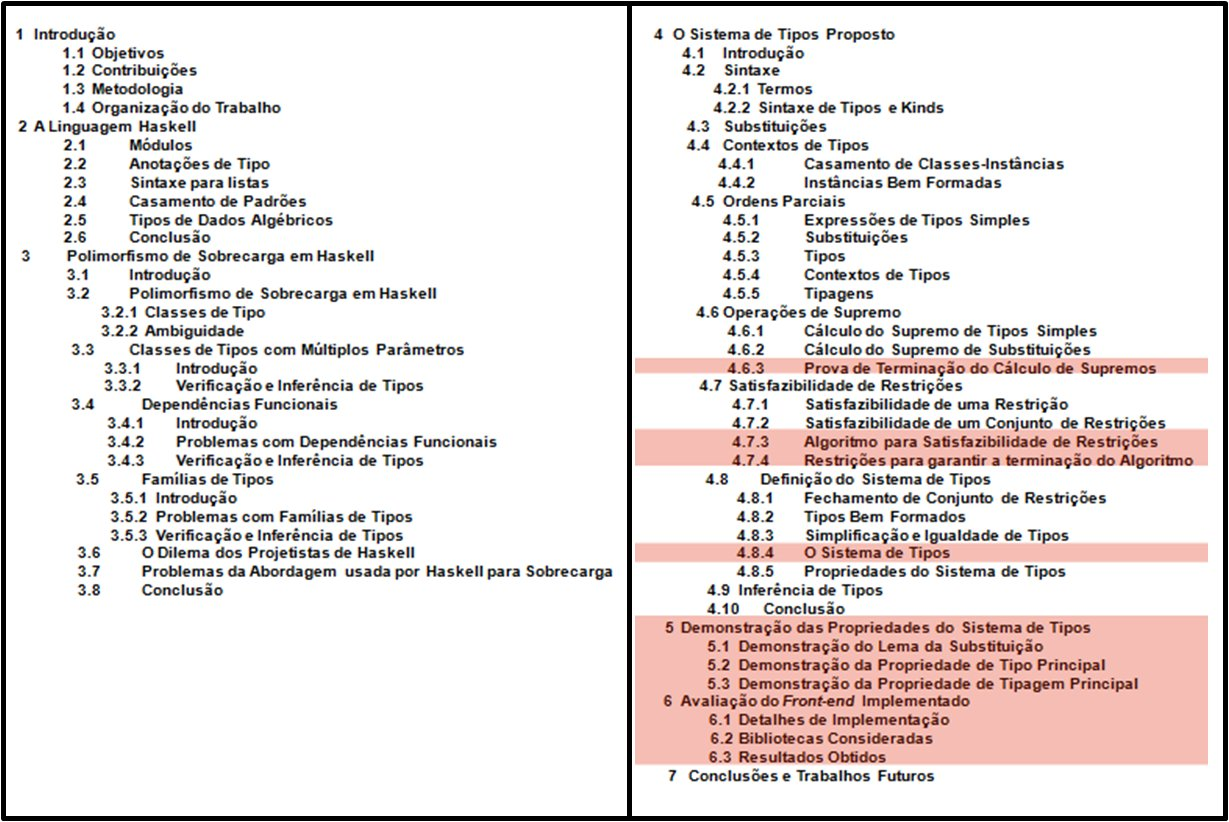
\includegraphics[scale=0.5]{sumario.jpg}
	\caption{Sum\'ario da Tese}
	\label{sumario}
\end{figure}		

O cronograma das atividades a serem realizadas \'e apresentado na figura \ref{cronograma}.

\begin{figure}[t]			
	\centering
	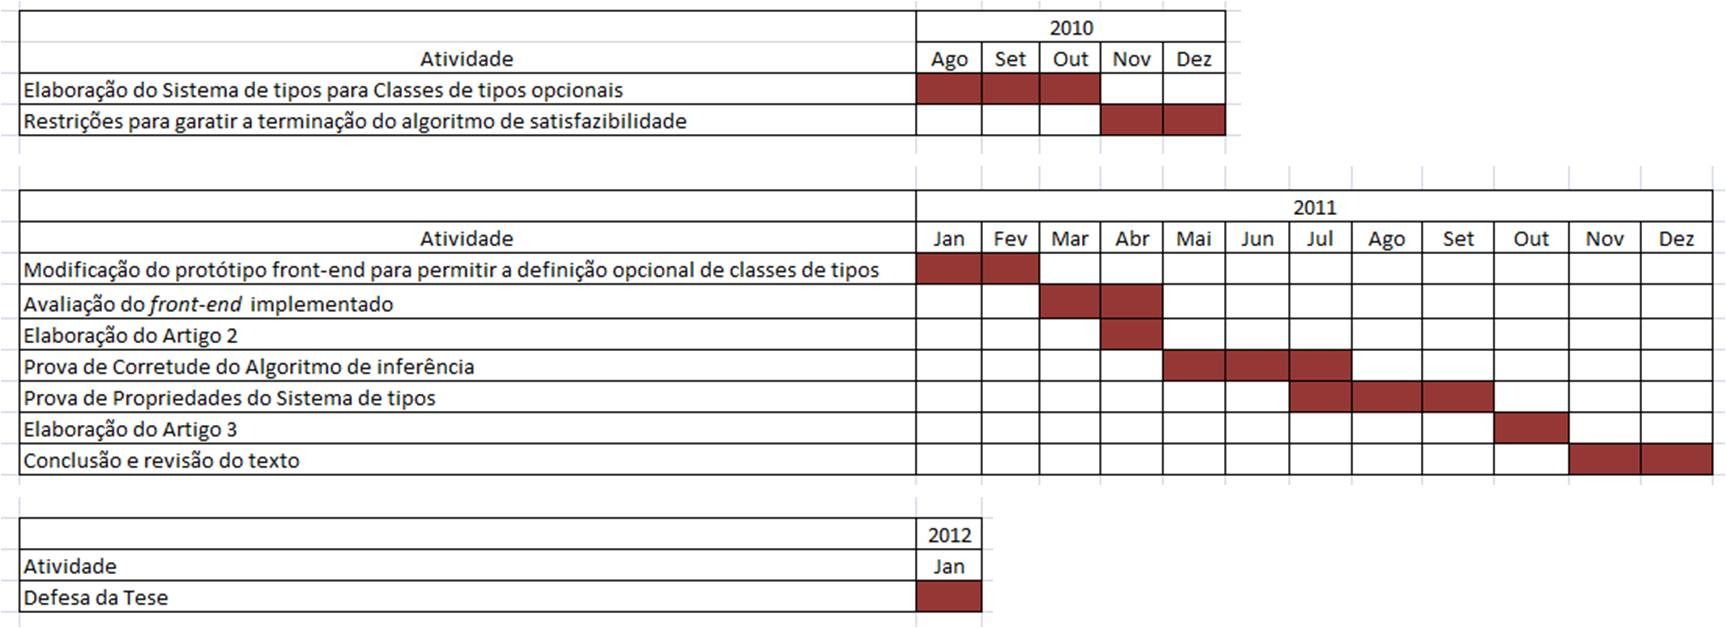
\includegraphics[scale=0.5]{cronograma.jpg}
	\caption{Cronograma das Atividades}
	\label{cronograma}
\end{figure}	

	\ppgccbibliography{document}
\end{document}
